\documentclass{book}
\usepackage[a4paper,top=2.5cm,bottom=2.5cm,left=2.5cm,right=2.5cm]{geometry}
\usepackage{makeidx}
\usepackage{natbib}
\usepackage{graphicx}
\usepackage{multicol}
\usepackage{float}
\usepackage{listings}
\usepackage{color}
\usepackage{ifthen}
\usepackage[table]{xcolor}
\usepackage{textcomp}
\usepackage{alltt}
\usepackage{ifpdf}
\ifpdf
\usepackage[pdftex,
            pagebackref=true,
            colorlinks=true,
            linkcolor=blue,
            unicode
           ]{hyperref}
\else
\usepackage[ps2pdf,
            pagebackref=true,
            colorlinks=true,
            linkcolor=blue,
            unicode
           ]{hyperref}
\usepackage{pspicture}
\fi
\usepackage[utf8]{inputenc}
\usepackage{mathptmx}
\usepackage[scaled=.90]{helvet}
\usepackage{courier}
\usepackage{sectsty}
\usepackage{amssymb}
\usepackage[titles]{tocloft}
\usepackage{doxygen}
\lstset{language=C++,inputencoding=utf8,basicstyle=\footnotesize,breaklines=true,breakatwhitespace=true,tabsize=8,numbers=left }
\makeindex
\setcounter{tocdepth}{3}
\renewcommand{\footrulewidth}{0.4pt}
\renewcommand{\familydefault}{\sfdefault}
\hfuzz=15pt
\setlength{\emergencystretch}{15pt}
\hbadness=750
\tolerance=750
\begin{document}
\hypersetup{pageanchor=false,citecolor=blue}
\begin{titlepage}
\vspace*{7cm}
\begin{center}
{\Large Hellfire\-O\-S v2.0 }\\
\vspace*{1cm}
{\large Generated by Doxygen 1.8.1.2}\\
\vspace*{0.5cm}
{\small Tue Aug 23 2016 19:41:09}\\
\end{center}
\end{titlepage}
\clearemptydoublepage
\pagenumbering{roman}
\tableofcontents
\clearemptydoublepage
\pagenumbering{arabic}
\hypersetup{pageanchor=true,citecolor=blue}
\chapter{Data Structure Index}
\section{Data Structures}
Here are the data structures with brief descriptions\-:\begin{DoxyCompactList}
\item\contentsline{section}{\hyperlink{structcondvar}{condvar} \\*Condition variable data structure }{\pageref{structcondvar}}{}
\item\contentsline{section}{\hyperlink{structlist}{list} \\*List data structure }{\pageref{structlist}}{}
\item\contentsline{section}{\hyperlink{structmailbox}{mailbox} \\*Mailbox data structure }{\pageref{structmailbox}}{}
\item\contentsline{section}{\hyperlink{structmem__block}{mem\-\_\-block} }{\pageref{structmem__block}}{}
\item\contentsline{section}{\hyperlink{structmem__chunk}{mem\-\_\-chunk} }{\pageref{structmem__chunk}}{}
\item\contentsline{section}{\hyperlink{structmem__chunk__ptr}{mem\-\_\-chunk\-\_\-ptr} }{\pageref{structmem__chunk__ptr}}{}
\item\contentsline{section}{\hyperlink{unionmem__header__union}{mem\-\_\-header\-\_\-union} }{\pageref{unionmem__header__union}}{}
\item\contentsline{section}{\hyperlink{structmtx}{mtx} \\*Mutex data structure }{\pageref{structmtx}}{}
\item\contentsline{section}{\hyperlink{structpcb__entry}{pcb\-\_\-entry} }{\pageref{structpcb__entry}}{}
\item\contentsline{section}{\hyperlink{structqueue}{queue} \\*Queue data structure }{\pageref{structqueue}}{}
\item\contentsline{section}{\hyperlink{structsem}{sem} \\*Semaphore data structure }{\pageref{structsem}}{}
\item\contentsline{section}{\hyperlink{structtcb__entry}{tcb\-\_\-entry} \\*Task control block (T\-C\-B) and processor control block (P\-C\-B) entry data structures }{\pageref{structtcb__entry}}{}
\end{DoxyCompactList}

\chapter{File Index}
\section{File List}
Here is a list of all files with brief descriptions\-:\begin{DoxyCompactList}
\item\contentsline{section}{drivers/noc/\hyperlink{noc_8c}{noc.\-c} }{\pageref{noc_8c}}{}
\item\contentsline{section}{drivers/noc/include/\hyperlink{noc_8h}{noc.\-h} }{\pageref{noc_8h}}{}
\item\contentsline{section}{sys/include/\hyperlink{condvar_8h}{condvar.\-h} }{\pageref{condvar_8h}}{}
\item\contentsline{section}{sys/include/\hyperlink{ecodes_8h}{ecodes.\-h} }{\pageref{ecodes_8h}}{}
\item\contentsline{section}{sys/include/\hyperlink{hellfire_8h}{hellfire.\-h} }{\pageref{hellfire_8h}}{}
\item\contentsline{section}{sys/include/\hyperlink{kernel_8h}{kernel.\-h} }{\pageref{kernel_8h}}{}
\item\contentsline{section}{sys/include/\hyperlink{kprintf_8h}{kprintf.\-h} }{\pageref{kprintf_8h}}{}
\item\contentsline{section}{sys/include/\hyperlink{list_8h}{list.\-h} }{\pageref{list_8h}}{}
\item\contentsline{section}{sys/include/\hyperlink{mailbox_8h}{mailbox.\-h} }{\pageref{mailbox_8h}}{}
\item\contentsline{section}{sys/include/\hyperlink{main_8h}{main.\-h} }{\pageref{main_8h}}{}
\item\contentsline{section}{sys/include/\hyperlink{malloc_8h}{malloc.\-h} }{\pageref{malloc_8h}}{}
\item\contentsline{section}{sys/include/\hyperlink{mutex_8h}{mutex.\-h} }{\pageref{mutex_8h}}{}
\item\contentsline{section}{sys/include/\hyperlink{panic_8h}{panic.\-h} }{\pageref{panic_8h}}{}
\item\contentsline{section}{sys/include/\hyperlink{processor_8h}{processor.\-h} }{\pageref{processor_8h}}{}
\item\contentsline{section}{sys/include/\hyperlink{queue_8h}{queue.\-h} }{\pageref{queue_8h}}{}
\item\contentsline{section}{sys/include/\hyperlink{scheduler_8h}{scheduler.\-h} }{\pageref{scheduler_8h}}{}
\item\contentsline{section}{sys/include/\hyperlink{semaphore_8h}{semaphore.\-h} }{\pageref{semaphore_8h}}{}
\item\contentsline{section}{sys/include/\hyperlink{task_8h}{task.\-h} }{\pageref{task_8h}}{}
\item\contentsline{section}{sys/kernel/\hyperlink{main_8c}{main.\-c} }{\pageref{main_8c}}{}
\item\contentsline{section}{sys/kernel/\hyperlink{panic_8c}{panic.\-c} }{\pageref{panic_8c}}{}
\item\contentsline{section}{sys/kernel/\hyperlink{processor_8c}{processor.\-c} }{\pageref{processor_8c}}{}
\item\contentsline{section}{sys/kernel/\hyperlink{scheduler_8c}{scheduler.\-c} }{\pageref{scheduler_8c}}{}
\item\contentsline{section}{sys/kernel/\hyperlink{task_8c}{task.\-c} }{\pageref{task_8c}}{}
\item\contentsline{section}{sys/lib/\hyperlink{kprintf_8c}{kprintf.\-c} }{\pageref{kprintf_8c}}{}
\item\contentsline{section}{sys/lib/\hyperlink{list_8c}{list.\-c} }{\pageref{list_8c}}{}
\item\contentsline{section}{sys/lib/\hyperlink{malloc_8c}{malloc.\-c} }{\pageref{malloc_8c}}{}
\item\contentsline{section}{sys/lib/\hyperlink{queue_8c}{queue.\-c} }{\pageref{queue_8c}}{}
\item\contentsline{section}{sys/sync/\hyperlink{condvar_8c}{condvar.\-c} }{\pageref{condvar_8c}}{}
\item\contentsline{section}{sys/sync/\hyperlink{mutex_8c}{mutex.\-c} }{\pageref{mutex_8c}}{}
\item\contentsline{section}{sys/sync/\hyperlink{semaphore_8c}{semaphore.\-c} }{\pageref{semaphore_8c}}{}
\end{DoxyCompactList}

\chapter{Data Structure Documentation}
\hypertarget{structcondvar}{\section{condvar Struct Reference}
\label{structcondvar}\index{condvar@{condvar}}
}


Condition variable data structure.  




{\ttfamily \#include $<$condvar.\-h$>$}



Collaboration diagram for condvar\-:\nopagebreak
\begin{figure}[H]
\begin{center}
\leavevmode
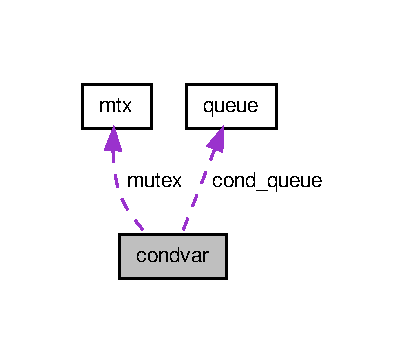
\includegraphics[width=195pt]{structcondvar__coll__graph}
\end{center}
\end{figure}
\subsection*{Data Fields}
\begin{DoxyCompactItemize}
\item 
struct \hyperlink{structqueue}{queue} $\ast$ \hyperlink{structcondvar_abf91dd97763d95af19ee92a17f55afb8}{cond\-\_\-queue}
\item 
\hyperlink{mutex_8h_a5d47ad3a25c2df1eecad005e0649a431}{mutex\-\_\-t} \hyperlink{structcondvar_a573f1b5d528d692d581b734913807b66}{mutex}
\end{DoxyCompactItemize}


\subsection{Detailed Description}
Condition variable data structure. 

\subsection{Field Documentation}
\hypertarget{structcondvar_abf91dd97763d95af19ee92a17f55afb8}{\index{condvar@{condvar}!cond\-\_\-queue@{cond\-\_\-queue}}
\index{cond\-\_\-queue@{cond\-\_\-queue}!condvar@{condvar}}
\subsubsection[{cond\-\_\-queue}]{\setlength{\rightskip}{0pt plus 5cm}struct {\bf queue}$\ast$ condvar\-::cond\-\_\-queue}}\label{structcondvar_abf91dd97763d95af19ee92a17f55afb8}
queue for tasks waiting on the condition variable \hypertarget{structcondvar_a573f1b5d528d692d581b734913807b66}{\index{condvar@{condvar}!mutex@{mutex}}
\index{mutex@{mutex}!condvar@{condvar}}
\subsubsection[{mutex}]{\setlength{\rightskip}{0pt plus 5cm}{\bf mutex\-\_\-t} condvar\-::mutex}}\label{structcondvar_a573f1b5d528d692d581b734913807b66}
mutex used for the critical section associated with the condition variable 

The documentation for this struct was generated from the following file\-:\begin{DoxyCompactItemize}
\item 
sys/include/\hyperlink{condvar_8h}{condvar.\-h}\end{DoxyCompactItemize}

\hypertarget{structlist}{\section{list Struct Reference}
\label{structlist}\index{list@{list}}
}


List data structure.  




{\ttfamily \#include $<$list.\-h$>$}



Collaboration diagram for list\-:\nopagebreak
\begin{figure}[H]
\begin{center}
\leavevmode
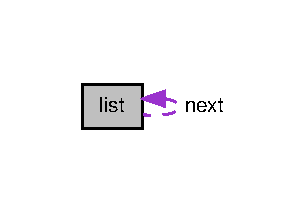
\includegraphics[width=148pt]{structlist__coll__graph}
\end{center}
\end{figure}
\subsection*{Data Fields}
\begin{DoxyCompactItemize}
\item 
void $\ast$ \hyperlink{structlist_af3f79a2886a3f27cdfdfa202c2affc68}{elem}
\item 
struct \hyperlink{structlist}{list} $\ast$ \hyperlink{structlist_a1900fe79e875e2838625b2eb60837f8f}{next}
\end{DoxyCompactItemize}


\subsection{Detailed Description}
List data structure. 

\subsection{Field Documentation}
\hypertarget{structlist_af3f79a2886a3f27cdfdfa202c2affc68}{\index{list@{list}!elem@{elem}}
\index{elem@{elem}!list@{list}}
\subsubsection[{elem}]{\setlength{\rightskip}{0pt plus 5cm}void$\ast$ list\-::elem}}\label{structlist_af3f79a2886a3f27cdfdfa202c2affc68}
pointer to list node data \hypertarget{structlist_a1900fe79e875e2838625b2eb60837f8f}{\index{list@{list}!next@{next}}
\index{next@{next}!list@{list}}
\subsubsection[{next}]{\setlength{\rightskip}{0pt plus 5cm}struct {\bf list}$\ast$ list\-::next}}\label{structlist_a1900fe79e875e2838625b2eb60837f8f}
pointer to the next list node 

The documentation for this struct was generated from the following file\-:\begin{DoxyCompactItemize}
\item 
sys/include/\hyperlink{list_8h}{list.\-h}\end{DoxyCompactItemize}

\hypertarget{structmailbox}{\section{mailbox Struct Reference}
\label{structmailbox}\index{mailbox@{mailbox}}
}


Mailbox data structure.  




{\ttfamily \#include $<$mailbox.\-h$>$}



Collaboration diagram for mailbox\-:\nopagebreak
\begin{figure}[H]
\begin{center}
\leavevmode
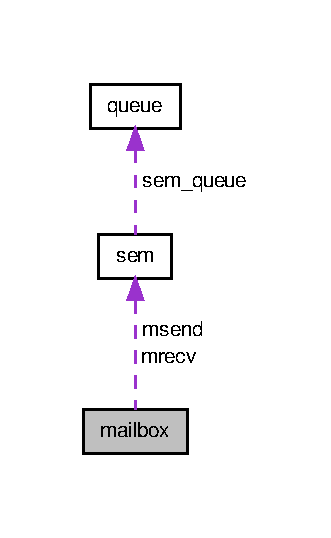
\includegraphics[width=159pt]{structmailbox__coll__graph}
\end{center}
\end{figure}
\subsection*{Data Fields}
\begin{DoxyCompactItemize}
\item 
void $\ast$ \hyperlink{structmailbox_a2568c0b3f722bca8beb8e85824806258}{msg}
\item 
uint16\-\_\-t \hyperlink{structmailbox_a7d31234908ebf91baf3dfbc8507f823e}{n\-\_\-waiting\-\_\-tasks}
\item 
uint16\-\_\-t \hyperlink{structmailbox_ae99432557a6663a6e7b43b27b4448c9c}{count}
\item 
\hyperlink{semaphore_8h_ad7630848c81d49708045a351922eb6b5}{sem\-\_\-t} \hyperlink{structmailbox_a061152c5d6eb8b70f1056c385c6cce73}{msend}
\item 
\hyperlink{semaphore_8h_ad7630848c81d49708045a351922eb6b5}{sem\-\_\-t} \hyperlink{structmailbox_aab51b97fffcc79e7398d8fadd8b0d3cb}{mrecv}
\end{DoxyCompactItemize}


\subsection{Detailed Description}
Mailbox data structure. 

\subsection{Field Documentation}
\hypertarget{structmailbox_ae99432557a6663a6e7b43b27b4448c9c}{\index{mailbox@{mailbox}!count@{count}}
\index{count@{count}!mailbox@{mailbox}}
\subsubsection[{count}]{\setlength{\rightskip}{0pt plus 5cm}uint16\-\_\-t mailbox\-::count}}\label{structmailbox_ae99432557a6663a6e7b43b27b4448c9c}
number of elements on the mailbox \hypertarget{structmailbox_aab51b97fffcc79e7398d8fadd8b0d3cb}{\index{mailbox@{mailbox}!mrecv@{mrecv}}
\index{mrecv@{mrecv}!mailbox@{mailbox}}
\subsubsection[{mrecv}]{\setlength{\rightskip}{0pt plus 5cm}{\bf sem\-\_\-t} mailbox\-::mrecv}}\label{structmailbox_aab51b97fffcc79e7398d8fadd8b0d3cb}
synchronization semaphore for mail receive \hypertarget{structmailbox_a061152c5d6eb8b70f1056c385c6cce73}{\index{mailbox@{mailbox}!msend@{msend}}
\index{msend@{msend}!mailbox@{mailbox}}
\subsubsection[{msend}]{\setlength{\rightskip}{0pt plus 5cm}{\bf sem\-\_\-t} mailbox\-::msend}}\label{structmailbox_a061152c5d6eb8b70f1056c385c6cce73}
synchronization semaphore for mail send \hypertarget{structmailbox_a2568c0b3f722bca8beb8e85824806258}{\index{mailbox@{mailbox}!msg@{msg}}
\index{msg@{msg}!mailbox@{mailbox}}
\subsubsection[{msg}]{\setlength{\rightskip}{0pt plus 5cm}void$\ast$ mailbox\-::msg}}\label{structmailbox_a2568c0b3f722bca8beb8e85824806258}
pointer to a message buffer \hypertarget{structmailbox_a7d31234908ebf91baf3dfbc8507f823e}{\index{mailbox@{mailbox}!n\-\_\-waiting\-\_\-tasks@{n\-\_\-waiting\-\_\-tasks}}
\index{n\-\_\-waiting\-\_\-tasks@{n\-\_\-waiting\-\_\-tasks}!mailbox@{mailbox}}
\subsubsection[{n\-\_\-waiting\-\_\-tasks}]{\setlength{\rightskip}{0pt plus 5cm}uint16\-\_\-t mailbox\-::n\-\_\-waiting\-\_\-tasks}}\label{structmailbox_a7d31234908ebf91baf3dfbc8507f823e}
number of waiting tasks in the mailbox 

The documentation for this struct was generated from the following file\-:\begin{DoxyCompactItemize}
\item 
sys/include/\hyperlink{mailbox_8h}{mailbox.\-h}\end{DoxyCompactItemize}

\hypertarget{structmem__block}{\section{mem\-\_\-block Struct Reference}
\label{structmem__block}\index{mem\-\_\-block@{mem\-\_\-block}}
}


{\ttfamily \#include $<$malloc.\-h$>$}



Collaboration diagram for mem\-\_\-block\-:\nopagebreak
\begin{figure}[H]
\begin{center}
\leavevmode
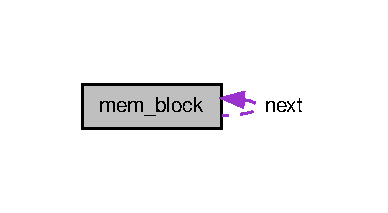
\includegraphics[width=186pt]{structmem__block__coll__graph}
\end{center}
\end{figure}
\subsection*{Data Fields}
\begin{DoxyCompactItemize}
\item 
struct \hyperlink{structmem__block}{mem\-\_\-block} $\ast$ \hyperlink{structmem__block_ac3317f1b6603856e265b1ba15c4a99b8}{next}
\item 
size\-\_\-t \hyperlink{structmem__block_a5ff4ee5dcd970bbc4951eb108c5eec4b}{size}
\end{DoxyCompactItemize}


\subsection{Field Documentation}
\hypertarget{structmem__block_ac3317f1b6603856e265b1ba15c4a99b8}{\index{mem\-\_\-block@{mem\-\_\-block}!next@{next}}
\index{next@{next}!mem_block@{mem\-\_\-block}}
\subsubsection[{next}]{\setlength{\rightskip}{0pt plus 5cm}struct {\bf mem\-\_\-block} $\ast$ mem\-\_\-block\-::next}}\label{structmem__block_ac3317f1b6603856e265b1ba15c4a99b8}
\hypertarget{structmem__block_a5ff4ee5dcd970bbc4951eb108c5eec4b}{\index{mem\-\_\-block@{mem\-\_\-block}!size@{size}}
\index{size@{size}!mem_block@{mem\-\_\-block}}
\subsubsection[{size}]{\setlength{\rightskip}{0pt plus 5cm}size\-\_\-t mem\-\_\-block\-::size}}\label{structmem__block_a5ff4ee5dcd970bbc4951eb108c5eec4b}


The documentation for this struct was generated from the following file\-:\begin{DoxyCompactItemize}
\item 
sys/include/\hyperlink{malloc_8h}{malloc.\-h}\end{DoxyCompactItemize}

\hypertarget{structmem__chunk}{\section{mem\-\_\-chunk Struct Reference}
\label{structmem__chunk}\index{mem\-\_\-chunk@{mem\-\_\-chunk}}
}


{\ttfamily \#include $<$malloc.\-h$>$}

\subsection*{Data Fields}
\begin{DoxyCompactItemize}
\item 
uint32\-\_\-t \hyperlink{structmem__chunk_a6c249814794488c18a42bcf180e3c024}{size}
\end{DoxyCompactItemize}


\subsection{Field Documentation}
\hypertarget{structmem__chunk_a6c249814794488c18a42bcf180e3c024}{\index{mem\-\_\-chunk@{mem\-\_\-chunk}!size@{size}}
\index{size@{size}!mem_chunk@{mem\-\_\-chunk}}
\subsubsection[{size}]{\setlength{\rightskip}{0pt plus 5cm}uint32\-\_\-t mem\-\_\-chunk\-::size}}\label{structmem__chunk_a6c249814794488c18a42bcf180e3c024}


The documentation for this struct was generated from the following file\-:\begin{DoxyCompactItemize}
\item 
sys/include/\hyperlink{malloc_8h}{malloc.\-h}\end{DoxyCompactItemize}

\hypertarget{structmem__chunk__ptr}{\section{mem\-\_\-chunk\-\_\-ptr Struct Reference}
\label{structmem__chunk__ptr}\index{mem\-\_\-chunk\-\_\-ptr@{mem\-\_\-chunk\-\_\-ptr}}
}


{\ttfamily \#include $<$malloc.\-h$>$}



Collaboration diagram for mem\-\_\-chunk\-\_\-ptr\-:\nopagebreak
\begin{figure}[H]
\begin{center}
\leavevmode
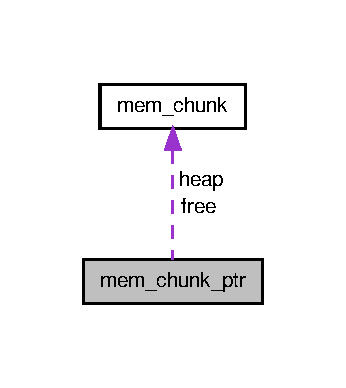
\includegraphics[width=166pt]{structmem__chunk__ptr__coll__graph}
\end{center}
\end{figure}
\subsection*{Data Fields}
\begin{DoxyCompactItemize}
\item 
\hyperlink{structmem__chunk}{mem\-\_\-chunk} $\ast$ \hyperlink{structmem__chunk__ptr_af7a1f60b420bd7ef98dde5a4cbc5bdf3}{free}
\item 
\hyperlink{structmem__chunk}{mem\-\_\-chunk} $\ast$ \hyperlink{structmem__chunk__ptr_aaddfb089e921369846e272d2d2b56e84}{heap}
\end{DoxyCompactItemize}


\subsection{Field Documentation}
\hypertarget{structmem__chunk__ptr_af7a1f60b420bd7ef98dde5a4cbc5bdf3}{\index{mem\-\_\-chunk\-\_\-ptr@{mem\-\_\-chunk\-\_\-ptr}!free@{free}}
\index{free@{free}!mem_chunk_ptr@{mem\-\_\-chunk\-\_\-ptr}}
\subsubsection[{free}]{\setlength{\rightskip}{0pt plus 5cm}{\bf mem\-\_\-chunk}$\ast$ mem\-\_\-chunk\-\_\-ptr\-::free}}\label{structmem__chunk__ptr_af7a1f60b420bd7ef98dde5a4cbc5bdf3}
\hypertarget{structmem__chunk__ptr_aaddfb089e921369846e272d2d2b56e84}{\index{mem\-\_\-chunk\-\_\-ptr@{mem\-\_\-chunk\-\_\-ptr}!heap@{heap}}
\index{heap@{heap}!mem_chunk_ptr@{mem\-\_\-chunk\-\_\-ptr}}
\subsubsection[{heap}]{\setlength{\rightskip}{0pt plus 5cm}{\bf mem\-\_\-chunk}$\ast$ mem\-\_\-chunk\-\_\-ptr\-::heap}}\label{structmem__chunk__ptr_aaddfb089e921369846e272d2d2b56e84}


The documentation for this struct was generated from the following file\-:\begin{DoxyCompactItemize}
\item 
sys/include/\hyperlink{malloc_8h}{malloc.\-h}\end{DoxyCompactItemize}

\hypertarget{unionmem__header__union}{\section{mem\-\_\-header\-\_\-union Union Reference}
\label{unionmem__header__union}\index{mem\-\_\-header\-\_\-union@{mem\-\_\-header\-\_\-union}}
}


{\ttfamily \#include $<$malloc.\-h$>$}



Collaboration diagram for mem\-\_\-header\-\_\-union\-:\nopagebreak
\begin{figure}[H]
\begin{center}
\leavevmode
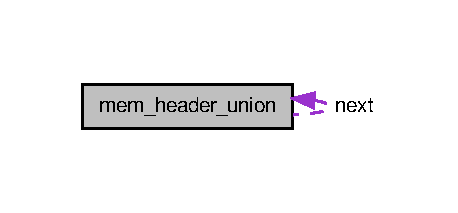
\includegraphics[width=220pt]{unionmem__header__union__coll__graph}
\end{center}
\end{figure}
\subsection*{Data Fields}
\begin{DoxyCompactItemize}
\item 
\begin{tabbing}
xx\=xx\=xx\=xx\=xx\=xx\=xx\=xx\=xx\=\kill
struct \{\\
\>union \hyperlink{unionmem__header__union}{mem\_header\_union} $\ast$ \hyperlink{unionmem__header__union_a22eb41be35488312c1e42462d5679d64}{next}\\
\>uint32\_t \hyperlink{unionmem__header__union_ab0a6578a8d52fd76a933d21273e73e08}{size}\\
\} \hyperlink{unionmem__header__union_a8e9bc77f2cf7596a7503f50ef29019f9}{s}\\

\end{tabbing}\item 
\hyperlink{malloc_8h_a1e0a98b5055eebe08414396335357f7f}{align} \hyperlink{unionmem__header__union_a5ca4f0da25cd2b76029162df7bdb537c}{align\-\_\-dummy}
\end{DoxyCompactItemize}


\subsection{Field Documentation}
\hypertarget{unionmem__header__union_a5ca4f0da25cd2b76029162df7bdb537c}{\index{mem\-\_\-header\-\_\-union@{mem\-\_\-header\-\_\-union}!align\-\_\-dummy@{align\-\_\-dummy}}
\index{align\-\_\-dummy@{align\-\_\-dummy}!mem_header_union@{mem\-\_\-header\-\_\-union}}
\subsubsection[{align\-\_\-dummy}]{\setlength{\rightskip}{0pt plus 5cm}{\bf align} mem\-\_\-header\-\_\-union\-::align\-\_\-dummy}}\label{unionmem__header__union_a5ca4f0da25cd2b76029162df7bdb537c}
\hypertarget{unionmem__header__union_a22eb41be35488312c1e42462d5679d64}{\index{mem\-\_\-header\-\_\-union@{mem\-\_\-header\-\_\-union}!next@{next}}
\index{next@{next}!mem_header_union@{mem\-\_\-header\-\_\-union}}
\subsubsection[{next}]{\setlength{\rightskip}{0pt plus 5cm}union {\bf mem\-\_\-header\-\_\-union}$\ast$ mem\-\_\-header\-\_\-union\-::next}}\label{unionmem__header__union_a22eb41be35488312c1e42462d5679d64}
\hypertarget{unionmem__header__union_a8e9bc77f2cf7596a7503f50ef29019f9}{\index{mem\-\_\-header\-\_\-union@{mem\-\_\-header\-\_\-union}!s@{s}}
\index{s@{s}!mem_header_union@{mem\-\_\-header\-\_\-union}}
\subsubsection[{s}]{\setlength{\rightskip}{0pt plus 5cm}struct \{ ... \}   mem\-\_\-header\-\_\-union\-::s}}\label{unionmem__header__union_a8e9bc77f2cf7596a7503f50ef29019f9}
\hypertarget{unionmem__header__union_ab0a6578a8d52fd76a933d21273e73e08}{\index{mem\-\_\-header\-\_\-union@{mem\-\_\-header\-\_\-union}!size@{size}}
\index{size@{size}!mem_header_union@{mem\-\_\-header\-\_\-union}}
\subsubsection[{size}]{\setlength{\rightskip}{0pt plus 5cm}uint32\-\_\-t mem\-\_\-header\-\_\-union\-::size}}\label{unionmem__header__union_ab0a6578a8d52fd76a933d21273e73e08}


The documentation for this union was generated from the following file\-:\begin{DoxyCompactItemize}
\item 
sys/include/\hyperlink{malloc_8h}{malloc.\-h}\end{DoxyCompactItemize}

\hypertarget{structmtx}{\section{mtx Struct Reference}
\label{structmtx}\index{mtx@{mtx}}
}


Mutex data structure.  




{\ttfamily \#include $<$mutex.\-h$>$}

\subsection*{Data Fields}
\begin{DoxyCompactItemize}
\item 
int32\-\_\-t \hyperlink{structmtx_a5c9abfe5d985f974f920b19b94890f40}{lock}
\item 
uint8\-\_\-t \hyperlink{structmtx_ab13e9d09a96e18160571b960e4e7c1fb}{level} \mbox{[}M\-A\-X\-\_\-\-T\-A\-S\-K\-S\mbox{]}
\item 
uint8\-\_\-t \hyperlink{structmtx_ab86ca9283ce5f816d3700d0212662e04}{waiting} \mbox{[}M\-A\-X\-\_\-\-T\-A\-S\-K\-S-\/1\mbox{]}
\end{DoxyCompactItemize}


\subsection{Detailed Description}
Mutex data structure. 

\subsection{Field Documentation}
\hypertarget{structmtx_ab13e9d09a96e18160571b960e4e7c1fb}{\index{mtx@{mtx}!level@{level}}
\index{level@{level}!mtx@{mtx}}
\subsubsection[{level}]{\setlength{\rightskip}{0pt plus 5cm}uint8\-\_\-t mtx\-::level\mbox{[}M\-A\-X\-\_\-\-T\-A\-S\-K\-S\mbox{]}}}\label{structmtx_ab13e9d09a96e18160571b960e4e7c1fb}
\hypertarget{structmtx_a5c9abfe5d985f974f920b19b94890f40}{\index{mtx@{mtx}!lock@{lock}}
\index{lock@{lock}!mtx@{mtx}}
\subsubsection[{lock}]{\setlength{\rightskip}{0pt plus 5cm}int32\-\_\-t mtx\-::lock}}\label{structmtx_a5c9abfe5d985f974f920b19b94890f40}
mutex lock, atomically modified \hypertarget{structmtx_ab86ca9283ce5f816d3700d0212662e04}{\index{mtx@{mtx}!waiting@{waiting}}
\index{waiting@{waiting}!mtx@{mtx}}
\subsubsection[{waiting}]{\setlength{\rightskip}{0pt plus 5cm}uint8\-\_\-t mtx\-::waiting\mbox{[}M\-A\-X\-\_\-\-T\-A\-S\-K\-S-\/1\mbox{]}}}\label{structmtx_ab86ca9283ce5f816d3700d0212662e04}


The documentation for this struct was generated from the following file\-:\begin{DoxyCompactItemize}
\item 
sys/include/\hyperlink{mutex_8h}{mutex.\-h}\end{DoxyCompactItemize}

\hypertarget{structpcb__entry}{\section{pcb\-\_\-entry Struct Reference}
\label{structpcb__entry}\index{pcb\-\_\-entry@{pcb\-\_\-entry}}
}


{\ttfamily \#include $<$kernel.\-h$>$}

\subsection*{Data Fields}
\begin{DoxyCompactItemize}
\item 
uint32\-\_\-t \hyperlink{structpcb__entry_ac5899befd89fa0e8b2aeceed85e01415}{coop\-\_\-cswitch}
\item 
uint32\-\_\-t \hyperlink{structpcb__entry_af49c7195c79f5de2d70825e2252c8d77}{preempt\-\_\-cswitch}
\item 
uint32\-\_\-t \hyperlink{structpcb__entry_ae5474e1d477335caf5515d8a940d1f77}{interrupts}
\end{DoxyCompactItemize}


\subsection{Field Documentation}
\hypertarget{structpcb__entry_ac5899befd89fa0e8b2aeceed85e01415}{\index{pcb\-\_\-entry@{pcb\-\_\-entry}!coop\-\_\-cswitch@{coop\-\_\-cswitch}}
\index{coop\-\_\-cswitch@{coop\-\_\-cswitch}!pcb_entry@{pcb\-\_\-entry}}
\subsubsection[{coop\-\_\-cswitch}]{\setlength{\rightskip}{0pt plus 5cm}uint32\-\_\-t pcb\-\_\-entry\-::coop\-\_\-cswitch}}\label{structpcb__entry_ac5899befd89fa0e8b2aeceed85e01415}
cooperative context switches \hypertarget{structpcb__entry_ae5474e1d477335caf5515d8a940d1f77}{\index{pcb\-\_\-entry@{pcb\-\_\-entry}!interrupts@{interrupts}}
\index{interrupts@{interrupts}!pcb_entry@{pcb\-\_\-entry}}
\subsubsection[{interrupts}]{\setlength{\rightskip}{0pt plus 5cm}uint32\-\_\-t pcb\-\_\-entry\-::interrupts}}\label{structpcb__entry_ae5474e1d477335caf5515d8a940d1f77}
number of non-\/masked interrupts \hypertarget{structpcb__entry_af49c7195c79f5de2d70825e2252c8d77}{\index{pcb\-\_\-entry@{pcb\-\_\-entry}!preempt\-\_\-cswitch@{preempt\-\_\-cswitch}}
\index{preempt\-\_\-cswitch@{preempt\-\_\-cswitch}!pcb_entry@{pcb\-\_\-entry}}
\subsubsection[{preempt\-\_\-cswitch}]{\setlength{\rightskip}{0pt plus 5cm}uint32\-\_\-t pcb\-\_\-entry\-::preempt\-\_\-cswitch}}\label{structpcb__entry_af49c7195c79f5de2d70825e2252c8d77}
preeptive context switches 

The documentation for this struct was generated from the following file\-:\begin{DoxyCompactItemize}
\item 
sys/include/\hyperlink{kernel_8h}{kernel.\-h}\end{DoxyCompactItemize}

\hypertarget{structqueue}{\section{queue Struct Reference}
\label{structqueue}\index{queue@{queue}}
}


Queue data structure.  




{\ttfamily \#include $<$queue.\-h$>$}

\subsection*{Data Fields}
\begin{DoxyCompactItemize}
\item 
int32\-\_\-t \hyperlink{structqueue_af80cfabc36286195365b6d666d518504}{size}
\item 
int32\-\_\-t \hyperlink{structqueue_a187a42d061b48da53e894181758d558d}{elem}
\item 
int32\-\_\-t \hyperlink{structqueue_aec96f7889213946d685f28a0d6504428}{head}
\item 
int32\-\_\-t \hyperlink{structqueue_ada0fe9a078df1d07623c761f2e8376ad}{tail}
\item 
void $\ast$$\ast$ \hyperlink{structqueue_a794929032d575599c02f795cea4b3118}{data}
\end{DoxyCompactItemize}


\subsection{Detailed Description}
Queue data structure. 

\subsection{Field Documentation}
\hypertarget{structqueue_a794929032d575599c02f795cea4b3118}{\index{queue@{queue}!data@{data}}
\index{data@{data}!queue@{queue}}
\subsubsection[{data}]{\setlength{\rightskip}{0pt plus 5cm}void$\ast$$\ast$ queue\-::data}}\label{structqueue_a794929032d575599c02f795cea4b3118}
pointer to an array of pointers to node data \hypertarget{structqueue_a187a42d061b48da53e894181758d558d}{\index{queue@{queue}!elem@{elem}}
\index{elem@{elem}!queue@{queue}}
\subsubsection[{elem}]{\setlength{\rightskip}{0pt plus 5cm}int32\-\_\-t queue\-::elem}}\label{structqueue_a187a42d061b48da53e894181758d558d}
number of elements queued \hypertarget{structqueue_aec96f7889213946d685f28a0d6504428}{\index{queue@{queue}!head@{head}}
\index{head@{head}!queue@{queue}}
\subsubsection[{head}]{\setlength{\rightskip}{0pt plus 5cm}int32\-\_\-t queue\-::head}}\label{structqueue_aec96f7889213946d685f28a0d6504428}
first element of the queue \hypertarget{structqueue_af80cfabc36286195365b6d666d518504}{\index{queue@{queue}!size@{size}}
\index{size@{size}!queue@{queue}}
\subsubsection[{size}]{\setlength{\rightskip}{0pt plus 5cm}int32\-\_\-t queue\-::size}}\label{structqueue_af80cfabc36286195365b6d666d518504}
queue size (maximum number of elements) \hypertarget{structqueue_ada0fe9a078df1d07623c761f2e8376ad}{\index{queue@{queue}!tail@{tail}}
\index{tail@{tail}!queue@{queue}}
\subsubsection[{tail}]{\setlength{\rightskip}{0pt plus 5cm}int32\-\_\-t queue\-::tail}}\label{structqueue_ada0fe9a078df1d07623c761f2e8376ad}
last element of the queue 

The documentation for this struct was generated from the following file\-:\begin{DoxyCompactItemize}
\item 
sys/include/\hyperlink{queue_8h}{queue.\-h}\end{DoxyCompactItemize}

\hypertarget{structsem}{\section{sem Struct Reference}
\label{structsem}\index{sem@{sem}}
}


Semaphore data structure.  




{\ttfamily \#include $<$semaphore.\-h$>$}



Collaboration diagram for sem\-:\nopagebreak
\begin{figure}[H]
\begin{center}
\leavevmode
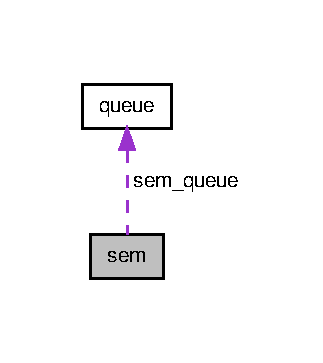
\includegraphics[width=155pt]{structsem__coll__graph}
\end{center}
\end{figure}
\subsection*{Data Fields}
\begin{DoxyCompactItemize}
\item 
struct \hyperlink{structqueue}{queue} $\ast$ \hyperlink{structsem_a723ac960b2566b855b905fa4aa324f9b}{sem\-\_\-queue}
\item 
int32\-\_\-t \hyperlink{structsem_a798dc7e825b1e632b2db49b473b17636}{count}
\end{DoxyCompactItemize}


\subsection{Detailed Description}
Semaphore data structure. 

\subsection{Field Documentation}
\hypertarget{structsem_a798dc7e825b1e632b2db49b473b17636}{\index{sem@{sem}!count@{count}}
\index{count@{count}!sem@{sem}}
\subsubsection[{count}]{\setlength{\rightskip}{0pt plus 5cm}int32\-\_\-t sem\-::count}}\label{structsem_a798dc7e825b1e632b2db49b473b17636}
semaphore counter \hypertarget{structsem_a723ac960b2566b855b905fa4aa324f9b}{\index{sem@{sem}!sem\-\_\-queue@{sem\-\_\-queue}}
\index{sem\-\_\-queue@{sem\-\_\-queue}!sem@{sem}}
\subsubsection[{sem\-\_\-queue}]{\setlength{\rightskip}{0pt plus 5cm}struct {\bf queue}$\ast$ sem\-::sem\-\_\-queue}}\label{structsem_a723ac960b2566b855b905fa4aa324f9b}
queue for tasks waiting on the semaphore 

The documentation for this struct was generated from the following file\-:\begin{DoxyCompactItemize}
\item 
sys/include/\hyperlink{semaphore_8h}{semaphore.\-h}\end{DoxyCompactItemize}

\hypertarget{structtcb__entry}{\section{tcb\-\_\-entry Struct Reference}
\label{structtcb__entry}\index{tcb\-\_\-entry@{tcb\-\_\-entry}}
}


Task control block (T\-C\-B) and processor control block (P\-C\-B) entry data structures.  




{\ttfamily \#include $<$kernel.\-h$>$}

\subsection*{Data Fields}
\begin{DoxyCompactItemize}
\item 
uint16\-\_\-t \hyperlink{structtcb__entry_ac06c8d6513b9d3031956b0efc2ab4871}{id}
\item 
int8\-\_\-t \hyperlink{structtcb__entry_ad7bfcb0f4b58b797af44f3a078abebff}{name} \mbox{[}20\mbox{]}
\item 
uint8\-\_\-t \hyperlink{structtcb__entry_a67f430ab50cb8ff9133e133fc240f3d7}{state}
\item 
uint32\-\_\-t \hyperlink{structtcb__entry_ab29fad6168f140493ddc8f860fadc3bc}{delay}
\item 
uint32\-\_\-t \hyperlink{structtcb__entry_a51802bc7ba3ee4cfcbcbfb404e606643}{rtjobs}
\item 
uint32\-\_\-t \hyperlink{structtcb__entry_a27631962295edabd283477b471f2d7ae}{bgjobs}
\item 
uint32\-\_\-t \hyperlink{structtcb__entry_a4594d17577feba0bd0825c8ef5e693db}{deadline\-\_\-misses}
\item 
uint16\-\_\-t \hyperlink{structtcb__entry_a85e14b4c040e0535b45b52a7ee7c9a94}{period}
\item 
uint16\-\_\-t \hyperlink{structtcb__entry_a2a3c8e5e81c910ccd845a8d1f58d550a}{capacity}
\item 
uint16\-\_\-t \hyperlink{structtcb__entry_a14ef4f38d7589e42ac7847b2bcc3443f}{deadline}
\item 
uint16\-\_\-t \hyperlink{structtcb__entry_a559dce8ac2982d3c8f46808ddc52bbb9}{capacity\-\_\-rem}
\item 
uint16\-\_\-t \hyperlink{structtcb__entry_af2ba0dde6c7ae71b6341714bf096cc80}{deadline\-\_\-rem}
\item 
context \hyperlink{structtcb__entry_a589e6c94b17a97df5d22edf504acfd42}{task\-\_\-context}
\item 
void($\ast$ \hyperlink{structtcb__entry_a7ed7f2d228da0039f065f0c8a756b46d}{ptask} )(void)
\item 
int32\-\_\-t $\ast$ \hyperlink{structtcb__entry_a0434be5f20d1645ab2804b7ee5c95fc9}{pstack}
\item 
uint32\-\_\-t \hyperlink{structtcb__entry_a2174ff4c5cf178e9dc3d652c472b23dd}{stack\-\_\-size}
\item 
void $\ast$ \hyperlink{structtcb__entry_accd675f017bb0ec5ae63b4d729bd73aa}{other\-\_\-data}
\end{DoxyCompactItemize}


\subsection{Detailed Description}
Task control block (T\-C\-B) and processor control block (P\-C\-B) entry data structures. 

\subsection{Field Documentation}
\hypertarget{structtcb__entry_a27631962295edabd283477b471f2d7ae}{\index{tcb\-\_\-entry@{tcb\-\_\-entry}!bgjobs@{bgjobs}}
\index{bgjobs@{bgjobs}!tcb_entry@{tcb\-\_\-entry}}
\subsubsection[{bgjobs}]{\setlength{\rightskip}{0pt plus 5cm}uint32\-\_\-t tcb\-\_\-entry\-::bgjobs}}\label{structtcb__entry_a27631962295edabd283477b471f2d7ae}
total B\-E jobs executed. B\-E tasks share processor idle time and execute in the background. \hypertarget{structtcb__entry_a2a3c8e5e81c910ccd845a8d1f58d550a}{\index{tcb\-\_\-entry@{tcb\-\_\-entry}!capacity@{capacity}}
\index{capacity@{capacity}!tcb_entry@{tcb\-\_\-entry}}
\subsubsection[{capacity}]{\setlength{\rightskip}{0pt plus 5cm}uint16\-\_\-t tcb\-\_\-entry\-::capacity}}\label{structtcb__entry_a2a3c8e5e81c910ccd845a8d1f58d550a}
task capacity \hypertarget{structtcb__entry_a559dce8ac2982d3c8f46808ddc52bbb9}{\index{tcb\-\_\-entry@{tcb\-\_\-entry}!capacity\-\_\-rem@{capacity\-\_\-rem}}
\index{capacity\-\_\-rem@{capacity\-\_\-rem}!tcb_entry@{tcb\-\_\-entry}}
\subsubsection[{capacity\-\_\-rem}]{\setlength{\rightskip}{0pt plus 5cm}uint16\-\_\-t tcb\-\_\-entry\-::capacity\-\_\-rem}}\label{structtcb__entry_a559dce8ac2982d3c8f46808ddc52bbb9}
remaining capacity on period \hypertarget{structtcb__entry_a14ef4f38d7589e42ac7847b2bcc3443f}{\index{tcb\-\_\-entry@{tcb\-\_\-entry}!deadline@{deadline}}
\index{deadline@{deadline}!tcb_entry@{tcb\-\_\-entry}}
\subsubsection[{deadline}]{\setlength{\rightskip}{0pt plus 5cm}uint16\-\_\-t tcb\-\_\-entry\-::deadline}}\label{structtcb__entry_a14ef4f38d7589e42ac7847b2bcc3443f}
task deadline \hypertarget{structtcb__entry_a4594d17577feba0bd0825c8ef5e693db}{\index{tcb\-\_\-entry@{tcb\-\_\-entry}!deadline\-\_\-misses@{deadline\-\_\-misses}}
\index{deadline\-\_\-misses@{deadline\-\_\-misses}!tcb_entry@{tcb\-\_\-entry}}
\subsubsection[{deadline\-\_\-misses}]{\setlength{\rightskip}{0pt plus 5cm}uint32\-\_\-t tcb\-\_\-entry\-::deadline\-\_\-misses}}\label{structtcb__entry_a4594d17577feba0bd0825c8ef5e693db}
task realtime deadline misses \hypertarget{structtcb__entry_af2ba0dde6c7ae71b6341714bf096cc80}{\index{tcb\-\_\-entry@{tcb\-\_\-entry}!deadline\-\_\-rem@{deadline\-\_\-rem}}
\index{deadline\-\_\-rem@{deadline\-\_\-rem}!tcb_entry@{tcb\-\_\-entry}}
\subsubsection[{deadline\-\_\-rem}]{\setlength{\rightskip}{0pt plus 5cm}uint16\-\_\-t tcb\-\_\-entry\-::deadline\-\_\-rem}}\label{structtcb__entry_af2ba0dde6c7ae71b6341714bf096cc80}
remaining time slices on period \hypertarget{structtcb__entry_ab29fad6168f140493ddc8f860fadc3bc}{\index{tcb\-\_\-entry@{tcb\-\_\-entry}!delay@{delay}}
\index{delay@{delay}!tcb_entry@{tcb\-\_\-entry}}
\subsubsection[{delay}]{\setlength{\rightskip}{0pt plus 5cm}uint32\-\_\-t tcb\-\_\-entry\-::delay}}\label{structtcb__entry_ab29fad6168f140493ddc8f860fadc3bc}
delay to enter in the run/\-R\-T queue \hypertarget{structtcb__entry_ac06c8d6513b9d3031956b0efc2ab4871}{\index{tcb\-\_\-entry@{tcb\-\_\-entry}!id@{id}}
\index{id@{id}!tcb_entry@{tcb\-\_\-entry}}
\subsubsection[{id}]{\setlength{\rightskip}{0pt plus 5cm}uint16\-\_\-t tcb\-\_\-entry\-::id}}\label{structtcb__entry_ac06c8d6513b9d3031956b0efc2ab4871}
task id \hypertarget{structtcb__entry_ad7bfcb0f4b58b797af44f3a078abebff}{\index{tcb\-\_\-entry@{tcb\-\_\-entry}!name@{name}}
\index{name@{name}!tcb_entry@{tcb\-\_\-entry}}
\subsubsection[{name}]{\setlength{\rightskip}{0pt plus 5cm}int8\-\_\-t tcb\-\_\-entry\-::name\mbox{[}20\mbox{]}}}\label{structtcb__entry_ad7bfcb0f4b58b797af44f3a078abebff}
task description (or name) \hypertarget{structtcb__entry_accd675f017bb0ec5ae63b4d729bd73aa}{\index{tcb\-\_\-entry@{tcb\-\_\-entry}!other\-\_\-data@{other\-\_\-data}}
\index{other\-\_\-data@{other\-\_\-data}!tcb_entry@{tcb\-\_\-entry}}
\subsubsection[{other\-\_\-data}]{\setlength{\rightskip}{0pt plus 5cm}void$\ast$ tcb\-\_\-entry\-::other\-\_\-data}}\label{structtcb__entry_accd675f017bb0ec5ae63b4d729bd73aa}
pointer to other data related to this task \hypertarget{structtcb__entry_a85e14b4c040e0535b45b52a7ee7c9a94}{\index{tcb\-\_\-entry@{tcb\-\_\-entry}!period@{period}}
\index{period@{period}!tcb_entry@{tcb\-\_\-entry}}
\subsubsection[{period}]{\setlength{\rightskip}{0pt plus 5cm}uint16\-\_\-t tcb\-\_\-entry\-::period}}\label{structtcb__entry_a85e14b4c040e0535b45b52a7ee7c9a94}
task period \hypertarget{structtcb__entry_a0434be5f20d1645ab2804b7ee5c95fc9}{\index{tcb\-\_\-entry@{tcb\-\_\-entry}!pstack@{pstack}}
\index{pstack@{pstack}!tcb_entry@{tcb\-\_\-entry}}
\subsubsection[{pstack}]{\setlength{\rightskip}{0pt plus 5cm}int32\-\_\-t$\ast$ tcb\-\_\-entry\-::pstack}}\label{structtcb__entry_a0434be5f20d1645ab2804b7ee5c95fc9}
task stack area (bottom) \hypertarget{structtcb__entry_a7ed7f2d228da0039f065f0c8a756b46d}{\index{tcb\-\_\-entry@{tcb\-\_\-entry}!ptask@{ptask}}
\index{ptask@{ptask}!tcb_entry@{tcb\-\_\-entry}}
\subsubsection[{ptask}]{\setlength{\rightskip}{0pt plus 5cm}void($\ast$ tcb\-\_\-entry\-::ptask)(void)}}\label{structtcb__entry_a7ed7f2d228da0039f065f0c8a756b46d}
task entry point, pointer to function \hypertarget{structtcb__entry_a51802bc7ba3ee4cfcbcbfb404e606643}{\index{tcb\-\_\-entry@{tcb\-\_\-entry}!rtjobs@{rtjobs}}
\index{rtjobs@{rtjobs}!tcb_entry@{tcb\-\_\-entry}}
\subsubsection[{rtjobs}]{\setlength{\rightskip}{0pt plus 5cm}uint32\-\_\-t tcb\-\_\-entry\-::rtjobs}}\label{structtcb__entry_a51802bc7ba3ee4cfcbcbfb404e606643}
total R\-T task jobs executed \hypertarget{structtcb__entry_a2174ff4c5cf178e9dc3d652c472b23dd}{\index{tcb\-\_\-entry@{tcb\-\_\-entry}!stack\-\_\-size@{stack\-\_\-size}}
\index{stack\-\_\-size@{stack\-\_\-size}!tcb_entry@{tcb\-\_\-entry}}
\subsubsection[{stack\-\_\-size}]{\setlength{\rightskip}{0pt plus 5cm}uint32\-\_\-t tcb\-\_\-entry\-::stack\-\_\-size}}\label{structtcb__entry_a2174ff4c5cf178e9dc3d652c472b23dd}
task stack size \hypertarget{structtcb__entry_a67f430ab50cb8ff9133e133fc240f3d7}{\index{tcb\-\_\-entry@{tcb\-\_\-entry}!state@{state}}
\index{state@{state}!tcb_entry@{tcb\-\_\-entry}}
\subsubsection[{state}]{\setlength{\rightskip}{0pt plus 5cm}uint8\-\_\-t tcb\-\_\-entry\-::state}}\label{structtcb__entry_a67f430ab50cb8ff9133e133fc240f3d7}
0 -\/ idle, 1 -\/ ready, 2 -\/ running, 3 -\/ blocked, 4 -\/ delayed, 5 -\/ waiting \hypertarget{structtcb__entry_a589e6c94b17a97df5d22edf504acfd42}{\index{tcb\-\_\-entry@{tcb\-\_\-entry}!task\-\_\-context@{task\-\_\-context}}
\index{task\-\_\-context@{task\-\_\-context}!tcb_entry@{tcb\-\_\-entry}}
\subsubsection[{task\-\_\-context}]{\setlength{\rightskip}{0pt plus 5cm}context tcb\-\_\-entry\-::task\-\_\-context}}\label{structtcb__entry_a589e6c94b17a97df5d22edf504acfd42}
task context 

The documentation for this struct was generated from the following file\-:\begin{DoxyCompactItemize}
\item 
sys/include/\hyperlink{kernel_8h}{kernel.\-h}\end{DoxyCompactItemize}

\chapter{File Documentation}
\hypertarget{noc_8h}{\section{drivers/noc/include/noc.h File Reference}
\label{noc_8h}\index{drivers/noc/include/noc.\-h@{drivers/noc/include/noc.\-h}}
}
\subsection*{Functions}
\begin{DoxyCompactItemize}
\item 
void \hyperlink{noc_8h_acb44cf0de3a986b823c53d881bff9568}{ni\-\_\-init} (void)
\begin{DoxyCompactList}\small\item\em No\-C driver\-: initializes the network interface. \end{DoxyCompactList}\item 
void \hyperlink{noc_8h_a7ca8f6357767be7d8d8f31a1f68902a1}{ni\-\_\-isr} (void $\ast$arg)
\begin{DoxyCompactList}\small\item\em No\-C driver\-: network interface interrupt service routine. \end{DoxyCompactList}\item 
uint16\-\_\-t \hyperlink{noc_8h_a73af25121fa7d699224d30913bb3cfa9}{hf\-\_\-cpuid} (void)
\begin{DoxyCompactList}\small\item\em Returns the current cpu id number. \end{DoxyCompactList}\item 
uint16\-\_\-t \hyperlink{noc_8h_ac100d0cfa54da4cf1c8ffda0947a7509}{hf\-\_\-ncores} (void)
\begin{DoxyCompactList}\small\item\em Returns the number of processors in the system. \end{DoxyCompactList}\item 
int32\-\_\-t \hyperlink{noc_8h_a7cc950118783aff78ef381c30f411f31}{hf\-\_\-comm\-\_\-create} (uint16\-\_\-t id, uint16\-\_\-t port, uint16\-\_\-t packets)
\begin{DoxyCompactList}\small\item\em Creates a communication queue for a task, using a port number as an alias. \end{DoxyCompactList}\item 
int32\-\_\-t \hyperlink{noc_8h_a2ca5bce1d7d281b5ca1ee007b170143b}{hf\-\_\-comm\-\_\-destroy} (uint16\-\_\-t id)
\begin{DoxyCompactList}\small\item\em Destroys a communication queue, returning packets buffered on a task message queue to the shared pool of packets. \end{DoxyCompactList}\item 
int32\-\_\-t \hyperlink{noc_8h_a27bdcde2185022f68eece2e0ed1c20ec}{hf\-\_\-recv} (uint16\-\_\-t $\ast$source\-\_\-cpu, uint16\-\_\-t $\ast$source\-\_\-port, int8\-\_\-t $\ast$buf, uint16\-\_\-t $\ast$size, uint16\-\_\-t channel)
\begin{DoxyCompactList}\small\item\em Receives a message from a task (blocking receive). \end{DoxyCompactList}\item 
int32\-\_\-t \hyperlink{noc_8h_ae7c110f06bc1e123f03b2d52d8b6d70f}{hf\-\_\-send} (uint16\-\_\-t target\-\_\-cpu, uint16\-\_\-t target\-\_\-port, int8\-\_\-t $\ast$buf, uint16\-\_\-t size, uint16\-\_\-t channel)
\begin{DoxyCompactList}\small\item\em Sends a message to a task (blocking send). \end{DoxyCompactList}\item 
int32\-\_\-t \hyperlink{noc_8h_a264ff860d8ad312fea8d658b6c254f17}{hf\-\_\-recvack} (uint16\-\_\-t $\ast$source\-\_\-cpu, uint16\-\_\-t $\ast$source\-\_\-port, int8\-\_\-t $\ast$buf, uint16\-\_\-t $\ast$size, uint16\-\_\-t channel)
\begin{DoxyCompactList}\small\item\em Receives a message from a task (blocking receive) with acknowledgement. \end{DoxyCompactList}\item 
int32\-\_\-t \hyperlink{noc_8h_a288522d034824d53cf10c6f71bca41ea}{hf\-\_\-sendack} (uint16\-\_\-t target\-\_\-cpu, uint16\-\_\-t target\-\_\-port, int8\-\_\-t $\ast$buf, uint16\-\_\-t size, uint16\-\_\-t channel, uint32\-\_\-t timeout)
\begin{DoxyCompactList}\small\item\em Sends a message to a task (blocking send) with acknowledgement. \end{DoxyCompactList}\end{DoxyCompactItemize}
\subsection*{Variables}
\begin{DoxyCompactItemize}
\item 
uint16\-\_\-t \hyperlink{noc_8h_a28c51954b0e202d17770b6f597d58e35}{pktdrv\-\_\-ports} \mbox{[}M\-A\-X\-\_\-\-T\-A\-S\-K\-S\mbox{]}
\begin{DoxyCompactList}\small\item\em Array of associations between tasks and reception ports. \end{DoxyCompactList}\item 
struct \hyperlink{structqueue}{queue} $\ast$ \hyperlink{noc_8h_a6e2b90dbd05cdac119b8d3296579de0a}{pktdrv\-\_\-tqueue} \mbox{[}M\-A\-X\-\_\-\-T\-A\-S\-K\-S\mbox{]}
\begin{DoxyCompactList}\small\item\em Array of queues. Each task can have its own custom sized queue. \end{DoxyCompactList}\item 
struct \hyperlink{structqueue}{queue} $\ast$ \hyperlink{noc_8h_ac96abbb61b929a8293778fe63006aca4}{pktdrv\-\_\-queue}
\begin{DoxyCompactList}\small\item\em Queue of free (shared) packets. The number of packets is N\-O\-C\-\_\-\-P\-A\-C\-K\-E\-T\-\_\-\-S\-L\-O\-T\-S. \end{DoxyCompactList}\end{DoxyCompactItemize}


\subsection{Detailed Description}
\begin{DoxyAuthor}{Author}
Sergio Johann Filho 
\end{DoxyAuthor}
\begin{DoxyDate}{Date}
April 2016
\end{DoxyDate}
\hypertarget{semaphore_8c_LICENSE}{}\subsection{L\-I\-C\-E\-N\-S\-E}\label{semaphore_8c_LICENSE}
This source code is licensed under the G\-N\-U General Public License, Version 2. See the file 'doc/license/gpl-\/2.\-0.\-txt' for more details.\hypertarget{semaphore_8c_DESCRIPTION}{}\subsection{D\-E\-S\-C\-R\-I\-P\-T\-I\-O\-N}\label{semaphore_8c_DESCRIPTION}
Network-\/on-\/\-Chip driver error codes and packet header offsets. 

\subsection{Function Documentation}
\hypertarget{noc_8h_a7cc950118783aff78ef381c30f411f31}{\index{noc.\-h@{noc.\-h}!hf\-\_\-comm\-\_\-create@{hf\-\_\-comm\-\_\-create}}
\index{hf\-\_\-comm\-\_\-create@{hf\-\_\-comm\-\_\-create}!noc.h@{noc.\-h}}
\subsubsection[{hf\-\_\-comm\-\_\-create}]{\setlength{\rightskip}{0pt plus 5cm}int32\-\_\-t hf\-\_\-comm\-\_\-create (
\begin{DoxyParamCaption}
\item[{uint16\-\_\-t}]{id, }
\item[{uint16\-\_\-t}]{port, }
\item[{uint16\-\_\-t}]{packets}
\end{DoxyParamCaption}
)}}\label{noc_8h_a7cc950118783aff78ef381c30f411f31}


Creates a communication queue for a task, using a port number as an alias. 


\begin{DoxyParams}{Parameters}
{\em id} & is the task id which will own the communication queue \\
\hline
{\em port} & is the receiving port for the task \\
\hline
{\em packets} & is the communication queue size, in packets\\
\hline
\end{DoxyParams}
\begin{DoxyReturn}{Returns}
E\-R\-R\-\_\-\-O\-K when successful, E\-R\-R\-\_\-\-I\-N\-V\-A\-L\-I\-D\-\_\-\-I\-D if no task matches the specified id, E\-R\-R\-\_\-\-C\-O\-M\-M\-\_\-\-U\-N\-F\-E\-A\-S\-I\-B\-L\-E if there is already a communication queue for the task, E\-R\-R\-\_\-\-C\-O\-M\-M\-\_\-\-E\-R\-R\-O\-R if there is already another task using the specified port and E\-R\-R\-\_\-\-O\-U\-T\-\_\-\-O\-F\-\_\-\-M\-E\-M\-O\-R\-Y if the systems runs out of memory.
\end{DoxyReturn}
The queue created for the task will be used for the reception of data. Both \hyperlink{noc_8c_a7ca8f6357767be7d8d8f31a1f68902a1}{ni\-\_\-isr()} and \hyperlink{noc_8c_a27bdcde2185022f68eece2e0ed1c20ec}{hf\-\_\-recv()} routines will manage the queue, putting and pulling packets from the queue on demand. The communication subsystem is configured by the association of a task id to a receiving port (alias) and the definition of how many packet slots a task has on its queue. \hypertarget{noc_8h_a2ca5bce1d7d281b5ca1ee007b170143b}{\index{noc.\-h@{noc.\-h}!hf\-\_\-comm\-\_\-destroy@{hf\-\_\-comm\-\_\-destroy}}
\index{hf\-\_\-comm\-\_\-destroy@{hf\-\_\-comm\-\_\-destroy}!noc.h@{noc.\-h}}
\subsubsection[{hf\-\_\-comm\-\_\-destroy}]{\setlength{\rightskip}{0pt plus 5cm}int32\-\_\-t hf\-\_\-comm\-\_\-destroy (
\begin{DoxyParamCaption}
\item[{uint16\-\_\-t}]{id}
\end{DoxyParamCaption}
)}}\label{noc_8h_a2ca5bce1d7d281b5ca1ee007b170143b}


Destroys a communication queue, returning packets buffered on a task message queue to the shared pool of packets. 


\begin{DoxyParams}{Parameters}
{\em id} & is the task id which owns the communication queue\\
\hline
\end{DoxyParams}
\begin{DoxyReturn}{Returns}
E\-R\-R\-\_\-\-O\-K when successful, E\-R\-R\-\_\-\-I\-N\-V\-A\-L\-I\-D\-\_\-\-I\-D if no task matches the specified id, E\-R\-R\-\_\-\-C\-O\-M\-M\-\_\-\-E\-R\-R\-O\-R if the queue could not be destroyed. 
\end{DoxyReturn}
\hypertarget{noc_8h_a73af25121fa7d699224d30913bb3cfa9}{\index{noc.\-h@{noc.\-h}!hf\-\_\-cpuid@{hf\-\_\-cpuid}}
\index{hf\-\_\-cpuid@{hf\-\_\-cpuid}!noc.h@{noc.\-h}}
\subsubsection[{hf\-\_\-cpuid}]{\setlength{\rightskip}{0pt plus 5cm}uint16\-\_\-t hf\-\_\-cpuid (
\begin{DoxyParamCaption}
\item[{void}]{}
\end{DoxyParamCaption}
)}}\label{noc_8h_a73af25121fa7d699224d30913bb3cfa9}


Returns the current cpu id number. 

\begin{DoxyReturn}{Returns}
the current cpu id, defined by the C\-P\-U\-\_\-\-I\-D macro. 
\end{DoxyReturn}
\hypertarget{noc_8h_ac100d0cfa54da4cf1c8ffda0947a7509}{\index{noc.\-h@{noc.\-h}!hf\-\_\-ncores@{hf\-\_\-ncores}}
\index{hf\-\_\-ncores@{hf\-\_\-ncores}!noc.h@{noc.\-h}}
\subsubsection[{hf\-\_\-ncores}]{\setlength{\rightskip}{0pt plus 5cm}uint16\-\_\-t hf\-\_\-ncores (
\begin{DoxyParamCaption}
\item[{void}]{}
\end{DoxyParamCaption}
)}}\label{noc_8h_ac100d0cfa54da4cf1c8ffda0947a7509}


Returns the number of processors in the system. 

\begin{DoxyReturn}{Returns}
the number of cores, defined by the dimensions of the No\-C mesh. 
\end{DoxyReturn}
\hypertarget{noc_8h_a27bdcde2185022f68eece2e0ed1c20ec}{\index{noc.\-h@{noc.\-h}!hf\-\_\-recv@{hf\-\_\-recv}}
\index{hf\-\_\-recv@{hf\-\_\-recv}!noc.h@{noc.\-h}}
\subsubsection[{hf\-\_\-recv}]{\setlength{\rightskip}{0pt plus 5cm}int32\-\_\-t hf\-\_\-recv (
\begin{DoxyParamCaption}
\item[{uint16\-\_\-t $\ast$}]{source\-\_\-cpu, }
\item[{uint16\-\_\-t $\ast$}]{source\-\_\-port, }
\item[{int8\-\_\-t $\ast$}]{buf, }
\item[{uint16\-\_\-t $\ast$}]{size, }
\item[{uint16\-\_\-t}]{channel}
\end{DoxyParamCaption}
)}}\label{noc_8h_a27bdcde2185022f68eece2e0ed1c20ec}


Receives a message from a task (blocking receive). 


\begin{DoxyParams}{Parameters}
{\em source\-\_\-cpu} & is a pointer to a variable which will hold the source cpu \\
\hline
{\em source\-\_\-port} & is a pointer to a variable which will hold the source port \\
\hline
{\em buf} & is a pointer to a buffer to hold the received message \\
\hline
{\em size} & a pointer to a variable which will hold the size (in bytes) of the received message \\
\hline
{\em channel} & is the selected message channel of this message (must be the same as in the sender)\\
\hline
\end{DoxyParams}
\begin{DoxyReturn}{Returns}
E\-R\-R\-\_\-\-O\-K when successful, E\-R\-R\-\_\-\-C\-O\-M\-M\-\_\-\-U\-N\-F\-E\-A\-S\-I\-B\-L\-E when no message queue (comm) was created and E\-R\-R\-\_\-\-S\-E\-Q\-\_\-\-E\-R\-R\-O\-R when received packets arrive out of order, so the message is corrupted.
\end{DoxyReturn}
A message is build from packets received on the \hyperlink{noc_8c_a7ca8f6357767be7d8d8f31a1f68902a1}{ni\-\_\-isr()} routine. Packets are decoded and combined in a complete message, returning the message, its size and source identification to the calling task. The buffer where the message will be stored must be large enough or we will have a problem that may not be noticed before its too late. \hypertarget{noc_8h_a264ff860d8ad312fea8d658b6c254f17}{\index{noc.\-h@{noc.\-h}!hf\-\_\-recvack@{hf\-\_\-recvack}}
\index{hf\-\_\-recvack@{hf\-\_\-recvack}!noc.h@{noc.\-h}}
\subsubsection[{hf\-\_\-recvack}]{\setlength{\rightskip}{0pt plus 5cm}int32\-\_\-t hf\-\_\-recvack (
\begin{DoxyParamCaption}
\item[{uint16\-\_\-t $\ast$}]{source\-\_\-cpu, }
\item[{uint16\-\_\-t $\ast$}]{source\-\_\-port, }
\item[{int8\-\_\-t $\ast$}]{buf, }
\item[{uint16\-\_\-t $\ast$}]{size, }
\item[{uint16\-\_\-t}]{channel}
\end{DoxyParamCaption}
)}}\label{noc_8h_a264ff860d8ad312fea8d658b6c254f17}


Receives a message from a task (blocking receive) with acknowledgement. 


\begin{DoxyParams}{Parameters}
{\em source\-\_\-cpu} & is a pointer to a variable which will hold the source cpu \\
\hline
{\em source\-\_\-port} & is a pointer to a variable which will hold the source port \\
\hline
{\em buf} & is a pointer to a buffer to hold the received message \\
\hline
{\em size} & a pointer to a variable which will hold the size (in bytes) of the received message \\
\hline
{\em channel} & is the selected message channel of this message (must be the same as in the sender)\\
\hline
\end{DoxyParams}
\begin{DoxyReturn}{Returns}
E\-R\-R\-\_\-\-O\-K when successful, E\-R\-R\-\_\-\-C\-O\-M\-M\-\_\-\-U\-N\-F\-E\-A\-S\-I\-B\-L\-E when no message queue (comm) was created and E\-R\-R\-\_\-\-S\-E\-Q\-\_\-\-E\-R\-R\-O\-R when received packets arrive out of order, so the message is corrupted.
\end{DoxyReturn}
A message is build from packets received on the \hyperlink{noc_8c_a7ca8f6357767be7d8d8f31a1f68902a1}{ni\-\_\-isr()} routine. Packets are decoded and combined in a complete message, returning the message, its size and source identification to the calling task. The buffer where the message will be stored must be large enough or we will have a problem that may not be noticed before its too late. After the reception of the whole message is completed, an acknowledgement is sent to the sender task. This works as a flow control mechanism, avoiding buffer/queue overflows common to the raw protocol. Message channel 65535 will be used for the flow control mechanism. \hypertarget{noc_8h_ae7c110f06bc1e123f03b2d52d8b6d70f}{\index{noc.\-h@{noc.\-h}!hf\-\_\-send@{hf\-\_\-send}}
\index{hf\-\_\-send@{hf\-\_\-send}!noc.h@{noc.\-h}}
\subsubsection[{hf\-\_\-send}]{\setlength{\rightskip}{0pt plus 5cm}int32\-\_\-t hf\-\_\-send (
\begin{DoxyParamCaption}
\item[{uint16\-\_\-t}]{target\-\_\-cpu, }
\item[{uint16\-\_\-t}]{target\-\_\-port, }
\item[{int8\-\_\-t $\ast$}]{buf, }
\item[{uint16\-\_\-t}]{size, }
\item[{uint16\-\_\-t}]{channel}
\end{DoxyParamCaption}
)}}\label{noc_8h_ae7c110f06bc1e123f03b2d52d8b6d70f}


Sends a message to a task (blocking send). 


\begin{DoxyParams}{Parameters}
{\em target\-\_\-cpu} & is the target processor \\
\hline
{\em target\-\_\-port} & is the target task port \\
\hline
{\em buf} & is a pointer to a buffer that holds the message \\
\hline
{\em size} & is the size (in bytes) of the message \\
\hline
{\em channel} & is the selected message channel of this message (must be the same as in the receiver)\\
\hline
\end{DoxyParams}
\begin{DoxyReturn}{Returns}
E\-R\-R\-\_\-\-O\-K
\end{DoxyReturn}
A message is broken into packets containing a header and part of the message as the payload. The packets are injected, one by one, in the network through the network interface. \hypertarget{noc_8h_a288522d034824d53cf10c6f71bca41ea}{\index{noc.\-h@{noc.\-h}!hf\-\_\-sendack@{hf\-\_\-sendack}}
\index{hf\-\_\-sendack@{hf\-\_\-sendack}!noc.h@{noc.\-h}}
\subsubsection[{hf\-\_\-sendack}]{\setlength{\rightskip}{0pt plus 5cm}int32\-\_\-t hf\-\_\-sendack (
\begin{DoxyParamCaption}
\item[{uint16\-\_\-t}]{target\-\_\-cpu, }
\item[{uint16\-\_\-t}]{target\-\_\-port, }
\item[{int8\-\_\-t $\ast$}]{buf, }
\item[{uint16\-\_\-t}]{size, }
\item[{uint16\-\_\-t}]{channel, }
\item[{uint32\-\_\-t}]{timeout}
\end{DoxyParamCaption}
)}}\label{noc_8h_a288522d034824d53cf10c6f71bca41ea}


Sends a message to a task (blocking send) with acknowledgement. 


\begin{DoxyParams}{Parameters}
{\em target\-\_\-cpu} & is the target processor \\
\hline
{\em target\-\_\-port} & is the target task port \\
\hline
{\em buf} & is a pointer to a buffer that holds the message \\
\hline
{\em size} & is the size (in bytes) of the message \\
\hline
{\em channel} & is the selected message channel of this message (must be the same as in the receiver) \\
\hline
{\em timeout} & is the time (in ms) that the sender will wait for a reception acknowledgement\\
\hline
\end{DoxyParams}
\begin{DoxyReturn}{Returns}
E\-R\-R\-\_\-\-O\-K
\end{DoxyReturn}
A message is broken into packets containing a header and part of the message as the payload. The packets are injected, one by one, in the network through the network interface. After that, the sender will wait for an acknowledgement from the receiver. This works as a flow control mechanism, avoiding buffer/queue overflows common to the raw protocol. Message channel 65535 will be used for the flow control mechanism. \hypertarget{noc_8h_acb44cf0de3a986b823c53d881bff9568}{\index{noc.\-h@{noc.\-h}!ni\-\_\-init@{ni\-\_\-init}}
\index{ni\-\_\-init@{ni\-\_\-init}!noc.h@{noc.\-h}}
\subsubsection[{ni\-\_\-init}]{\setlength{\rightskip}{0pt plus 5cm}void ni\-\_\-init (
\begin{DoxyParamCaption}
\item[{void}]{}
\end{DoxyParamCaption}
)}}\label{noc_8h_acb44cf0de3a986b823c53d881bff9568}


No\-C driver\-: initializes the network interface. 

A queue for the packet driver is initialized with N\-O\-C\-\_\-\-P\-A\-C\-K\-E\-T\-\_\-\-S\-L\-O\-T\-S capacity (in packets). The queue is populated with empty packets (pointers to dinamically allocated memory areas) which will be used (shared) among all tasks for the reception of data. The hardware is reset and the No\-C interrupt handler is registered. This routine is called during the system boot-\/up and is dependent on the architecture implementation. \hypertarget{noc_8h_a7ca8f6357767be7d8d8f31a1f68902a1}{\index{noc.\-h@{noc.\-h}!ni\-\_\-isr@{ni\-\_\-isr}}
\index{ni\-\_\-isr@{ni\-\_\-isr}!noc.h@{noc.\-h}}
\subsubsection[{ni\-\_\-isr}]{\setlength{\rightskip}{0pt plus 5cm}void ni\-\_\-isr (
\begin{DoxyParamCaption}
\item[{void $\ast$}]{arg}
\end{DoxyParamCaption}
)}}\label{noc_8h_a7ca8f6357767be7d8d8f31a1f68902a1}


No\-C driver\-: network interface interrupt service routine. 

This routine is called by the second level of interrupt handling. An interrupt from the network interface means a full packet has arrived. The packet header is decoded and the target port is identified. A reference to an empty packet is removed from the pool of buffers (packets), the contents of the empty packet are filled with flits from the hardware queue and the reference is put on the target task (associated to a port) queue of packets. There is one queue per task of configurable size. 

\subsection{Variable Documentation}
\hypertarget{noc_8h_a28c51954b0e202d17770b6f597d58e35}{\index{noc.\-h@{noc.\-h}!pktdrv\-\_\-ports@{pktdrv\-\_\-ports}}
\index{pktdrv\-\_\-ports@{pktdrv\-\_\-ports}!noc.h@{noc.\-h}}
\subsubsection[{pktdrv\-\_\-ports}]{\setlength{\rightskip}{0pt plus 5cm}uint16\-\_\-t pktdrv\-\_\-ports\mbox{[}M\-A\-X\-\_\-\-T\-A\-S\-K\-S\mbox{]}}}\label{noc_8h_a28c51954b0e202d17770b6f597d58e35}


Array of associations between tasks and reception ports. 

\hypertarget{noc_8h_ac96abbb61b929a8293778fe63006aca4}{\index{noc.\-h@{noc.\-h}!pktdrv\-\_\-queue@{pktdrv\-\_\-queue}}
\index{pktdrv\-\_\-queue@{pktdrv\-\_\-queue}!noc.h@{noc.\-h}}
\subsubsection[{pktdrv\-\_\-queue}]{\setlength{\rightskip}{0pt plus 5cm}struct {\bf queue}$\ast$ pktdrv\-\_\-queue}}\label{noc_8h_ac96abbb61b929a8293778fe63006aca4}


Queue of free (shared) packets. The number of packets is N\-O\-C\-\_\-\-P\-A\-C\-K\-E\-T\-\_\-\-S\-L\-O\-T\-S. 

\hypertarget{noc_8h_a6e2b90dbd05cdac119b8d3296579de0a}{\index{noc.\-h@{noc.\-h}!pktdrv\-\_\-tqueue@{pktdrv\-\_\-tqueue}}
\index{pktdrv\-\_\-tqueue@{pktdrv\-\_\-tqueue}!noc.h@{noc.\-h}}
\subsubsection[{pktdrv\-\_\-tqueue}]{\setlength{\rightskip}{0pt plus 5cm}struct {\bf queue}$\ast$ pktdrv\-\_\-tqueue\mbox{[}M\-A\-X\-\_\-\-T\-A\-S\-K\-S\mbox{]}}}\label{noc_8h_a6e2b90dbd05cdac119b8d3296579de0a}


Array of queues. Each task can have its own custom sized queue. 


\hypertarget{noc_8c}{\section{drivers/noc/noc.c File Reference}
\label{noc_8c}\index{drivers/noc/noc.\-c@{drivers/noc/noc.\-c}}
}
\subsection*{Functions}
\begin{DoxyCompactItemize}
\item 
void \hyperlink{noc_8c_acb44cf0de3a986b823c53d881bff9568}{ni\-\_\-init} (void)
\begin{DoxyCompactList}\small\item\em No\-C driver\-: initializes the network interface. \end{DoxyCompactList}\item 
void \hyperlink{noc_8c_a7ca8f6357767be7d8d8f31a1f68902a1}{ni\-\_\-isr} (void $\ast$arg)
\begin{DoxyCompactList}\small\item\em No\-C driver\-: network interface interrupt service routine. \end{DoxyCompactList}\item 
uint16\-\_\-t \hyperlink{noc_8c_a73af25121fa7d699224d30913bb3cfa9}{hf\-\_\-cpuid} (void)
\begin{DoxyCompactList}\small\item\em Returns the current cpu id number. \end{DoxyCompactList}\item 
uint16\-\_\-t \hyperlink{noc_8c_ac100d0cfa54da4cf1c8ffda0947a7509}{hf\-\_\-ncores} (void)
\begin{DoxyCompactList}\small\item\em Returns the number of processors in the system. \end{DoxyCompactList}\item 
int32\-\_\-t \hyperlink{noc_8c_a7cc950118783aff78ef381c30f411f31}{hf\-\_\-comm\-\_\-create} (uint16\-\_\-t id, uint16\-\_\-t port, uint16\-\_\-t packets)
\begin{DoxyCompactList}\small\item\em Creates a communication queue for a task, using a port number as an alias. \end{DoxyCompactList}\item 
int32\-\_\-t \hyperlink{noc_8c_a2ca5bce1d7d281b5ca1ee007b170143b}{hf\-\_\-comm\-\_\-destroy} (uint16\-\_\-t id)
\begin{DoxyCompactList}\small\item\em Destroys a communication queue, returning packets buffered on a task message queue to the shared pool of packets. \end{DoxyCompactList}\item 
int32\-\_\-t \hyperlink{noc_8c_a27bdcde2185022f68eece2e0ed1c20ec}{hf\-\_\-recv} (uint16\-\_\-t $\ast$source\-\_\-cpu, uint16\-\_\-t $\ast$source\-\_\-port, int8\-\_\-t $\ast$buf, uint16\-\_\-t $\ast$size, uint16\-\_\-t channel)
\begin{DoxyCompactList}\small\item\em Receives a message from a task (blocking receive). \end{DoxyCompactList}\item 
int32\-\_\-t \hyperlink{noc_8c_ae7c110f06bc1e123f03b2d52d8b6d70f}{hf\-\_\-send} (uint16\-\_\-t target\-\_\-cpu, uint16\-\_\-t target\-\_\-port, int8\-\_\-t $\ast$buf, uint16\-\_\-t size, uint16\-\_\-t channel)
\begin{DoxyCompactList}\small\item\em Sends a message to a task (blocking send). \end{DoxyCompactList}\item 
int32\-\_\-t \hyperlink{noc_8c_a264ff860d8ad312fea8d658b6c254f17}{hf\-\_\-recvack} (uint16\-\_\-t $\ast$source\-\_\-cpu, uint16\-\_\-t $\ast$source\-\_\-port, int8\-\_\-t $\ast$buf, uint16\-\_\-t $\ast$size, uint16\-\_\-t channel)
\begin{DoxyCompactList}\small\item\em Receives a message from a task (blocking receive) with acknowledgement. \end{DoxyCompactList}\item 
int32\-\_\-t \hyperlink{noc_8c_a288522d034824d53cf10c6f71bca41ea}{hf\-\_\-sendack} (uint16\-\_\-t target\-\_\-cpu, uint16\-\_\-t target\-\_\-port, int8\-\_\-t $\ast$buf, uint16\-\_\-t size, uint16\-\_\-t channel, uint32\-\_\-t timeout)
\begin{DoxyCompactList}\small\item\em Sends a message to a task (blocking send) with acknowledgement. \end{DoxyCompactList}\end{DoxyCompactItemize}


\subsection{Detailed Description}
\begin{DoxyAuthor}{Author}
Sergio Johann Filho 
\end{DoxyAuthor}
\begin{DoxyDate}{Date}
April 2016
\end{DoxyDate}
\hypertarget{semaphore_8c_LICENSE}{}\subsection{L\-I\-C\-E\-N\-S\-E}\label{semaphore_8c_LICENSE}
This source code is licensed under the G\-N\-U General Public License, Version 2. See the file 'doc/license/gpl-\/2.\-0.\-txt' for more details.\hypertarget{semaphore_8c_DESCRIPTION}{}\subsection{D\-E\-S\-C\-R\-I\-P\-T\-I\-O\-N}\label{semaphore_8c_DESCRIPTION}
No\-C (Network-\/on-\/\-Chip) interconnect driver. This driver assumes a 16-\/bit channel width and a basic communication protocol between the cores and the network interface, provided by \-\_\-ni\-\_\-read(), \-\_\-ni\-\_\-write() and \-\_\-ni\-\_\-status() helper functions (defined on the architecture H\-A\-L). A 2\-D mesh No\-C and a buffered (1 packet) network interface are assumed.

Packet format is as follows\-:

\begin{DoxyVerb} 2 bytes   2 bytes   2 bytes   2 bytes   2 bytes   2 bytes   2 bytes   2 bytes       ....
--------------------------------------------------------------------------------------------------
|tgt_cpu  |payload  |src_cpu  |src_port |tgt_port |msg_size |seq      |channel  |  ... data ...  |
--------------------------------------------------------------------------------------------------
\end{DoxyVerb}


The platform should include the following macros\-:

N\-O\-C\-\_\-\-I\-N\-T\-E\-R\-C\-O\-N\-N\-E\-C\-T intra-\/chip interconnection type C\-P\-U\-\_\-\-I\-D a unique sequential number for each core N\-O\-C\-\_\-\-W\-I\-D\-T\-H number of columns of the 2\-D mesh N\-O\-C\-\_\-\-H\-E\-I\-G\-H\-T number of rows of the 2\-D mesh N\-O\-C\-\_\-\-P\-A\-C\-K\-E\-T\-\_\-\-S\-I\-Z\-E packet size (in 16 bit flits) N\-O\-C\-\_\-\-P\-A\-C\-K\-E\-T\-\_\-\-S\-L\-O\-T\-S number of slots in the shared packet queue per core 

\subsection{Function Documentation}
\hypertarget{noc_8c_a7cc950118783aff78ef381c30f411f31}{\index{noc.\-c@{noc.\-c}!hf\-\_\-comm\-\_\-create@{hf\-\_\-comm\-\_\-create}}
\index{hf\-\_\-comm\-\_\-create@{hf\-\_\-comm\-\_\-create}!noc.c@{noc.\-c}}
\subsubsection[{hf\-\_\-comm\-\_\-create}]{\setlength{\rightskip}{0pt plus 5cm}int32\-\_\-t hf\-\_\-comm\-\_\-create (
\begin{DoxyParamCaption}
\item[{uint16\-\_\-t}]{id, }
\item[{uint16\-\_\-t}]{port, }
\item[{uint16\-\_\-t}]{packets}
\end{DoxyParamCaption}
)}}\label{noc_8c_a7cc950118783aff78ef381c30f411f31}


Creates a communication queue for a task, using a port number as an alias. 


\begin{DoxyParams}{Parameters}
{\em id} & is the task id which will own the communication queue \\
\hline
{\em port} & is the receiving port for the task \\
\hline
{\em packets} & is the communication queue size, in packets\\
\hline
\end{DoxyParams}
\begin{DoxyReturn}{Returns}
E\-R\-R\-\_\-\-O\-K when successful, E\-R\-R\-\_\-\-I\-N\-V\-A\-L\-I\-D\-\_\-\-I\-D if no task matches the specified id, E\-R\-R\-\_\-\-C\-O\-M\-M\-\_\-\-U\-N\-F\-E\-A\-S\-I\-B\-L\-E if there is already a communication queue for the task, E\-R\-R\-\_\-\-C\-O\-M\-M\-\_\-\-E\-R\-R\-O\-R if there is already another task using the specified port and E\-R\-R\-\_\-\-O\-U\-T\-\_\-\-O\-F\-\_\-\-M\-E\-M\-O\-R\-Y if the systems runs out of memory.
\end{DoxyReturn}
The queue created for the task will be used for the reception of data. Both \hyperlink{noc_8c_a7ca8f6357767be7d8d8f31a1f68902a1}{ni\-\_\-isr()} and \hyperlink{noc_8c_a27bdcde2185022f68eece2e0ed1c20ec}{hf\-\_\-recv()} routines will manage the queue, putting and pulling packets from the queue on demand. The communication subsystem is configured by the association of a task id to a receiving port (alias) and the definition of how many packet slots a task has on its queue. \hypertarget{noc_8c_a2ca5bce1d7d281b5ca1ee007b170143b}{\index{noc.\-c@{noc.\-c}!hf\-\_\-comm\-\_\-destroy@{hf\-\_\-comm\-\_\-destroy}}
\index{hf\-\_\-comm\-\_\-destroy@{hf\-\_\-comm\-\_\-destroy}!noc.c@{noc.\-c}}
\subsubsection[{hf\-\_\-comm\-\_\-destroy}]{\setlength{\rightskip}{0pt plus 5cm}int32\-\_\-t hf\-\_\-comm\-\_\-destroy (
\begin{DoxyParamCaption}
\item[{uint16\-\_\-t}]{id}
\end{DoxyParamCaption}
)}}\label{noc_8c_a2ca5bce1d7d281b5ca1ee007b170143b}


Destroys a communication queue, returning packets buffered on a task message queue to the shared pool of packets. 


\begin{DoxyParams}{Parameters}
{\em id} & is the task id which owns the communication queue\\
\hline
\end{DoxyParams}
\begin{DoxyReturn}{Returns}
E\-R\-R\-\_\-\-O\-K when successful, E\-R\-R\-\_\-\-I\-N\-V\-A\-L\-I\-D\-\_\-\-I\-D if no task matches the specified id, E\-R\-R\-\_\-\-C\-O\-M\-M\-\_\-\-E\-R\-R\-O\-R if the queue could not be destroyed. 
\end{DoxyReturn}
\hypertarget{noc_8c_a73af25121fa7d699224d30913bb3cfa9}{\index{noc.\-c@{noc.\-c}!hf\-\_\-cpuid@{hf\-\_\-cpuid}}
\index{hf\-\_\-cpuid@{hf\-\_\-cpuid}!noc.c@{noc.\-c}}
\subsubsection[{hf\-\_\-cpuid}]{\setlength{\rightskip}{0pt plus 5cm}uint16\-\_\-t hf\-\_\-cpuid (
\begin{DoxyParamCaption}
\item[{void}]{}
\end{DoxyParamCaption}
)}}\label{noc_8c_a73af25121fa7d699224d30913bb3cfa9}


Returns the current cpu id number. 

\begin{DoxyReturn}{Returns}
the current cpu id, defined by the C\-P\-U\-\_\-\-I\-D macro. 
\end{DoxyReturn}
\hypertarget{noc_8c_ac100d0cfa54da4cf1c8ffda0947a7509}{\index{noc.\-c@{noc.\-c}!hf\-\_\-ncores@{hf\-\_\-ncores}}
\index{hf\-\_\-ncores@{hf\-\_\-ncores}!noc.c@{noc.\-c}}
\subsubsection[{hf\-\_\-ncores}]{\setlength{\rightskip}{0pt plus 5cm}uint16\-\_\-t hf\-\_\-ncores (
\begin{DoxyParamCaption}
\item[{void}]{}
\end{DoxyParamCaption}
)}}\label{noc_8c_ac100d0cfa54da4cf1c8ffda0947a7509}


Returns the number of processors in the system. 

\begin{DoxyReturn}{Returns}
the number of cores, defined by the dimensions of the No\-C mesh. 
\end{DoxyReturn}
\hypertarget{noc_8c_a27bdcde2185022f68eece2e0ed1c20ec}{\index{noc.\-c@{noc.\-c}!hf\-\_\-recv@{hf\-\_\-recv}}
\index{hf\-\_\-recv@{hf\-\_\-recv}!noc.c@{noc.\-c}}
\subsubsection[{hf\-\_\-recv}]{\setlength{\rightskip}{0pt plus 5cm}int32\-\_\-t hf\-\_\-recv (
\begin{DoxyParamCaption}
\item[{uint16\-\_\-t $\ast$}]{source\-\_\-cpu, }
\item[{uint16\-\_\-t $\ast$}]{source\-\_\-port, }
\item[{int8\-\_\-t $\ast$}]{buf, }
\item[{uint16\-\_\-t $\ast$}]{size, }
\item[{uint16\-\_\-t}]{channel}
\end{DoxyParamCaption}
)}}\label{noc_8c_a27bdcde2185022f68eece2e0ed1c20ec}


Receives a message from a task (blocking receive). 


\begin{DoxyParams}{Parameters}
{\em source\-\_\-cpu} & is a pointer to a variable which will hold the source cpu \\
\hline
{\em source\-\_\-port} & is a pointer to a variable which will hold the source port \\
\hline
{\em buf} & is a pointer to a buffer to hold the received message \\
\hline
{\em size} & a pointer to a variable which will hold the size (in bytes) of the received message \\
\hline
{\em channel} & is the selected message channel of this message (must be the same as in the sender)\\
\hline
\end{DoxyParams}
\begin{DoxyReturn}{Returns}
E\-R\-R\-\_\-\-O\-K when successful, E\-R\-R\-\_\-\-C\-O\-M\-M\-\_\-\-U\-N\-F\-E\-A\-S\-I\-B\-L\-E when no message queue (comm) was created and E\-R\-R\-\_\-\-S\-E\-Q\-\_\-\-E\-R\-R\-O\-R when received packets arrive out of order, so the message is corrupted.
\end{DoxyReturn}
A message is build from packets received on the \hyperlink{noc_8c_a7ca8f6357767be7d8d8f31a1f68902a1}{ni\-\_\-isr()} routine. Packets are decoded and combined in a complete message, returning the message, its size and source identification to the calling task. The buffer where the message will be stored must be large enough or we will have a problem that may not be noticed before its too late. \hypertarget{noc_8c_a264ff860d8ad312fea8d658b6c254f17}{\index{noc.\-c@{noc.\-c}!hf\-\_\-recvack@{hf\-\_\-recvack}}
\index{hf\-\_\-recvack@{hf\-\_\-recvack}!noc.c@{noc.\-c}}
\subsubsection[{hf\-\_\-recvack}]{\setlength{\rightskip}{0pt plus 5cm}int32\-\_\-t hf\-\_\-recvack (
\begin{DoxyParamCaption}
\item[{uint16\-\_\-t $\ast$}]{source\-\_\-cpu, }
\item[{uint16\-\_\-t $\ast$}]{source\-\_\-port, }
\item[{int8\-\_\-t $\ast$}]{buf, }
\item[{uint16\-\_\-t $\ast$}]{size, }
\item[{uint16\-\_\-t}]{channel}
\end{DoxyParamCaption}
)}}\label{noc_8c_a264ff860d8ad312fea8d658b6c254f17}


Receives a message from a task (blocking receive) with acknowledgement. 


\begin{DoxyParams}{Parameters}
{\em source\-\_\-cpu} & is a pointer to a variable which will hold the source cpu \\
\hline
{\em source\-\_\-port} & is a pointer to a variable which will hold the source port \\
\hline
{\em buf} & is a pointer to a buffer to hold the received message \\
\hline
{\em size} & a pointer to a variable which will hold the size (in bytes) of the received message \\
\hline
{\em channel} & is the selected message channel of this message (must be the same as in the sender)\\
\hline
\end{DoxyParams}
\begin{DoxyReturn}{Returns}
E\-R\-R\-\_\-\-O\-K when successful, E\-R\-R\-\_\-\-C\-O\-M\-M\-\_\-\-U\-N\-F\-E\-A\-S\-I\-B\-L\-E when no message queue (comm) was created and E\-R\-R\-\_\-\-S\-E\-Q\-\_\-\-E\-R\-R\-O\-R when received packets arrive out of order, so the message is corrupted.
\end{DoxyReturn}
A message is build from packets received on the \hyperlink{noc_8c_a7ca8f6357767be7d8d8f31a1f68902a1}{ni\-\_\-isr()} routine. Packets are decoded and combined in a complete message, returning the message, its size and source identification to the calling task. The buffer where the message will be stored must be large enough or we will have a problem that may not be noticed before its too late. After the reception of the whole message is completed, an acknowledgement is sent to the sender task. This works as a flow control mechanism, avoiding buffer/queue overflows common to the raw protocol. Message channel 65535 will be used for the flow control mechanism. \hypertarget{noc_8c_ae7c110f06bc1e123f03b2d52d8b6d70f}{\index{noc.\-c@{noc.\-c}!hf\-\_\-send@{hf\-\_\-send}}
\index{hf\-\_\-send@{hf\-\_\-send}!noc.c@{noc.\-c}}
\subsubsection[{hf\-\_\-send}]{\setlength{\rightskip}{0pt plus 5cm}int32\-\_\-t hf\-\_\-send (
\begin{DoxyParamCaption}
\item[{uint16\-\_\-t}]{target\-\_\-cpu, }
\item[{uint16\-\_\-t}]{target\-\_\-port, }
\item[{int8\-\_\-t $\ast$}]{buf, }
\item[{uint16\-\_\-t}]{size, }
\item[{uint16\-\_\-t}]{channel}
\end{DoxyParamCaption}
)}}\label{noc_8c_ae7c110f06bc1e123f03b2d52d8b6d70f}


Sends a message to a task (blocking send). 


\begin{DoxyParams}{Parameters}
{\em target\-\_\-cpu} & is the target processor \\
\hline
{\em target\-\_\-port} & is the target task port \\
\hline
{\em buf} & is a pointer to a buffer that holds the message \\
\hline
{\em size} & is the size (in bytes) of the message \\
\hline
{\em channel} & is the selected message channel of this message (must be the same as in the receiver)\\
\hline
\end{DoxyParams}
\begin{DoxyReturn}{Returns}
E\-R\-R\-\_\-\-O\-K
\end{DoxyReturn}
A message is broken into packets containing a header and part of the message as the payload. The packets are injected, one by one, in the network through the network interface. \hypertarget{noc_8c_a288522d034824d53cf10c6f71bca41ea}{\index{noc.\-c@{noc.\-c}!hf\-\_\-sendack@{hf\-\_\-sendack}}
\index{hf\-\_\-sendack@{hf\-\_\-sendack}!noc.c@{noc.\-c}}
\subsubsection[{hf\-\_\-sendack}]{\setlength{\rightskip}{0pt plus 5cm}int32\-\_\-t hf\-\_\-sendack (
\begin{DoxyParamCaption}
\item[{uint16\-\_\-t}]{target\-\_\-cpu, }
\item[{uint16\-\_\-t}]{target\-\_\-port, }
\item[{int8\-\_\-t $\ast$}]{buf, }
\item[{uint16\-\_\-t}]{size, }
\item[{uint16\-\_\-t}]{channel, }
\item[{uint32\-\_\-t}]{timeout}
\end{DoxyParamCaption}
)}}\label{noc_8c_a288522d034824d53cf10c6f71bca41ea}


Sends a message to a task (blocking send) with acknowledgement. 


\begin{DoxyParams}{Parameters}
{\em target\-\_\-cpu} & is the target processor \\
\hline
{\em target\-\_\-port} & is the target task port \\
\hline
{\em buf} & is a pointer to a buffer that holds the message \\
\hline
{\em size} & is the size (in bytes) of the message \\
\hline
{\em channel} & is the selected message channel of this message (must be the same as in the receiver) \\
\hline
{\em timeout} & is the time (in ms) that the sender will wait for a reception acknowledgement\\
\hline
\end{DoxyParams}
\begin{DoxyReturn}{Returns}
E\-R\-R\-\_\-\-O\-K
\end{DoxyReturn}
A message is broken into packets containing a header and part of the message as the payload. The packets are injected, one by one, in the network through the network interface. After that, the sender will wait for an acknowledgement from the receiver. This works as a flow control mechanism, avoiding buffer/queue overflows common to the raw protocol. Message channel 65535 will be used for the flow control mechanism. \hypertarget{noc_8c_acb44cf0de3a986b823c53d881bff9568}{\index{noc.\-c@{noc.\-c}!ni\-\_\-init@{ni\-\_\-init}}
\index{ni\-\_\-init@{ni\-\_\-init}!noc.c@{noc.\-c}}
\subsubsection[{ni\-\_\-init}]{\setlength{\rightskip}{0pt plus 5cm}void ni\-\_\-init (
\begin{DoxyParamCaption}
\item[{void}]{}
\end{DoxyParamCaption}
)}}\label{noc_8c_acb44cf0de3a986b823c53d881bff9568}


No\-C driver\-: initializes the network interface. 

A queue for the packet driver is initialized with N\-O\-C\-\_\-\-P\-A\-C\-K\-E\-T\-\_\-\-S\-L\-O\-T\-S capacity (in packets). The queue is populated with empty packets (pointers to dinamically allocated memory areas) which will be used (shared) among all tasks for the reception of data. The hardware is reset and the No\-C interrupt handler is registered. This routine is called during the system boot-\/up and is dependent on the architecture implementation. \hypertarget{noc_8c_a7ca8f6357767be7d8d8f31a1f68902a1}{\index{noc.\-c@{noc.\-c}!ni\-\_\-isr@{ni\-\_\-isr}}
\index{ni\-\_\-isr@{ni\-\_\-isr}!noc.c@{noc.\-c}}
\subsubsection[{ni\-\_\-isr}]{\setlength{\rightskip}{0pt plus 5cm}void ni\-\_\-isr (
\begin{DoxyParamCaption}
\item[{void $\ast$}]{arg}
\end{DoxyParamCaption}
)}}\label{noc_8c_a7ca8f6357767be7d8d8f31a1f68902a1}


No\-C driver\-: network interface interrupt service routine. 

This routine is called by the second level of interrupt handling. An interrupt from the network interface means a full packet has arrived. The packet header is decoded and the target port is identified. A reference to an empty packet is removed from the pool of buffers (packets), the contents of the empty packet are filled with flits from the hardware queue and the reference is put on the target task (associated to a port) queue of packets. There is one queue per task of configurable size. 
\hypertarget{condvar_8h}{\section{sys/include/condvar.h File Reference}
\label{condvar_8h}\index{sys/include/condvar.\-h@{sys/include/condvar.\-h}}
}
\subsection*{Data Structures}
\begin{DoxyCompactItemize}
\item 
struct \hyperlink{structcondvar}{condvar}
\begin{DoxyCompactList}\small\item\em Condition variable data structure. \end{DoxyCompactList}\end{DoxyCompactItemize}
\subsection*{Typedefs}
\begin{DoxyCompactItemize}
\item 
typedef struct \hyperlink{structcondvar}{condvar} \hyperlink{condvar_8h_aa30db9b03ec1456e8e3016d92f7a321b}{cond\-\_\-t}
\end{DoxyCompactItemize}
\subsection*{Functions}
\begin{DoxyCompactItemize}
\item 
int32\-\_\-t \hyperlink{condvar_8h_a6f0858342a87feaa65201dcd20b2686d}{hf\-\_\-condinit} (\hyperlink{condvar_8h_aa30db9b03ec1456e8e3016d92f7a321b}{cond\-\_\-t} $\ast$c)
\begin{DoxyCompactList}\small\item\em Initializes a condition variable. \end{DoxyCompactList}\item 
int32\-\_\-t \hyperlink{condvar_8h_a0085b7d8162e3195b6c5a021f811ce17}{hf\-\_\-conddestroy} (\hyperlink{condvar_8h_aa30db9b03ec1456e8e3016d92f7a321b}{cond\-\_\-t} $\ast$c)
\begin{DoxyCompactList}\small\item\em Destroys a condition variable. \end{DoxyCompactList}\item 
void \hyperlink{condvar_8h_a2500f2dc6bebbd3b2c106c2062ad9cff}{hf\-\_\-condwait} (\hyperlink{condvar_8h_aa30db9b03ec1456e8e3016d92f7a321b}{cond\-\_\-t} $\ast$c, \hyperlink{mutex_8h_a5d47ad3a25c2df1eecad005e0649a431}{mutex\-\_\-t} $\ast$m)
\begin{DoxyCompactList}\small\item\em Wait on a condition variable. \end{DoxyCompactList}\item 
void \hyperlink{condvar_8h_a1b4c91e74810a728df751b5b9164b628}{hf\-\_\-condsignal} (\hyperlink{condvar_8h_aa30db9b03ec1456e8e3016d92f7a321b}{cond\-\_\-t} $\ast$c)
\begin{DoxyCompactList}\small\item\em Signal a condition variable. \end{DoxyCompactList}\item 
void \hyperlink{condvar_8h_ad9451e9cd837efdee55102545c130f36}{hf\-\_\-condbroadcast} (\hyperlink{condvar_8h_aa30db9b03ec1456e8e3016d92f7a321b}{cond\-\_\-t} $\ast$c)
\begin{DoxyCompactList}\small\item\em Signal (broadcast) a condition variable. \end{DoxyCompactList}\end{DoxyCompactItemize}


\subsection{Typedef Documentation}
\hypertarget{condvar_8h_aa30db9b03ec1456e8e3016d92f7a321b}{\index{condvar.\-h@{condvar.\-h}!cond\-\_\-t@{cond\-\_\-t}}
\index{cond\-\_\-t@{cond\-\_\-t}!condvar.h@{condvar.\-h}}
\subsubsection[{cond\-\_\-t}]{\setlength{\rightskip}{0pt plus 5cm}typedef struct {\bf condvar} {\bf cond\-\_\-t}}}\label{condvar_8h_aa30db9b03ec1456e8e3016d92f7a321b}


\subsection{Function Documentation}
\hypertarget{condvar_8h_ad9451e9cd837efdee55102545c130f36}{\index{condvar.\-h@{condvar.\-h}!hf\-\_\-condbroadcast@{hf\-\_\-condbroadcast}}
\index{hf\-\_\-condbroadcast@{hf\-\_\-condbroadcast}!condvar.h@{condvar.\-h}}
\subsubsection[{hf\-\_\-condbroadcast}]{\setlength{\rightskip}{0pt plus 5cm}void hf\-\_\-condbroadcast (
\begin{DoxyParamCaption}
\item[{{\bf cond\-\_\-t} $\ast$}]{c}
\end{DoxyParamCaption}
)}}\label{condvar_8h_ad9451e9cd837efdee55102545c130f36}


Signal (broadcast) a condition variable. 


\begin{DoxyParams}{Parameters}
{\em c} & is a pointer to a condition variable.\\
\hline
\end{DoxyParams}
Implements the condition signal broadcast operation for all waiting tasks. The call unblocks and removes all tasks from the waiting queue. If no tasks are waiting for the condition, the signal is lost. \hypertarget{condvar_8h_a0085b7d8162e3195b6c5a021f811ce17}{\index{condvar.\-h@{condvar.\-h}!hf\-\_\-conddestroy@{hf\-\_\-conddestroy}}
\index{hf\-\_\-conddestroy@{hf\-\_\-conddestroy}!condvar.h@{condvar.\-h}}
\subsubsection[{hf\-\_\-conddestroy}]{\setlength{\rightskip}{0pt plus 5cm}int32\-\_\-t hf\-\_\-conddestroy (
\begin{DoxyParamCaption}
\item[{{\bf cond\-\_\-t} $\ast$}]{c}
\end{DoxyParamCaption}
)}}\label{condvar_8h_a0085b7d8162e3195b6c5a021f811ce17}


Destroys a condition variable. 


\begin{DoxyParams}{Parameters}
{\em c} & is a pointer to a condition variable.\\
\hline
\end{DoxyParams}
\begin{DoxyReturn}{Returns}
E\-R\-R\-\_\-\-O\-K on success and E\-R\-R\-\_\-\-E\-R\-R\-O\-R if the condition variable could not be removed from memory. 
\end{DoxyReturn}
\hypertarget{condvar_8h_a6f0858342a87feaa65201dcd20b2686d}{\index{condvar.\-h@{condvar.\-h}!hf\-\_\-condinit@{hf\-\_\-condinit}}
\index{hf\-\_\-condinit@{hf\-\_\-condinit}!condvar.h@{condvar.\-h}}
\subsubsection[{hf\-\_\-condinit}]{\setlength{\rightskip}{0pt plus 5cm}int32\-\_\-t hf\-\_\-condinit (
\begin{DoxyParamCaption}
\item[{{\bf cond\-\_\-t} $\ast$}]{c}
\end{DoxyParamCaption}
)}}\label{condvar_8h_a6f0858342a87feaa65201dcd20b2686d}


Initializes a condition variable. 


\begin{DoxyParams}{Parameters}
{\em c} & is a pointer to a condition variable.\\
\hline
\end{DoxyParams}
\begin{DoxyReturn}{Returns}
E\-R\-R\-\_\-\-O\-K on success and E\-R\-R\-\_\-\-E\-R\-R\-O\-R if the condition variable could not be allocated in memory. 
\end{DoxyReturn}
\hypertarget{condvar_8h_a1b4c91e74810a728df751b5b9164b628}{\index{condvar.\-h@{condvar.\-h}!hf\-\_\-condsignal@{hf\-\_\-condsignal}}
\index{hf\-\_\-condsignal@{hf\-\_\-condsignal}!condvar.h@{condvar.\-h}}
\subsubsection[{hf\-\_\-condsignal}]{\setlength{\rightskip}{0pt plus 5cm}void hf\-\_\-condsignal (
\begin{DoxyParamCaption}
\item[{{\bf cond\-\_\-t} $\ast$}]{c}
\end{DoxyParamCaption}
)}}\label{condvar_8h_a1b4c91e74810a728df751b5b9164b628}


Signal a condition variable. 


\begin{DoxyParams}{Parameters}
{\em c} & is a pointer to a condition variable.\\
\hline
\end{DoxyParams}
Implements the condition signal operation for one waiting task. The call removes a task from the waiting queue and unblocks it. If no tasks are waiting for the condition, the signal is lost. \hypertarget{condvar_8h_a2500f2dc6bebbd3b2c106c2062ad9cff}{\index{condvar.\-h@{condvar.\-h}!hf\-\_\-condwait@{hf\-\_\-condwait}}
\index{hf\-\_\-condwait@{hf\-\_\-condwait}!condvar.h@{condvar.\-h}}
\subsubsection[{hf\-\_\-condwait}]{\setlength{\rightskip}{0pt plus 5cm}void hf\-\_\-condwait (
\begin{DoxyParamCaption}
\item[{{\bf cond\-\_\-t} $\ast$}]{c, }
\item[{{\bf mutex\-\_\-t} $\ast$}]{m}
\end{DoxyParamCaption}
)}}\label{condvar_8h_a2500f2dc6bebbd3b2c106c2062ad9cff}


Wait on a condition variable. 


\begin{DoxyParams}{Parameters}
{\em c} & is a pointer to a condition variable. \\
\hline
{\em m} & is a pointer to a mutex.\\
\hline
\end{DoxyParams}
Implements the atomic condition wait operation. The call should always be invoked with the mutex locked. The current task is put in a queue on the condition variable, its state is set to blocked and unlocks the mutex atomically, then yields the processor. When woke up (by a signalling task), the task locks the mutex and returns. 
\hypertarget{ecodes_8h}{\section{sys/include/ecodes.h File Reference}
\label{ecodes_8h}\index{sys/include/ecodes.\-h@{sys/include/ecodes.\-h}}
}

\hypertarget{hellfire_8h}{\section{sys/include/hellfire.h File Reference}
\label{hellfire_8h}\index{sys/include/hellfire.\-h@{sys/include/hellfire.\-h}}
}


\subsection{Detailed Description}
\begin{DoxyAuthor}{Author}
Sergio Johann Filho 
\end{DoxyAuthor}
\begin{DoxyDate}{Date}
February 2016
\end{DoxyDate}
\hypertarget{semaphore_8c_LICENSE}{}\subsection{L\-I\-C\-E\-N\-S\-E}\label{semaphore_8c_LICENSE}
This source code is licensed under the G\-N\-U General Public License, Version 2. See the file 'doc/license/gpl-\/2.\-0.\-txt' for more details.\hypertarget{semaphore_8c_DESCRIPTION}{}\subsection{D\-E\-S\-C\-R\-I\-P\-T\-I\-O\-N}\label{semaphore_8c_DESCRIPTION}
Default system wide include file and error code definitions. 
\hypertarget{kernel_8h}{\section{sys/include/kernel.h File Reference}
\label{kernel_8h}\index{sys/include/kernel.\-h@{sys/include/kernel.\-h}}
}
\subsection*{Data Structures}
\begin{DoxyCompactItemize}
\item 
struct \hyperlink{structtcb__entry}{tcb\-\_\-entry}
\begin{DoxyCompactList}\small\item\em Task control block (T\-C\-B) and processor control block (P\-C\-B) entry data structures. \end{DoxyCompactList}\item 
struct \hyperlink{structpcb__entry}{pcb\-\_\-entry}
\end{DoxyCompactItemize}
\subsection*{Variables}
\begin{DoxyCompactItemize}
\item 
struct \hyperlink{structtcb__entry}{tcb\-\_\-entry} \hyperlink{kernel_8h_a3fc9c4d501dff3892623466e7d1c479d}{krnl\-\_\-tcb} \mbox{[}M\-A\-X\-\_\-\-T\-A\-S\-K\-S\mbox{]}
\begin{DoxyCompactList}\small\item\em The task control block and processor control block. \end{DoxyCompactList}\item 
struct \hyperlink{structpcb__entry}{pcb\-\_\-entry} \hyperlink{kernel_8h_af3055369b0f2af2ae86e2d95ec1b87b7}{krnl\-\_\-pcb}
\item 
struct \hyperlink{structtcb__entry}{tcb\-\_\-entry} $\ast$ \hyperlink{kernel_8h_a0b347b2a9f226d4bc709a296b5cbc189}{krnl\-\_\-task}
\item 
uint16\-\_\-t \hyperlink{kernel_8h_a3289a2f20f14e35ff9e127fa281318b6}{krnl\-\_\-tasks}
\item 
uint16\-\_\-t \hyperlink{kernel_8h_a784d1710b495108c11d5d11c8fb43516}{krnl\-\_\-current\-\_\-task}
\item 
uint16\-\_\-t \hyperlink{kernel_8h_aa32f6edbc8444a2acb45729b024d13d5}{krnl\-\_\-schedule}
\item 
struct \hyperlink{structqueue}{queue} $\ast$ \hyperlink{kernel_8h_a5141ea9b1498a972a227094289188047}{krnl\-\_\-run\-\_\-queue}
\item 
struct \hyperlink{structqueue}{queue} $\ast$ \hyperlink{kernel_8h_ae4bf97399eec663eacfa816d0b81082e}{krnl\-\_\-delay\-\_\-queue}
\item 
struct \hyperlink{structqueue}{queue} $\ast$ \hyperlink{kernel_8h_ada5d16f9dd5684be324c7cf3a06d05bf}{krnl\-\_\-rt\-\_\-queue}
\item 
struct \hyperlink{structqueue}{queue} $\ast$ \hyperlink{kernel_8h_a5903b31cf96f8d2697316b67a0b1f10b}{krnl\-\_\-event\-\_\-queue}
\item 
uint8\-\_\-t \hyperlink{kernel_8h_a2db720ce5f1ce81dba0cf5c773b2610a}{krnl\-\_\-heap} \mbox{[}H\-E\-A\-P\-\_\-\-S\-I\-Z\-E\mbox{]}
\item 
uint32\-\_\-t \hyperlink{kernel_8h_a6bada0206d47773f897a3c58528c794a}{krnl\-\_\-free}
\end{DoxyCompactItemize}


\subsection{Detailed Description}
\begin{DoxyAuthor}{Author}
Sergio Johann Filho 
\end{DoxyAuthor}
\begin{DoxyDate}{Date}
February 2016
\end{DoxyDate}
\hypertarget{semaphore_8c_LICENSE}{}\subsection{L\-I\-C\-E\-N\-S\-E}\label{semaphore_8c_LICENSE}
This source code is licensed under the G\-N\-U General Public License, Version 2. See the file 'doc/license/gpl-\/2.\-0.\-txt' for more details.\hypertarget{semaphore_8c_DESCRIPTION}{}\subsection{D\-E\-S\-C\-R\-I\-P\-T\-I\-O\-N}\label{semaphore_8c_DESCRIPTION}
Kernel data structures. 

\subsection{Variable Documentation}
\hypertarget{kernel_8h_a784d1710b495108c11d5d11c8fb43516}{\index{kernel.\-h@{kernel.\-h}!krnl\-\_\-current\-\_\-task@{krnl\-\_\-current\-\_\-task}}
\index{krnl\-\_\-current\-\_\-task@{krnl\-\_\-current\-\_\-task}!kernel.h@{kernel.\-h}}
\subsubsection[{krnl\-\_\-current\-\_\-task}]{\setlength{\rightskip}{0pt plus 5cm}uint16\-\_\-t krnl\-\_\-current\-\_\-task}}\label{kernel_8h_a784d1710b495108c11d5d11c8fb43516}
the current running task id \hypertarget{kernel_8h_ae4bf97399eec663eacfa816d0b81082e}{\index{kernel.\-h@{kernel.\-h}!krnl\-\_\-delay\-\_\-queue@{krnl\-\_\-delay\-\_\-queue}}
\index{krnl\-\_\-delay\-\_\-queue@{krnl\-\_\-delay\-\_\-queue}!kernel.h@{kernel.\-h}}
\subsubsection[{krnl\-\_\-delay\-\_\-queue}]{\setlength{\rightskip}{0pt plus 5cm}struct {\bf queue}$\ast$ krnl\-\_\-delay\-\_\-queue}}\label{kernel_8h_ae4bf97399eec663eacfa816d0b81082e}
pointer to a queue of delayed tasks \hypertarget{kernel_8h_a5903b31cf96f8d2697316b67a0b1f10b}{\index{kernel.\-h@{kernel.\-h}!krnl\-\_\-event\-\_\-queue@{krnl\-\_\-event\-\_\-queue}}
\index{krnl\-\_\-event\-\_\-queue@{krnl\-\_\-event\-\_\-queue}!kernel.h@{kernel.\-h}}
\subsubsection[{krnl\-\_\-event\-\_\-queue}]{\setlength{\rightskip}{0pt plus 5cm}struct {\bf queue}$\ast$ krnl\-\_\-event\-\_\-queue}}\label{kernel_8h_a5903b31cf96f8d2697316b67a0b1f10b}
pointer to a queue of tasks waiting for an event \hypertarget{kernel_8h_a6bada0206d47773f897a3c58528c794a}{\index{kernel.\-h@{kernel.\-h}!krnl\-\_\-free@{krnl\-\_\-free}}
\index{krnl\-\_\-free@{krnl\-\_\-free}!kernel.h@{kernel.\-h}}
\subsubsection[{krnl\-\_\-free}]{\setlength{\rightskip}{0pt plus 5cm}uint32\-\_\-t krnl\-\_\-free}}\label{kernel_8h_a6bada0206d47773f897a3c58528c794a}
amount of free heap memory, in bytes \hypertarget{kernel_8h_a2db720ce5f1ce81dba0cf5c773b2610a}{\index{kernel.\-h@{kernel.\-h}!krnl\-\_\-heap@{krnl\-\_\-heap}}
\index{krnl\-\_\-heap@{krnl\-\_\-heap}!kernel.h@{kernel.\-h}}
\subsubsection[{krnl\-\_\-heap}]{\setlength{\rightskip}{0pt plus 5cm}uint8\-\_\-t krnl\-\_\-heap\mbox{[}H\-E\-A\-P\-\_\-\-S\-I\-Z\-E\mbox{]}}}\label{kernel_8h_a2db720ce5f1ce81dba0cf5c773b2610a}
contiguous heap memory area to be used as a memory pool. the memory allocator (malloc() and free()) controls this data structure \hypertarget{kernel_8h_af3055369b0f2af2ae86e2d95ec1b87b7}{\index{kernel.\-h@{kernel.\-h}!krnl\-\_\-pcb@{krnl\-\_\-pcb}}
\index{krnl\-\_\-pcb@{krnl\-\_\-pcb}!kernel.h@{kernel.\-h}}
\subsubsection[{krnl\-\_\-pcb}]{\setlength{\rightskip}{0pt plus 5cm}struct {\bf pcb\-\_\-entry} krnl\-\_\-pcb}}\label{kernel_8h_af3055369b0f2af2ae86e2d95ec1b87b7}
\hypertarget{kernel_8h_ada5d16f9dd5684be324c7cf3a06d05bf}{\index{kernel.\-h@{kernel.\-h}!krnl\-\_\-rt\-\_\-queue@{krnl\-\_\-rt\-\_\-queue}}
\index{krnl\-\_\-rt\-\_\-queue@{krnl\-\_\-rt\-\_\-queue}!kernel.h@{kernel.\-h}}
\subsubsection[{krnl\-\_\-rt\-\_\-queue}]{\setlength{\rightskip}{0pt plus 5cm}struct {\bf queue}$\ast$ krnl\-\_\-rt\-\_\-queue}}\label{kernel_8h_ada5d16f9dd5684be324c7cf3a06d05bf}
pointer to a queue of real time tasks \hypertarget{kernel_8h_a5141ea9b1498a972a227094289188047}{\index{kernel.\-h@{kernel.\-h}!krnl\-\_\-run\-\_\-queue@{krnl\-\_\-run\-\_\-queue}}
\index{krnl\-\_\-run\-\_\-queue@{krnl\-\_\-run\-\_\-queue}!kernel.h@{kernel.\-h}}
\subsubsection[{krnl\-\_\-run\-\_\-queue}]{\setlength{\rightskip}{0pt plus 5cm}struct {\bf queue}$\ast$ krnl\-\_\-run\-\_\-queue}}\label{kernel_8h_a5141ea9b1498a972a227094289188047}
pointer to a queue of best effort tasks \hypertarget{kernel_8h_aa32f6edbc8444a2acb45729b024d13d5}{\index{kernel.\-h@{kernel.\-h}!krnl\-\_\-schedule@{krnl\-\_\-schedule}}
\index{krnl\-\_\-schedule@{krnl\-\_\-schedule}!kernel.h@{kernel.\-h}}
\subsubsection[{krnl\-\_\-schedule}]{\setlength{\rightskip}{0pt plus 5cm}uint16\-\_\-t krnl\-\_\-schedule}}\label{kernel_8h_aa32f6edbc8444a2acb45729b024d13d5}
scheduler enable / disable flag \hypertarget{kernel_8h_a0b347b2a9f226d4bc709a296b5cbc189}{\index{kernel.\-h@{kernel.\-h}!krnl\-\_\-task@{krnl\-\_\-task}}
\index{krnl\-\_\-task@{krnl\-\_\-task}!kernel.h@{kernel.\-h}}
\subsubsection[{krnl\-\_\-task}]{\setlength{\rightskip}{0pt plus 5cm}struct {\bf tcb\-\_\-entry}$\ast$ krnl\-\_\-task}}\label{kernel_8h_a0b347b2a9f226d4bc709a296b5cbc189}
pointer to a task control block entry \hypertarget{kernel_8h_a3289a2f20f14e35ff9e127fa281318b6}{\index{kernel.\-h@{kernel.\-h}!krnl\-\_\-tasks@{krnl\-\_\-tasks}}
\index{krnl\-\_\-tasks@{krnl\-\_\-tasks}!kernel.h@{kernel.\-h}}
\subsubsection[{krnl\-\_\-tasks}]{\setlength{\rightskip}{0pt plus 5cm}uint16\-\_\-t krnl\-\_\-tasks}}\label{kernel_8h_a3289a2f20f14e35ff9e127fa281318b6}
number of tasks in the system \hypertarget{kernel_8h_a3fc9c4d501dff3892623466e7d1c479d}{\index{kernel.\-h@{kernel.\-h}!krnl\-\_\-tcb@{krnl\-\_\-tcb}}
\index{krnl\-\_\-tcb@{krnl\-\_\-tcb}!kernel.h@{kernel.\-h}}
\subsubsection[{krnl\-\_\-tcb}]{\setlength{\rightskip}{0pt plus 5cm}struct {\bf tcb\-\_\-entry} krnl\-\_\-tcb\mbox{[}M\-A\-X\-\_\-\-T\-A\-S\-K\-S\mbox{]}}}\label{kernel_8h_a3fc9c4d501dff3892623466e7d1c479d}


The task control block and processor control block. 


\hypertarget{kprintf_8h}{\section{sys/include/kprintf.h File Reference}
\label{kprintf_8h}\index{sys/include/kprintf.\-h@{sys/include/kprintf.\-h}}
}
\subsection*{Functions}
\begin{DoxyCompactItemize}
\item 
int32\-\_\-t \hyperlink{kprintf_8h_a80682af286bf85737036e5c569ab942a}{kprintf} (const int8\-\_\-t $\ast$fmt,...)
\begin{DoxyCompactList}\small\item\em Kernel short version of printf(). \end{DoxyCompactList}\item 
int32\-\_\-t \hyperlink{kprintf_8h_ad59de227a667120c5cd292e8882fa598}{dprintf} (const int8\-\_\-t $\ast$fmt,...)
\begin{DoxyCompactList}\small\item\em Kernel debug version of printf(). \end{DoxyCompactList}\end{DoxyCompactItemize}


\subsection{Function Documentation}
\hypertarget{kprintf_8h_ad59de227a667120c5cd292e8882fa598}{\index{kprintf.\-h@{kprintf.\-h}!dprintf@{dprintf}}
\index{dprintf@{dprintf}!kprintf.h@{kprintf.\-h}}
\subsubsection[{dprintf}]{\setlength{\rightskip}{0pt plus 5cm}int32\-\_\-t dprintf (
\begin{DoxyParamCaption}
\item[{const int8\-\_\-t $\ast$}]{fmt, }
\item[{}]{...}
\end{DoxyParamCaption}
)}}\label{kprintf_8h_ad59de227a667120c5cd292e8882fa598}


Kernel debug version of printf(). 


\begin{DoxyParams}{Parameters}
{\em fmt} & is a pointer to formatted data to be printed on the debug output.\\
\hline
\end{DoxyParams}
\begin{DoxyReturn}{Returns}
0. 
\end{DoxyReturn}
\hypertarget{kprintf_8h_a80682af286bf85737036e5c569ab942a}{\index{kprintf.\-h@{kprintf.\-h}!kprintf@{kprintf}}
\index{kprintf@{kprintf}!kprintf.h@{kprintf.\-h}}
\subsubsection[{kprintf}]{\setlength{\rightskip}{0pt plus 5cm}int32\-\_\-t kprintf (
\begin{DoxyParamCaption}
\item[{const int8\-\_\-t $\ast$}]{fmt, }
\item[{}]{...}
\end{DoxyParamCaption}
)}}\label{kprintf_8h_a80682af286bf85737036e5c569ab942a}


Kernel short version of printf(). 


\begin{DoxyParams}{Parameters}
{\em fmt} & is a pointer to formatted data to be printed.\\
\hline
\end{DoxyParams}
\begin{DoxyReturn}{Returns}
0. 
\end{DoxyReturn}

\hypertarget{list_8h}{\section{sys/include/list.h File Reference}
\label{list_8h}\index{sys/include/list.\-h@{sys/include/list.\-h}}
}
\subsection*{Data Structures}
\begin{DoxyCompactItemize}
\item 
struct \hyperlink{structlist}{list}
\begin{DoxyCompactList}\small\item\em List data structure. \end{DoxyCompactList}\end{DoxyCompactItemize}
\subsection*{Functions}
\begin{DoxyCompactItemize}
\item 
struct \hyperlink{structlist}{list} $\ast$ \hyperlink{list_8h_adc61b100e45d7a71b552e20790760058}{hf\-\_\-list\-\_\-init} (void)
\begin{DoxyCompactList}\small\item\em Initializes a list. \end{DoxyCompactList}\item 
int32\-\_\-t \hyperlink{list_8h_adb6a717b7e22cc08e53c8f0a674361e2}{hf\-\_\-list\-\_\-append} (struct \hyperlink{structlist}{list} $\ast$lst, void $\ast$item)
\begin{DoxyCompactList}\small\item\em Appends a new node to the end of the list. \end{DoxyCompactList}\item 
int32\-\_\-t \hyperlink{list_8h_a73048d95f99cc829eccf3082f4b0af4a}{hf\-\_\-list\-\_\-insert} (struct \hyperlink{structlist}{list} $\ast$lst, void $\ast$item, int32\-\_\-t pos)
\begin{DoxyCompactList}\small\item\em Inserts a new node to an arbitrary position in a list. \end{DoxyCompactList}\item 
int32\-\_\-t \hyperlink{list_8h_a22fff8976e15b1e7c4dcb667889b974f}{hf\-\_\-list\-\_\-remove} (struct \hyperlink{structlist}{list} $\ast$lst, int32\-\_\-t pos)
\begin{DoxyCompactList}\small\item\em Removes an arbitrary node from a list. \end{DoxyCompactList}\item 
void $\ast$ \hyperlink{list_8h_a93597c65dc9a897485e23c1b7a875398}{hf\-\_\-list\-\_\-get} (struct \hyperlink{structlist}{list} $\ast$lst, int32\-\_\-t pos)
\begin{DoxyCompactList}\small\item\em Returns the address of the data belonging to a list node. \end{DoxyCompactList}\item 
int32\-\_\-t \hyperlink{list_8h_a73c50430abd373e654745a59473626db}{hf\-\_\-list\-\_\-set} (struct \hyperlink{structlist}{list} $\ast$lst, void $\ast$item, int32\-\_\-t pos)
\begin{DoxyCompactList}\small\item\em Changes the address of the data belonging to a list node. \end{DoxyCompactList}\item 
int32\-\_\-t \hyperlink{list_8h_a62678db8fc9dc1f964fef6858572333a}{hf\-\_\-list\-\_\-count} (struct \hyperlink{structlist}{list} $\ast$lst)
\begin{DoxyCompactList}\small\item\em Returns the number of nodes in a list. \end{DoxyCompactList}\end{DoxyCompactItemize}


\subsection{Function Documentation}
\hypertarget{list_8h_adb6a717b7e22cc08e53c8f0a674361e2}{\index{list.\-h@{list.\-h}!hf\-\_\-list\-\_\-append@{hf\-\_\-list\-\_\-append}}
\index{hf\-\_\-list\-\_\-append@{hf\-\_\-list\-\_\-append}!list.h@{list.\-h}}
\subsubsection[{hf\-\_\-list\-\_\-append}]{\setlength{\rightskip}{0pt plus 5cm}int32\-\_\-t hf\-\_\-list\-\_\-append (
\begin{DoxyParamCaption}
\item[{struct {\bf list} $\ast$}]{lst, }
\item[{void $\ast$}]{item}
\end{DoxyParamCaption}
)}}\label{list_8h_adb6a717b7e22cc08e53c8f0a674361e2}


Appends a new node to the end of the list. 


\begin{DoxyParams}{Parameters}
{\em lst} & is a pointer to a list structure. \\
\hline
{\em item} & is a pointer to data belonging to the list node.\\
\hline
\end{DoxyParams}
\begin{DoxyReturn}{Returns}
0 when successful and -\/1 otherwise. 
\end{DoxyReturn}
\hypertarget{list_8h_a62678db8fc9dc1f964fef6858572333a}{\index{list.\-h@{list.\-h}!hf\-\_\-list\-\_\-count@{hf\-\_\-list\-\_\-count}}
\index{hf\-\_\-list\-\_\-count@{hf\-\_\-list\-\_\-count}!list.h@{list.\-h}}
\subsubsection[{hf\-\_\-list\-\_\-count}]{\setlength{\rightskip}{0pt plus 5cm}int32\-\_\-t hf\-\_\-list\-\_\-count (
\begin{DoxyParamCaption}
\item[{struct {\bf list} $\ast$}]{lst}
\end{DoxyParamCaption}
)}}\label{list_8h_a62678db8fc9dc1f964fef6858572333a}


Returns the number of nodes in a list. 


\begin{DoxyParams}{Parameters}
{\em lst} & is a pointer to a list structure.\\
\hline
\end{DoxyParams}
\begin{DoxyReturn}{Returns}
The number of elements in the list. 
\end{DoxyReturn}
\hypertarget{list_8h_a93597c65dc9a897485e23c1b7a875398}{\index{list.\-h@{list.\-h}!hf\-\_\-list\-\_\-get@{hf\-\_\-list\-\_\-get}}
\index{hf\-\_\-list\-\_\-get@{hf\-\_\-list\-\_\-get}!list.h@{list.\-h}}
\subsubsection[{hf\-\_\-list\-\_\-get}]{\setlength{\rightskip}{0pt plus 5cm}void$\ast$ hf\-\_\-list\-\_\-get (
\begin{DoxyParamCaption}
\item[{struct {\bf list} $\ast$}]{lst, }
\item[{int32\-\_\-t}]{pos}
\end{DoxyParamCaption}
)}}\label{list_8h_a93597c65dc9a897485e23c1b7a875398}


Returns the address of the data belonging to a list node. 


\begin{DoxyParams}{Parameters}
{\em lst} & is a pointer to a list structure. \\
\hline
{\em pos} & is the n-\/th element position in the list.\\
\hline
\end{DoxyParams}
\begin{DoxyReturn}{Returns}
0 when the element is not found and the address to data otherwise. 
\end{DoxyReturn}
\hypertarget{list_8h_adc61b100e45d7a71b552e20790760058}{\index{list.\-h@{list.\-h}!hf\-\_\-list\-\_\-init@{hf\-\_\-list\-\_\-init}}
\index{hf\-\_\-list\-\_\-init@{hf\-\_\-list\-\_\-init}!list.h@{list.\-h}}
\subsubsection[{hf\-\_\-list\-\_\-init}]{\setlength{\rightskip}{0pt plus 5cm}struct {\bf list}$\ast$ hf\-\_\-list\-\_\-init (
\begin{DoxyParamCaption}
\item[{void}]{}
\end{DoxyParamCaption}
)\hspace{0.3cm}{\ttfamily [read]}}}\label{list_8h_adc61b100e45d7a71b552e20790760058}


Initializes a list. 

\begin{DoxyReturn}{Returns}
a pointer to a list structure. 
\end{DoxyReturn}
\hypertarget{list_8h_a73048d95f99cc829eccf3082f4b0af4a}{\index{list.\-h@{list.\-h}!hf\-\_\-list\-\_\-insert@{hf\-\_\-list\-\_\-insert}}
\index{hf\-\_\-list\-\_\-insert@{hf\-\_\-list\-\_\-insert}!list.h@{list.\-h}}
\subsubsection[{hf\-\_\-list\-\_\-insert}]{\setlength{\rightskip}{0pt plus 5cm}int32\-\_\-t hf\-\_\-list\-\_\-insert (
\begin{DoxyParamCaption}
\item[{struct {\bf list} $\ast$}]{lst, }
\item[{void $\ast$}]{item, }
\item[{int32\-\_\-t}]{pos}
\end{DoxyParamCaption}
)}}\label{list_8h_a73048d95f99cc829eccf3082f4b0af4a}


Inserts a new node to an arbitrary position in a list. 


\begin{DoxyParams}{Parameters}
{\em lst} & is a pointer to a list structure. \\
\hline
{\em item} & is a pointer to data belonging to the list node. \\
\hline
{\em pos} & is the n-\/th element position in the list.\\
\hline
\end{DoxyParams}
\begin{DoxyReturn}{Returns}
0 when successful and -\/1 otherwise. 
\end{DoxyReturn}
\hypertarget{list_8h_a22fff8976e15b1e7c4dcb667889b974f}{\index{list.\-h@{list.\-h}!hf\-\_\-list\-\_\-remove@{hf\-\_\-list\-\_\-remove}}
\index{hf\-\_\-list\-\_\-remove@{hf\-\_\-list\-\_\-remove}!list.h@{list.\-h}}
\subsubsection[{hf\-\_\-list\-\_\-remove}]{\setlength{\rightskip}{0pt plus 5cm}int32\-\_\-t hf\-\_\-list\-\_\-remove (
\begin{DoxyParamCaption}
\item[{struct {\bf list} $\ast$}]{lst, }
\item[{int32\-\_\-t}]{pos}
\end{DoxyParamCaption}
)}}\label{list_8h_a22fff8976e15b1e7c4dcb667889b974f}


Removes an arbitrary node from a list. 


\begin{DoxyParams}{Parameters}
{\em lst} & is a pointer to a list structure. \\
\hline
{\em pos} & is the n-\/th element position in the list.\\
\hline
\end{DoxyParams}
\begin{DoxyReturn}{Returns}
0 when successful and -\/1 otherwise. 
\end{DoxyReturn}
\hypertarget{list_8h_a73c50430abd373e654745a59473626db}{\index{list.\-h@{list.\-h}!hf\-\_\-list\-\_\-set@{hf\-\_\-list\-\_\-set}}
\index{hf\-\_\-list\-\_\-set@{hf\-\_\-list\-\_\-set}!list.h@{list.\-h}}
\subsubsection[{hf\-\_\-list\-\_\-set}]{\setlength{\rightskip}{0pt plus 5cm}int32\-\_\-t hf\-\_\-list\-\_\-set (
\begin{DoxyParamCaption}
\item[{struct {\bf list} $\ast$}]{lst, }
\item[{void $\ast$}]{item, }
\item[{int32\-\_\-t}]{pos}
\end{DoxyParamCaption}
)}}\label{list_8h_a73c50430abd373e654745a59473626db}


Changes the address of the data belonging to a list node. 


\begin{DoxyParams}{Parameters}
{\em lst} & is a pointer to a list structure. \\
\hline
{\em item} & is an address to data belonging to the list node. \\
\hline
{\em pos} & is the n-\/th element position in the list.\\
\hline
\end{DoxyParams}
\begin{DoxyReturn}{Returns}
-\/1 when the element is not found and 0 if the element was updated. 
\end{DoxyReturn}

\hypertarget{mailbox_8h}{\section{sys/include/mailbox.h File Reference}
\label{mailbox_8h}\index{sys/include/mailbox.\-h@{sys/include/mailbox.\-h}}
}
\subsection*{Data Structures}
\begin{DoxyCompactItemize}
\item 
struct \hyperlink{structmailbox}{mailbox}
\begin{DoxyCompactList}\small\item\em Mailbox data structure. \end{DoxyCompactList}\end{DoxyCompactItemize}
\subsection*{Typedefs}
\begin{DoxyCompactItemize}
\item 
typedef struct \hyperlink{structmailbox}{mailbox} \hyperlink{mailbox_8h_ad26a2ac8eb9492434988388e39bdef27}{mail\-\_\-t}
\end{DoxyCompactItemize}
\subsection*{Functions}
\begin{DoxyCompactItemize}
\item 
void \hyperlink{mailbox_8h_a1c4f9a442c0ae595230138059ffcb67c}{hf\-\_\-mboxinit} (\hyperlink{mailbox_8h_ad26a2ac8eb9492434988388e39bdef27}{mail\-\_\-t} $\ast$mbox, uint16\-\_\-t n\-\_\-waiting\-\_\-tasks)
\item 
void \hyperlink{mailbox_8h_a452e61854cdbbbbd62d42195c0eb6b40}{hf\-\_\-mboxsend} (\hyperlink{mailbox_8h_ad26a2ac8eb9492434988388e39bdef27}{mail\-\_\-t} $\ast$mbox, void $\ast$msg)
\item 
void $\ast$ \hyperlink{mailbox_8h_a11db5966202c25f628538dcbbbc44314}{hf\-\_\-mboxrecv} (\hyperlink{mailbox_8h_ad26a2ac8eb9492434988388e39bdef27}{mail\-\_\-t} $\ast$mbox)
\item 
void $\ast$ \hyperlink{mailbox_8h_a3979e9de53c982b4bd24f177f109e107}{hf\-\_\-mboxaccept} (\hyperlink{mailbox_8h_ad26a2ac8eb9492434988388e39bdef27}{mail\-\_\-t} $\ast$mbox)
\end{DoxyCompactItemize}


\subsection{Typedef Documentation}
\hypertarget{mailbox_8h_ad26a2ac8eb9492434988388e39bdef27}{\index{mailbox.\-h@{mailbox.\-h}!mail\-\_\-t@{mail\-\_\-t}}
\index{mail\-\_\-t@{mail\-\_\-t}!mailbox.h@{mailbox.\-h}}
\subsubsection[{mail\-\_\-t}]{\setlength{\rightskip}{0pt plus 5cm}typedef struct {\bf mailbox} {\bf mail\-\_\-t}}}\label{mailbox_8h_ad26a2ac8eb9492434988388e39bdef27}
mailbox type definition 

\subsection{Function Documentation}
\hypertarget{mailbox_8h_a3979e9de53c982b4bd24f177f109e107}{\index{mailbox.\-h@{mailbox.\-h}!hf\-\_\-mboxaccept@{hf\-\_\-mboxaccept}}
\index{hf\-\_\-mboxaccept@{hf\-\_\-mboxaccept}!mailbox.h@{mailbox.\-h}}
\subsubsection[{hf\-\_\-mboxaccept}]{\setlength{\rightskip}{0pt plus 5cm}void$\ast$ hf\-\_\-mboxaccept (
\begin{DoxyParamCaption}
\item[{{\bf mail\-\_\-t} $\ast$}]{mbox}
\end{DoxyParamCaption}
)}}\label{mailbox_8h_a3979e9de53c982b4bd24f177f109e107}
\hypertarget{mailbox_8h_a1c4f9a442c0ae595230138059ffcb67c}{\index{mailbox.\-h@{mailbox.\-h}!hf\-\_\-mboxinit@{hf\-\_\-mboxinit}}
\index{hf\-\_\-mboxinit@{hf\-\_\-mboxinit}!mailbox.h@{mailbox.\-h}}
\subsubsection[{hf\-\_\-mboxinit}]{\setlength{\rightskip}{0pt plus 5cm}void hf\-\_\-mboxinit (
\begin{DoxyParamCaption}
\item[{{\bf mail\-\_\-t} $\ast$}]{mbox, }
\item[{uint16\-\_\-t}]{n\-\_\-waiting\-\_\-tasks}
\end{DoxyParamCaption}
)}}\label{mailbox_8h_a1c4f9a442c0ae595230138059ffcb67c}
\hypertarget{mailbox_8h_a11db5966202c25f628538dcbbbc44314}{\index{mailbox.\-h@{mailbox.\-h}!hf\-\_\-mboxrecv@{hf\-\_\-mboxrecv}}
\index{hf\-\_\-mboxrecv@{hf\-\_\-mboxrecv}!mailbox.h@{mailbox.\-h}}
\subsubsection[{hf\-\_\-mboxrecv}]{\setlength{\rightskip}{0pt plus 5cm}void$\ast$ hf\-\_\-mboxrecv (
\begin{DoxyParamCaption}
\item[{{\bf mail\-\_\-t} $\ast$}]{mbox}
\end{DoxyParamCaption}
)}}\label{mailbox_8h_a11db5966202c25f628538dcbbbc44314}
\hypertarget{mailbox_8h_a452e61854cdbbbbd62d42195c0eb6b40}{\index{mailbox.\-h@{mailbox.\-h}!hf\-\_\-mboxsend@{hf\-\_\-mboxsend}}
\index{hf\-\_\-mboxsend@{hf\-\_\-mboxsend}!mailbox.h@{mailbox.\-h}}
\subsubsection[{hf\-\_\-mboxsend}]{\setlength{\rightskip}{0pt plus 5cm}void hf\-\_\-mboxsend (
\begin{DoxyParamCaption}
\item[{{\bf mail\-\_\-t} $\ast$}]{mbox, }
\item[{void $\ast$}]{msg}
\end{DoxyParamCaption}
)}}\label{mailbox_8h_a452e61854cdbbbbd62d42195c0eb6b40}

\hypertarget{main_8h}{\section{sys/include/main.h File Reference}
\label{main_8h}\index{sys/include/main.\-h@{sys/include/main.\-h}}
}
\subsection*{Functions}
\begin{DoxyCompactItemize}
\item 
void \hyperlink{main_8h_a630544a7f0a2cc40d8a7fefab7e2fe70}{app\-\_\-main} (void)
\end{DoxyCompactItemize}


\subsection{Function Documentation}
\hypertarget{main_8h_a630544a7f0a2cc40d8a7fefab7e2fe70}{\index{main.\-h@{main.\-h}!app\-\_\-main@{app\-\_\-main}}
\index{app\-\_\-main@{app\-\_\-main}!main.h@{main.\-h}}
\subsubsection[{app\-\_\-main}]{\setlength{\rightskip}{0pt plus 5cm}void app\-\_\-main (
\begin{DoxyParamCaption}
\item[{void}]{}
\end{DoxyParamCaption}
)}}\label{main_8h_a630544a7f0a2cc40d8a7fefab7e2fe70}

\hypertarget{malloc_8h}{\section{sys/include/malloc.h File Reference}
\label{malloc_8h}\index{sys/include/malloc.\-h@{sys/include/malloc.\-h}}
}
\subsection*{Data Structures}
\begin{DoxyCompactItemize}
\item 
struct \hyperlink{structmem__chunk}{mem\-\_\-chunk}
\item 
struct \hyperlink{structmem__chunk__ptr}{mem\-\_\-chunk\-\_\-ptr}
\item 
union \hyperlink{unionmem__header__union}{mem\-\_\-header\-\_\-union}
\item 
struct \hyperlink{structmem__block}{mem\-\_\-block}
\item 
struct \hyperlink{structmem__block}{mem\-\_\-block}
\end{DoxyCompactItemize}
\subsection*{Typedefs}
\begin{DoxyCompactItemize}
\item 
typedef uint32\-\_\-t \hyperlink{malloc_8h_a1e0a98b5055eebe08414396335357f7f}{align}
\item 
typedef union \hyperlink{unionmem__header__union}{mem\-\_\-header\-\_\-union} \hyperlink{malloc_8h_ad8bdff511104114b0e7c484a8c3a12da}{mem\-\_\-header\-\_\-t}
\end{DoxyCompactItemize}
\subsection*{Functions}
\begin{DoxyCompactItemize}
\item 
void \hyperlink{malloc_8h_a334388848d841c4edf747ba9b0bcde1c}{hf\-\_\-free} (void $\ast$ptr)
\item 
void $\ast$ \hyperlink{malloc_8h_a76e17b5b58bda253bdcc219e94c4cb85}{hf\-\_\-malloc} (uint32\-\_\-t size)
\item 
void \hyperlink{malloc_8h_a34b4d885d812bb4a7d4250916b515c4f}{heapinit} (void $\ast$heap, uint32\-\_\-t len)
\item 
void $\ast$ \hyperlink{malloc_8h_a3fd97f63ebdc40cdfa17a5197876a818}{hf\-\_\-calloc} (uint32\-\_\-t qty, uint32\-\_\-t type\-\_\-size)
\item 
void $\ast$ \hyperlink{malloc_8h_a697a0f25f18a0134b2aa1535e96fffdd}{hf\-\_\-realloc} (void $\ast$ptr, uint32\-\_\-t size)
\end{DoxyCompactItemize}
\subsection*{Variables}
\begin{DoxyCompactItemize}
\item 
\hyperlink{structmem__chunk__ptr}{mem\-\_\-chunk\-\_\-ptr} \hyperlink{malloc_8h_a3aa03a56699687f10ab0616b944da63c}{krnl\-\_\-heap\-\_\-ptr}
\item 
struct \hyperlink{structmem__block}{mem\-\_\-block} $\ast$ \hyperlink{malloc_8h_aa64804be91ff6cd2e915eef95dc128a9}{ff}
\end{DoxyCompactItemize}


\subsection{Detailed Description}
\begin{DoxyAuthor}{Author}
Sergio Johann Filho 
\end{DoxyAuthor}
\begin{DoxyDate}{Date}
February 2016
\end{DoxyDate}
\hypertarget{semaphore_8c_LICENSE}{}\subsection{L\-I\-C\-E\-N\-S\-E}\label{semaphore_8c_LICENSE}
This source code is licensed under the G\-N\-U General Public License, Version 2. See the file 'doc/license/gpl-\/2.\-0.\-txt' for more details.\hypertarget{semaphore_8c_DESCRIPTION}{}\subsection{D\-E\-S\-C\-R\-I\-P\-T\-I\-O\-N}\label{semaphore_8c_DESCRIPTION}
Data structures of several memory allocators. 

\subsection{Typedef Documentation}
\hypertarget{malloc_8h_a1e0a98b5055eebe08414396335357f7f}{\index{malloc.\-h@{malloc.\-h}!align@{align}}
\index{align@{align}!malloc.h@{malloc.\-h}}
\subsubsection[{align}]{\setlength{\rightskip}{0pt plus 5cm}typedef uint32\-\_\-t {\bf align}}}\label{malloc_8h_a1e0a98b5055eebe08414396335357f7f}
\hypertarget{malloc_8h_ad8bdff511104114b0e7c484a8c3a12da}{\index{malloc.\-h@{malloc.\-h}!mem\-\_\-header\-\_\-t@{mem\-\_\-header\-\_\-t}}
\index{mem\-\_\-header\-\_\-t@{mem\-\_\-header\-\_\-t}!malloc.h@{malloc.\-h}}
\subsubsection[{mem\-\_\-header\-\_\-t}]{\setlength{\rightskip}{0pt plus 5cm}typedef union {\bf mem\-\_\-header\-\_\-union} {\bf mem\-\_\-header\-\_\-t}}}\label{malloc_8h_ad8bdff511104114b0e7c484a8c3a12da}


\subsection{Function Documentation}
\hypertarget{malloc_8h_a34b4d885d812bb4a7d4250916b515c4f}{\index{malloc.\-h@{malloc.\-h}!heapinit@{heapinit}}
\index{heapinit@{heapinit}!malloc.h@{malloc.\-h}}
\subsubsection[{heapinit}]{\setlength{\rightskip}{0pt plus 5cm}void heapinit (
\begin{DoxyParamCaption}
\item[{void $\ast$}]{heap, }
\item[{uint32\-\_\-t}]{len}
\end{DoxyParamCaption}
)}}\label{malloc_8h_a34b4d885d812bb4a7d4250916b515c4f}
\hypertarget{malloc_8h_a3fd97f63ebdc40cdfa17a5197876a818}{\index{malloc.\-h@{malloc.\-h}!hf\-\_\-calloc@{hf\-\_\-calloc}}
\index{hf\-\_\-calloc@{hf\-\_\-calloc}!malloc.h@{malloc.\-h}}
\subsubsection[{hf\-\_\-calloc}]{\setlength{\rightskip}{0pt plus 5cm}void$\ast$ hf\-\_\-calloc (
\begin{DoxyParamCaption}
\item[{uint32\-\_\-t}]{qty, }
\item[{uint32\-\_\-t}]{type\-\_\-size}
\end{DoxyParamCaption}
)}}\label{malloc_8h_a3fd97f63ebdc40cdfa17a5197876a818}
\hypertarget{malloc_8h_a334388848d841c4edf747ba9b0bcde1c}{\index{malloc.\-h@{malloc.\-h}!hf\-\_\-free@{hf\-\_\-free}}
\index{hf\-\_\-free@{hf\-\_\-free}!malloc.h@{malloc.\-h}}
\subsubsection[{hf\-\_\-free}]{\setlength{\rightskip}{0pt plus 5cm}void hf\-\_\-free (
\begin{DoxyParamCaption}
\item[{void $\ast$}]{ptr}
\end{DoxyParamCaption}
)}}\label{malloc_8h_a334388848d841c4edf747ba9b0bcde1c}
\hypertarget{malloc_8h_a76e17b5b58bda253bdcc219e94c4cb85}{\index{malloc.\-h@{malloc.\-h}!hf\-\_\-malloc@{hf\-\_\-malloc}}
\index{hf\-\_\-malloc@{hf\-\_\-malloc}!malloc.h@{malloc.\-h}}
\subsubsection[{hf\-\_\-malloc}]{\setlength{\rightskip}{0pt plus 5cm}void $\ast$ hf\-\_\-malloc (
\begin{DoxyParamCaption}
\item[{uint32\-\_\-t}]{size}
\end{DoxyParamCaption}
)}}\label{malloc_8h_a76e17b5b58bda253bdcc219e94c4cb85}
\hypertarget{malloc_8h_a697a0f25f18a0134b2aa1535e96fffdd}{\index{malloc.\-h@{malloc.\-h}!hf\-\_\-realloc@{hf\-\_\-realloc}}
\index{hf\-\_\-realloc@{hf\-\_\-realloc}!malloc.h@{malloc.\-h}}
\subsubsection[{hf\-\_\-realloc}]{\setlength{\rightskip}{0pt plus 5cm}void$\ast$ hf\-\_\-realloc (
\begin{DoxyParamCaption}
\item[{void $\ast$}]{ptr, }
\item[{uint32\-\_\-t}]{size}
\end{DoxyParamCaption}
)}}\label{malloc_8h_a697a0f25f18a0134b2aa1535e96fffdd}


\subsection{Variable Documentation}
\hypertarget{malloc_8h_aa64804be91ff6cd2e915eef95dc128a9}{\index{malloc.\-h@{malloc.\-h}!ff@{ff}}
\index{ff@{ff}!malloc.h@{malloc.\-h}}
\subsubsection[{ff}]{\setlength{\rightskip}{0pt plus 5cm}struct {\bf mem\-\_\-block}$\ast$ ff}}\label{malloc_8h_aa64804be91ff6cd2e915eef95dc128a9}
\hypertarget{malloc_8h_a3aa03a56699687f10ab0616b944da63c}{\index{malloc.\-h@{malloc.\-h}!krnl\-\_\-heap\-\_\-ptr@{krnl\-\_\-heap\-\_\-ptr}}
\index{krnl\-\_\-heap\-\_\-ptr@{krnl\-\_\-heap\-\_\-ptr}!malloc.h@{malloc.\-h}}
\subsubsection[{krnl\-\_\-heap\-\_\-ptr}]{\setlength{\rightskip}{0pt plus 5cm}{\bf mem\-\_\-chunk\-\_\-ptr} krnl\-\_\-heap\-\_\-ptr}}\label{malloc_8h_a3aa03a56699687f10ab0616b944da63c}

\hypertarget{mutex_8h}{\section{sys/include/mutex.h File Reference}
\label{mutex_8h}\index{sys/include/mutex.\-h@{sys/include/mutex.\-h}}
}
\subsection*{Data Structures}
\begin{DoxyCompactItemize}
\item 
struct \hyperlink{structmtx}{mtx}
\begin{DoxyCompactList}\small\item\em Mutex data structure. \end{DoxyCompactList}\item 
struct \hyperlink{structmtx}{mtx}
\begin{DoxyCompactList}\small\item\em Mutex data structure. \end{DoxyCompactList}\end{DoxyCompactItemize}
\subsection*{Typedefs}
\begin{DoxyCompactItemize}
\item 
typedef struct \hyperlink{structmtx}{mtx} \hyperlink{mutex_8h_a5d47ad3a25c2df1eecad005e0649a431}{mutex\-\_\-t}
\end{DoxyCompactItemize}
\subsection*{Functions}
\begin{DoxyCompactItemize}
\item 
void \hyperlink{mutex_8h_a6f1ebabb7d6134515d620770be8b3e99}{hf\-\_\-mtxinit} (\hyperlink{mutex_8h_a5d47ad3a25c2df1eecad005e0649a431}{mutex\-\_\-t} $\ast$m)
\begin{DoxyCompactList}\small\item\em Initializes a mutex, defining its initial value. \end{DoxyCompactList}\item 
void \hyperlink{mutex_8h_a99e45d9cb59a325c9661733914f5c097}{hf\-\_\-mtxlock} (\hyperlink{mutex_8h_a5d47ad3a25c2df1eecad005e0649a431}{mutex\-\_\-t} $\ast$m)
\begin{DoxyCompactList}\small\item\em Locks a mutex. \end{DoxyCompactList}\item 
void \hyperlink{mutex_8h_a7e6734fa0c286410af45c3143fffb2bc}{hf\-\_\-mtxunlock} (\hyperlink{mutex_8h_a5d47ad3a25c2df1eecad005e0649a431}{mutex\-\_\-t} $\ast$m)
\begin{DoxyCompactList}\small\item\em Unlocks a mutex. \end{DoxyCompactList}\end{DoxyCompactItemize}


\subsection{Typedef Documentation}
\hypertarget{mutex_8h_a5d47ad3a25c2df1eecad005e0649a431}{\index{mutex.\-h@{mutex.\-h}!mutex\-\_\-t@{mutex\-\_\-t}}
\index{mutex\-\_\-t@{mutex\-\_\-t}!mutex.h@{mutex.\-h}}
\subsubsection[{mutex\-\_\-t}]{\setlength{\rightskip}{0pt plus 5cm}typedef struct {\bf mtx} {\bf mutex\-\_\-t}}}\label{mutex_8h_a5d47ad3a25c2df1eecad005e0649a431}


\subsection{Function Documentation}
\hypertarget{mutex_8h_a6f1ebabb7d6134515d620770be8b3e99}{\index{mutex.\-h@{mutex.\-h}!hf\-\_\-mtxinit@{hf\-\_\-mtxinit}}
\index{hf\-\_\-mtxinit@{hf\-\_\-mtxinit}!mutex.h@{mutex.\-h}}
\subsubsection[{hf\-\_\-mtxinit}]{\setlength{\rightskip}{0pt plus 5cm}void hf\-\_\-mtxinit (
\begin{DoxyParamCaption}
\item[{{\bf mutex\-\_\-t} $\ast$}]{m}
\end{DoxyParamCaption}
)}}\label{mutex_8h_a6f1ebabb7d6134515d620770be8b3e99}


Initializes a mutex, defining its initial value. 


\begin{DoxyParams}{Parameters}
{\em s} & is a pointer to a mutex. \\
\hline
\end{DoxyParams}
\hypertarget{mutex_8h_a99e45d9cb59a325c9661733914f5c097}{\index{mutex.\-h@{mutex.\-h}!hf\-\_\-mtxlock@{hf\-\_\-mtxlock}}
\index{hf\-\_\-mtxlock@{hf\-\_\-mtxlock}!mutex.h@{mutex.\-h}}
\subsubsection[{hf\-\_\-mtxlock}]{\setlength{\rightskip}{0pt plus 5cm}void hf\-\_\-mtxlock (
\begin{DoxyParamCaption}
\item[{{\bf mutex\-\_\-t} $\ast$}]{m}
\end{DoxyParamCaption}
)}}\label{mutex_8h_a99e45d9cb59a325c9661733914f5c097}


Locks a mutex. 


\begin{DoxyParams}{Parameters}
{\em s} & is a pointer to a mutex.\\
\hline
\end{DoxyParams}
If the mutex is not locked, the calling task continues execution. Otherwise, the task spins. \hypertarget{mutex_8h_a7e6734fa0c286410af45c3143fffb2bc}{\index{mutex.\-h@{mutex.\-h}!hf\-\_\-mtxunlock@{hf\-\_\-mtxunlock}}
\index{hf\-\_\-mtxunlock@{hf\-\_\-mtxunlock}!mutex.h@{mutex.\-h}}
\subsubsection[{hf\-\_\-mtxunlock}]{\setlength{\rightskip}{0pt plus 5cm}void hf\-\_\-mtxunlock (
\begin{DoxyParamCaption}
\item[{{\bf mutex\-\_\-t} $\ast$}]{m}
\end{DoxyParamCaption}
)}}\label{mutex_8h_a7e6734fa0c286410af45c3143fffb2bc}


Unlocks a mutex. 


\begin{DoxyParams}{Parameters}
{\em s} & is a pointer to a mutex. \\
\hline
\end{DoxyParams}

\hypertarget{panic_8h}{\section{sys/include/panic.h File Reference}
\label{panic_8h}\index{sys/include/panic.\-h@{sys/include/panic.\-h}}
}
\subsection*{Functions}
\begin{DoxyCompactItemize}
\item 
void \hyperlink{panic_8h_afaa3b7dc21eaab894153ef5cf7bf9a0f}{panic} (int32\-\_\-t cause)
\begin{DoxyCompactList}\small\item\em Causes the kernel to panic. \end{DoxyCompactList}\end{DoxyCompactItemize}


\subsection{Function Documentation}
\hypertarget{panic_8h_afaa3b7dc21eaab894153ef5cf7bf9a0f}{\index{panic.\-h@{panic.\-h}!panic@{panic}}
\index{panic@{panic}!panic.h@{panic.\-h}}
\subsubsection[{panic}]{\setlength{\rightskip}{0pt plus 5cm}void panic (
\begin{DoxyParamCaption}
\item[{int32\-\_\-t}]{cause}
\end{DoxyParamCaption}
)}}\label{panic_8h_afaa3b7dc21eaab894153ef5cf7bf9a0f}


Causes the kernel to panic. 

Interrupts are disabled, the panic cause is presented to the user and the system is locked forever. 
\hypertarget{processor_8h}{\section{sys/include/processor.h File Reference}
\label{processor_8h}\index{sys/include/processor.\-h@{sys/include/processor.\-h}}
}
\subsection*{Functions}
\begin{DoxyCompactItemize}
\item 
void \hyperlink{processor_8h_a0d70db9460080ffe19550189cef0143e}{hf\-\_\-schedlock} (int32\-\_\-t lock)
\begin{DoxyCompactList}\small\item\em Enables or disables the task scheduler. \end{DoxyCompactList}\item 
int32\-\_\-t \hyperlink{processor_8h_ac8b6c0349a61c3882242556a1ff5701e}{hf\-\_\-freecpu} (void)
\begin{DoxyCompactList}\small\item\em Returns the percentage of free processor time. Only realtime tasks are accounted as processor load. \end{DoxyCompactList}\item 
int32\-\_\-t \hyperlink{processor_8h_a275bd6de54d4f383f3d9d7f8ae0778a7}{hf\-\_\-cpuload} (uint16\-\_\-t id)
\begin{DoxyCompactList}\small\item\em Returns the percentage of processor time used by a given task. Both realtime and best effort tasks are accounted. Best effort tasks lose processor time when realtime tasks are part of the task set, as they only run in the background (idle time). \end{DoxyCompactList}\item 
uint32\-\_\-t \hyperlink{processor_8h_afdcf6ac25f98f820fff86f4aa6540a59}{hf\-\_\-freemem} (void)
\begin{DoxyCompactList}\small\item\em Returns the amount of free memory. \end{DoxyCompactList}\end{DoxyCompactItemize}


\subsection{Function Documentation}
\hypertarget{processor_8h_a275bd6de54d4f383f3d9d7f8ae0778a7}{\index{processor.\-h@{processor.\-h}!hf\-\_\-cpuload@{hf\-\_\-cpuload}}
\index{hf\-\_\-cpuload@{hf\-\_\-cpuload}!processor.h@{processor.\-h}}
\subsubsection[{hf\-\_\-cpuload}]{\setlength{\rightskip}{0pt plus 5cm}int32\-\_\-t hf\-\_\-cpuload (
\begin{DoxyParamCaption}
\item[{uint16\-\_\-t}]{id}
\end{DoxyParamCaption}
)}}\label{processor_8h_a275bd6de54d4f383f3d9d7f8ae0778a7}


Returns the percentage of processor time used by a given task. Both realtime and best effort tasks are accounted. Best effort tasks lose processor time when realtime tasks are part of the task set, as they only run in the background (idle time). 


\begin{DoxyParams}{Parameters}
{\em id} & is the task id number\\
\hline
\end{DoxyParams}
\begin{DoxyReturn}{Returns}
a number representing the percentage of processor usage or E\-R\-R\-\_\-\-I\-N\-V\-A\-L\-I\-D\-\_\-\-I\-D if the referenced task does not exist. 
\end{DoxyReturn}
\hypertarget{processor_8h_ac8b6c0349a61c3882242556a1ff5701e}{\index{processor.\-h@{processor.\-h}!hf\-\_\-freecpu@{hf\-\_\-freecpu}}
\index{hf\-\_\-freecpu@{hf\-\_\-freecpu}!processor.h@{processor.\-h}}
\subsubsection[{hf\-\_\-freecpu}]{\setlength{\rightskip}{0pt plus 5cm}int32\-\_\-t hf\-\_\-freecpu (
\begin{DoxyParamCaption}
\item[{void}]{}
\end{DoxyParamCaption}
)}}\label{processor_8h_ac8b6c0349a61c3882242556a1ff5701e}


Returns the percentage of free processor time. Only realtime tasks are accounted as processor load. 

\begin{DoxyReturn}{Returns}
a number representing the percentage of free processor. 
\end{DoxyReturn}
\hypertarget{processor_8h_afdcf6ac25f98f820fff86f4aa6540a59}{\index{processor.\-h@{processor.\-h}!hf\-\_\-freemem@{hf\-\_\-freemem}}
\index{hf\-\_\-freemem@{hf\-\_\-freemem}!processor.h@{processor.\-h}}
\subsubsection[{hf\-\_\-freemem}]{\setlength{\rightskip}{0pt plus 5cm}uint32\-\_\-t hf\-\_\-freemem (
\begin{DoxyParamCaption}
\item[{void}]{}
\end{DoxyParamCaption}
)}}\label{processor_8h_afdcf6ac25f98f820fff86f4aa6540a59}


Returns the amount of free memory. 

\begin{DoxyReturn}{Returns}
free heap memory, in bytes. 
\end{DoxyReturn}
\hypertarget{processor_8h_a0d70db9460080ffe19550189cef0143e}{\index{processor.\-h@{processor.\-h}!hf\-\_\-schedlock@{hf\-\_\-schedlock}}
\index{hf\-\_\-schedlock@{hf\-\_\-schedlock}!processor.h@{processor.\-h}}
\subsubsection[{hf\-\_\-schedlock}]{\setlength{\rightskip}{0pt plus 5cm}void hf\-\_\-schedlock (
\begin{DoxyParamCaption}
\item[{int32\-\_\-t}]{lock}
\end{DoxyParamCaption}
)}}\label{processor_8h_a0d70db9460080ffe19550189cef0143e}


Enables or disables the task scheduler. 


\begin{DoxyParams}{Parameters}
{\em lock} & defines the scheduler activation (a value of 1 disables task scheduling). \\
\hline
\end{DoxyParams}

\hypertarget{queue_8h}{\section{sys/include/queue.h File Reference}
\label{queue_8h}\index{sys/include/queue.\-h@{sys/include/queue.\-h}}
}
\subsection*{Data Structures}
\begin{DoxyCompactItemize}
\item 
struct \hyperlink{structqueue}{queue}
\begin{DoxyCompactList}\small\item\em Queue data structure. \end{DoxyCompactList}\end{DoxyCompactItemize}
\subsection*{Functions}
\begin{DoxyCompactItemize}
\item 
struct \hyperlink{structqueue}{queue} $\ast$ \hyperlink{queue_8h_a9d255c6ef431d4983adc915679c382bd}{hf\-\_\-queue\-\_\-create} (int32\-\_\-t size)
\begin{DoxyCompactList}\small\item\em Creates a queue of specified size. \end{DoxyCompactList}\item 
int32\-\_\-t \hyperlink{queue_8h_a8ada0f97b7e613a3241ce2064eef2998}{hf\-\_\-queue\-\_\-destroy} (struct \hyperlink{structqueue}{queue} $\ast$q)
\begin{DoxyCompactList}\small\item\em Destroys a queue. \end{DoxyCompactList}\item 
int32\-\_\-t \hyperlink{queue_8h_a4db7e356be08ec7e712d79ff199af13d}{hf\-\_\-queue\-\_\-count} (struct \hyperlink{structqueue}{queue} $\ast$q)
\begin{DoxyCompactList}\small\item\em Counts the number of nodes in a queue. \end{DoxyCompactList}\item 
int32\-\_\-t \hyperlink{queue_8h_adc5c3236192e826aacc3ee0a81e4db82}{hf\-\_\-queue\-\_\-addtail} (struct \hyperlink{structqueue}{queue} $\ast$q, void $\ast$ptr)
\begin{DoxyCompactList}\small\item\em Adds a node to the tail of the queue. \end{DoxyCompactList}\item 
void $\ast$ \hyperlink{queue_8h_a9b3331750ad55924e7bd46f9081bc603}{hf\-\_\-queue\-\_\-remhead} (struct \hyperlink{structqueue}{queue} $\ast$q)
\begin{DoxyCompactList}\small\item\em Removes a node from the head of the queue. \end{DoxyCompactList}\item 
void $\ast$ \hyperlink{queue_8h_ab1df37872e859ba70878521117faf2ad}{hf\-\_\-queue\-\_\-remtail} (struct \hyperlink{structqueue}{queue} $\ast$q)
\begin{DoxyCompactList}\small\item\em Removes a node from the tail of the queue. \end{DoxyCompactList}\item 
void $\ast$ \hyperlink{queue_8h_a5c1a6ddc4456b31395777ea69b4dbd0e}{hf\-\_\-queue\-\_\-get} (struct \hyperlink{structqueue}{queue} $\ast$q, int32\-\_\-t elem)
\begin{DoxyCompactList}\small\item\em Returns a node from the queue. \end{DoxyCompactList}\item 
int32\-\_\-t \hyperlink{queue_8h_ae9313c98413322e35768b50ddd343ade}{hf\-\_\-queue\-\_\-set} (struct \hyperlink{structqueue}{queue} $\ast$q, int32\-\_\-t elem, void $\ast$ptr)
\begin{DoxyCompactList}\small\item\em Updates a node on the queue. \end{DoxyCompactList}\item 
int32\-\_\-t \hyperlink{queue_8h_a38d7fe97cc68eaa9f1766e3240c0bd30}{hf\-\_\-queue\-\_\-swap} (struct \hyperlink{structqueue}{queue} $\ast$q, int32\-\_\-t elem1, int32\-\_\-t elem2)
\begin{DoxyCompactList}\small\item\em Swap the position of two nodes in the queue. \end{DoxyCompactList}\end{DoxyCompactItemize}


\subsection{Function Documentation}
\hypertarget{queue_8h_adc5c3236192e826aacc3ee0a81e4db82}{\index{queue.\-h@{queue.\-h}!hf\-\_\-queue\-\_\-addtail@{hf\-\_\-queue\-\_\-addtail}}
\index{hf\-\_\-queue\-\_\-addtail@{hf\-\_\-queue\-\_\-addtail}!queue.h@{queue.\-h}}
\subsubsection[{hf\-\_\-queue\-\_\-addtail}]{\setlength{\rightskip}{0pt plus 5cm}int32\-\_\-t hf\-\_\-queue\-\_\-addtail (
\begin{DoxyParamCaption}
\item[{struct {\bf queue} $\ast$}]{q, }
\item[{void $\ast$}]{ptr}
\end{DoxyParamCaption}
)}}\label{queue_8h_adc5c3236192e826aacc3ee0a81e4db82}


Adds a node to the tail of the queue. 


\begin{DoxyParams}{Parameters}
{\em q} & is a pointer to a queue structure. \\
\hline
{\em ptr} & a pointer to data belonging to the queue node.\\
\hline
\end{DoxyParams}
\begin{DoxyReturn}{Returns}
0 when successful and -\/1 otherwise. 
\end{DoxyReturn}
\hypertarget{queue_8h_a4db7e356be08ec7e712d79ff199af13d}{\index{queue.\-h@{queue.\-h}!hf\-\_\-queue\-\_\-count@{hf\-\_\-queue\-\_\-count}}
\index{hf\-\_\-queue\-\_\-count@{hf\-\_\-queue\-\_\-count}!queue.h@{queue.\-h}}
\subsubsection[{hf\-\_\-queue\-\_\-count}]{\setlength{\rightskip}{0pt plus 5cm}int32\-\_\-t hf\-\_\-queue\-\_\-count (
\begin{DoxyParamCaption}
\item[{struct {\bf queue} $\ast$}]{q}
\end{DoxyParamCaption}
)}}\label{queue_8h_a4db7e356be08ec7e712d79ff199af13d}


Counts the number of nodes in a queue. 


\begin{DoxyParams}{Parameters}
{\em q} & is a pointer to a queue structure.\\
\hline
\end{DoxyParams}
\begin{DoxyReturn}{Returns}
the number of nodes. 
\end{DoxyReturn}
\hypertarget{queue_8h_a9d255c6ef431d4983adc915679c382bd}{\index{queue.\-h@{queue.\-h}!hf\-\_\-queue\-\_\-create@{hf\-\_\-queue\-\_\-create}}
\index{hf\-\_\-queue\-\_\-create@{hf\-\_\-queue\-\_\-create}!queue.h@{queue.\-h}}
\subsubsection[{hf\-\_\-queue\-\_\-create}]{\setlength{\rightskip}{0pt plus 5cm}struct {\bf queue}$\ast$ hf\-\_\-queue\-\_\-create (
\begin{DoxyParamCaption}
\item[{int32\-\_\-t}]{size}
\end{DoxyParamCaption}
)\hspace{0.3cm}{\ttfamily [read]}}}\label{queue_8h_a9d255c6ef431d4983adc915679c382bd}


Creates a queue of specified size. 


\begin{DoxyParams}{Parameters}
{\em size} & is the maximum number of elements.\\
\hline
\end{DoxyParams}
\begin{DoxyReturn}{Returns}
pointer to the queue on success and N\-U\-L\-L otherwise. 
\end{DoxyReturn}
\hypertarget{queue_8h_a8ada0f97b7e613a3241ce2064eef2998}{\index{queue.\-h@{queue.\-h}!hf\-\_\-queue\-\_\-destroy@{hf\-\_\-queue\-\_\-destroy}}
\index{hf\-\_\-queue\-\_\-destroy@{hf\-\_\-queue\-\_\-destroy}!queue.h@{queue.\-h}}
\subsubsection[{hf\-\_\-queue\-\_\-destroy}]{\setlength{\rightskip}{0pt plus 5cm}int32\-\_\-t hf\-\_\-queue\-\_\-destroy (
\begin{DoxyParamCaption}
\item[{struct {\bf queue} $\ast$}]{q}
\end{DoxyParamCaption}
)}}\label{queue_8h_a8ada0f97b7e613a3241ce2064eef2998}


Destroys a queue. 


\begin{DoxyParams}{Parameters}
{\em q} & is a pointer to a queue structure.\\
\hline
\end{DoxyParams}
\begin{DoxyReturn}{Returns}
0 when successful and -\/1 otherwise. 
\end{DoxyReturn}
\hypertarget{queue_8h_a5c1a6ddc4456b31395777ea69b4dbd0e}{\index{queue.\-h@{queue.\-h}!hf\-\_\-queue\-\_\-get@{hf\-\_\-queue\-\_\-get}}
\index{hf\-\_\-queue\-\_\-get@{hf\-\_\-queue\-\_\-get}!queue.h@{queue.\-h}}
\subsubsection[{hf\-\_\-queue\-\_\-get}]{\setlength{\rightskip}{0pt plus 5cm}void$\ast$ hf\-\_\-queue\-\_\-get (
\begin{DoxyParamCaption}
\item[{struct {\bf queue} $\ast$}]{q, }
\item[{int32\-\_\-t}]{elem}
\end{DoxyParamCaption}
)}}\label{queue_8h_a5c1a6ddc4456b31395777ea69b4dbd0e}


Returns a node from the queue. 


\begin{DoxyParams}{Parameters}
{\em q} & is a pointer to a queue structure. \\
\hline
{\em elem} & is the n-\/th element from the queue.\\
\hline
\end{DoxyParams}
\begin{DoxyReturn}{Returns}
pointer to node data success and 0 otherwise. 
\end{DoxyReturn}
\hypertarget{queue_8h_a9b3331750ad55924e7bd46f9081bc603}{\index{queue.\-h@{queue.\-h}!hf\-\_\-queue\-\_\-remhead@{hf\-\_\-queue\-\_\-remhead}}
\index{hf\-\_\-queue\-\_\-remhead@{hf\-\_\-queue\-\_\-remhead}!queue.h@{queue.\-h}}
\subsubsection[{hf\-\_\-queue\-\_\-remhead}]{\setlength{\rightskip}{0pt plus 5cm}void$\ast$ hf\-\_\-queue\-\_\-remhead (
\begin{DoxyParamCaption}
\item[{struct {\bf queue} $\ast$}]{q}
\end{DoxyParamCaption}
)}}\label{queue_8h_a9b3331750ad55924e7bd46f9081bc603}


Removes a node from the head of the queue. 


\begin{DoxyParams}{Parameters}
{\em q} & is a pointer to a queue structure.\\
\hline
\end{DoxyParams}
\begin{DoxyReturn}{Returns}
pointer to node data on success and 0 otherwise. 
\end{DoxyReturn}
\hypertarget{queue_8h_ab1df37872e859ba70878521117faf2ad}{\index{queue.\-h@{queue.\-h}!hf\-\_\-queue\-\_\-remtail@{hf\-\_\-queue\-\_\-remtail}}
\index{hf\-\_\-queue\-\_\-remtail@{hf\-\_\-queue\-\_\-remtail}!queue.h@{queue.\-h}}
\subsubsection[{hf\-\_\-queue\-\_\-remtail}]{\setlength{\rightskip}{0pt plus 5cm}void$\ast$ hf\-\_\-queue\-\_\-remtail (
\begin{DoxyParamCaption}
\item[{struct {\bf queue} $\ast$}]{q}
\end{DoxyParamCaption}
)}}\label{queue_8h_ab1df37872e859ba70878521117faf2ad}


Removes a node from the tail of the queue. 


\begin{DoxyParams}{Parameters}
{\em q} & is a pointer to a queue structure.\\
\hline
\end{DoxyParams}
\begin{DoxyReturn}{Returns}
pointer to node data on success and 0 otherwise. 
\end{DoxyReturn}
\hypertarget{queue_8h_ae9313c98413322e35768b50ddd343ade}{\index{queue.\-h@{queue.\-h}!hf\-\_\-queue\-\_\-set@{hf\-\_\-queue\-\_\-set}}
\index{hf\-\_\-queue\-\_\-set@{hf\-\_\-queue\-\_\-set}!queue.h@{queue.\-h}}
\subsubsection[{hf\-\_\-queue\-\_\-set}]{\setlength{\rightskip}{0pt plus 5cm}int32\-\_\-t hf\-\_\-queue\-\_\-set (
\begin{DoxyParamCaption}
\item[{struct {\bf queue} $\ast$}]{q, }
\item[{int32\-\_\-t}]{elem, }
\item[{void $\ast$}]{ptr}
\end{DoxyParamCaption}
)}}\label{queue_8h_ae9313c98413322e35768b50ddd343ade}


Updates a node on the queue. 


\begin{DoxyParams}{Parameters}
{\em q} & is a pointer to a queue structure. \\
\hline
{\em elem} & is the n-\/th element from the queue. \\
\hline
{\em ptr} & a pointer to data belonging to the queue node.\\
\hline
\end{DoxyParams}
\begin{DoxyReturn}{Returns}
0 success and -\/1 otherwise. 
\end{DoxyReturn}
\hypertarget{queue_8h_a38d7fe97cc68eaa9f1766e3240c0bd30}{\index{queue.\-h@{queue.\-h}!hf\-\_\-queue\-\_\-swap@{hf\-\_\-queue\-\_\-swap}}
\index{hf\-\_\-queue\-\_\-swap@{hf\-\_\-queue\-\_\-swap}!queue.h@{queue.\-h}}
\subsubsection[{hf\-\_\-queue\-\_\-swap}]{\setlength{\rightskip}{0pt plus 5cm}int32\-\_\-t hf\-\_\-queue\-\_\-swap (
\begin{DoxyParamCaption}
\item[{struct {\bf queue} $\ast$}]{q, }
\item[{int32\-\_\-t}]{elem1, }
\item[{int32\-\_\-t}]{elem2}
\end{DoxyParamCaption}
)}}\label{queue_8h_a38d7fe97cc68eaa9f1766e3240c0bd30}


Swap the position of two nodes in the queue. 


\begin{DoxyParams}{Parameters}
{\em q} & is a pointer to a queue structure. \\
\hline
{\em elem1} & is the first n-\/th element from the queue. \\
\hline
{\em elem2} & is the second n-\/th element from the queue.\\
\hline
\end{DoxyParams}
\begin{DoxyReturn}{Returns}
0 when successful and -\/1 otherwise. 
\end{DoxyReturn}

\hypertarget{scheduler_8h}{\section{sys/include/scheduler.h File Reference}
\label{scheduler_8h}\index{sys/include/scheduler.\-h@{sys/include/scheduler.\-h}}
}
\subsection*{Functions}
\begin{DoxyCompactItemize}
\item 
void \hyperlink{scheduler_8h_a606ec5940ea75925046ae6ebb7657800}{dispatch\-\_\-isr} (void $\ast$arg)
\begin{DoxyCompactList}\small\item\em The task dispatcher. \end{DoxyCompactList}\item 
int32\-\_\-t \hyperlink{scheduler_8h_a52ecf98c89cb386c22223d19b1926202}{sched\-\_\-be} (void)
\begin{DoxyCompactList}\small\item\em Best effort (B\-E) scheduler. \end{DoxyCompactList}\item 
int32\-\_\-t \hyperlink{scheduler_8h_ae63de031dbb9678f4ed0a1ac3e82ef2e}{sched\-\_\-rt} (void)
\begin{DoxyCompactList}\small\item\em Real time (R\-T) scheduler. \end{DoxyCompactList}\end{DoxyCompactItemize}


\subsection{Function Documentation}
\hypertarget{scheduler_8h_a606ec5940ea75925046ae6ebb7657800}{\index{scheduler.\-h@{scheduler.\-h}!dispatch\-\_\-isr@{dispatch\-\_\-isr}}
\index{dispatch\-\_\-isr@{dispatch\-\_\-isr}!scheduler.h@{scheduler.\-h}}
\subsubsection[{dispatch\-\_\-isr}]{\setlength{\rightskip}{0pt plus 5cm}void dispatch\-\_\-isr (
\begin{DoxyParamCaption}
\item[{void $\ast$}]{arg}
\end{DoxyParamCaption}
)}}\label{scheduler_8h_a606ec5940ea75925046ae6ebb7657800}


The task dispatcher. 

The job of the dispatcher is simple\-: save the current task context on the T\-C\-B, update its state to ready and check its stack for overflow. If there are tasks to be scheduled, process the delay queue and invoke the real-\/time scheduler. If no R\-T tasks are ready to be scheduled, invoke the best effort scheduler. Update the scheduled task state to running and restore the context of the task.

Delayed tasks are in the delay queue, and are processed in the following way\-:
\begin{DoxyItemize}
\item The number of elements (tasks) in queue is counted;
\item The a task from the head of the queue is removed and its delay is decremented;
\begin{DoxyItemize}
\item If the decremented delay of a task reaches 0, it is put on R\-T or B\-E run queue;
\item It is put it back on the tail of the delay queue otherwise;
\end{DoxyItemize}
\item Repeat until the whole queue is processed; 
\end{DoxyItemize}\hypertarget{scheduler_8h_a52ecf98c89cb386c22223d19b1926202}{\index{scheduler.\-h@{scheduler.\-h}!sched\-\_\-be@{sched\-\_\-be}}
\index{sched\-\_\-be@{sched\-\_\-be}!scheduler.h@{scheduler.\-h}}
\subsubsection[{sched\-\_\-be}]{\setlength{\rightskip}{0pt plus 5cm}int32\-\_\-t sched\-\_\-be (
\begin{DoxyParamCaption}
\item[{void}]{}
\end{DoxyParamCaption}
)}}\label{scheduler_8h_a52ecf98c89cb386c22223d19b1926202}


Best effort (B\-E) scheduler. 

\begin{DoxyReturn}{Returns}
Best effort task id.
\end{DoxyReturn}
The algorithm is Lottery Scheduling.
\begin{DoxyItemize}
\item Take a task from the run queue, copy its entry and put it back at the tail of the run queue.
\item If the task is in the blocked state (it may be simply blocked or waiting in a semaphore) or its not the ticket, it is put back at the tail of the run queue and the next task is picked up.
\item So, if all tasks are blocked, at least the idle task can execute (it is never blocked, at least it is what we hope!).
\item Tasks in the blocked state are never removed from the run queue (they are ignored), although they may be in another queue waiting for a resource. 
\end{DoxyItemize}\hypertarget{scheduler_8h_ae63de031dbb9678f4ed0a1ac3e82ef2e}{\index{scheduler.\-h@{scheduler.\-h}!sched\-\_\-rt@{sched\-\_\-rt}}
\index{sched\-\_\-rt@{sched\-\_\-rt}!scheduler.h@{scheduler.\-h}}
\subsubsection[{sched\-\_\-rt}]{\setlength{\rightskip}{0pt plus 5cm}int32\-\_\-t sched\-\_\-rt (
\begin{DoxyParamCaption}
\item[{void}]{}
\end{DoxyParamCaption}
)}}\label{scheduler_8h_ae63de031dbb9678f4ed0a1ac3e82ef2e}


Real time (R\-T) scheduler. 

\begin{DoxyReturn}{Returns}
Real time task id.
\end{DoxyReturn}
The scheduling algorithm is Rate Monotonic.
\begin{DoxyItemize}
\item Sort the queue of R\-T tasks by period;
\item Update real time information (remaining deadline and capacity) of the whole task set.
\item If the task at the head of the queue fits the requirements to be scheduled (not blocked, has jobs to execute and no task with higher priority according to R\-M was selected) then register the task to be scheduled. 
\end{DoxyItemize}
\hypertarget{semaphore_8h}{\section{sys/include/semaphore.h File Reference}
\label{semaphore_8h}\index{sys/include/semaphore.\-h@{sys/include/semaphore.\-h}}
}
\subsection*{Data Structures}
\begin{DoxyCompactItemize}
\item 
struct \hyperlink{structsem}{sem}
\begin{DoxyCompactList}\small\item\em Semaphore data structure. \end{DoxyCompactList}\end{DoxyCompactItemize}
\subsection*{Typedefs}
\begin{DoxyCompactItemize}
\item 
typedef struct \hyperlink{structsem}{sem} \hyperlink{semaphore_8h_ad7630848c81d49708045a351922eb6b5}{sem\-\_\-t}
\end{DoxyCompactItemize}
\subsection*{Functions}
\begin{DoxyCompactItemize}
\item 
int32\-\_\-t \hyperlink{semaphore_8h_aa4998a7405044ad6ab21a0f5bc2fc3ed}{hf\-\_\-seminit} (\hyperlink{semaphore_8h_ad7630848c81d49708045a351922eb6b5}{sem\-\_\-t} $\ast$s, int32\-\_\-t value)
\begin{DoxyCompactList}\small\item\em Initializes a semaphore and defines its initial value. \end{DoxyCompactList}\item 
int32\-\_\-t \hyperlink{semaphore_8h_ad57efd8da531446fb91c3ddc81ae51b2}{hf\-\_\-semdestroy} (\hyperlink{semaphore_8h_ad7630848c81d49708045a351922eb6b5}{sem\-\_\-t} $\ast$s)
\begin{DoxyCompactList}\small\item\em Destroys a semaphore. \end{DoxyCompactList}\item 
void \hyperlink{semaphore_8h_a506f7fc6a37ffa812de18bcf332b0b58}{hf\-\_\-semwait} (\hyperlink{semaphore_8h_ad7630848c81d49708045a351922eb6b5}{sem\-\_\-t} $\ast$s)
\begin{DoxyCompactList}\small\item\em Wait on a semaphore. \end{DoxyCompactList}\item 
void \hyperlink{semaphore_8h_af596c894e7d3580a8d882abb0cd41e08}{hf\-\_\-sempost} (\hyperlink{semaphore_8h_ad7630848c81d49708045a351922eb6b5}{sem\-\_\-t} $\ast$s)
\begin{DoxyCompactList}\small\item\em Signal a semaphore. \end{DoxyCompactList}\end{DoxyCompactItemize}


\subsection{Typedef Documentation}
\hypertarget{semaphore_8h_ad7630848c81d49708045a351922eb6b5}{\index{semaphore.\-h@{semaphore.\-h}!sem\-\_\-t@{sem\-\_\-t}}
\index{sem\-\_\-t@{sem\-\_\-t}!semaphore.h@{semaphore.\-h}}
\subsubsection[{sem\-\_\-t}]{\setlength{\rightskip}{0pt plus 5cm}typedef struct {\bf sem} {\bf sem\-\_\-t}}}\label{semaphore_8h_ad7630848c81d49708045a351922eb6b5}


\subsection{Function Documentation}
\hypertarget{semaphore_8h_ad57efd8da531446fb91c3ddc81ae51b2}{\index{semaphore.\-h@{semaphore.\-h}!hf\-\_\-semdestroy@{hf\-\_\-semdestroy}}
\index{hf\-\_\-semdestroy@{hf\-\_\-semdestroy}!semaphore.h@{semaphore.\-h}}
\subsubsection[{hf\-\_\-semdestroy}]{\setlength{\rightskip}{0pt plus 5cm}int32\-\_\-t hf\-\_\-semdestroy (
\begin{DoxyParamCaption}
\item[{{\bf sem\-\_\-t} $\ast$}]{s}
\end{DoxyParamCaption}
)}}\label{semaphore_8h_ad57efd8da531446fb91c3ddc81ae51b2}


Destroys a semaphore. 


\begin{DoxyParams}{Parameters}
{\em s} & is a pointer to a semaphore.\\
\hline
\end{DoxyParams}
\begin{DoxyReturn}{Returns}
E\-R\-R\-\_\-\-O\-K on success and E\-R\-R\-\_\-\-E\-R\-R\-O\-R if the semaphore could not be removed from memory. 
\end{DoxyReturn}
\hypertarget{semaphore_8h_aa4998a7405044ad6ab21a0f5bc2fc3ed}{\index{semaphore.\-h@{semaphore.\-h}!hf\-\_\-seminit@{hf\-\_\-seminit}}
\index{hf\-\_\-seminit@{hf\-\_\-seminit}!semaphore.h@{semaphore.\-h}}
\subsubsection[{hf\-\_\-seminit}]{\setlength{\rightskip}{0pt plus 5cm}int32\-\_\-t hf\-\_\-seminit (
\begin{DoxyParamCaption}
\item[{{\bf sem\-\_\-t} $\ast$}]{s, }
\item[{int32\-\_\-t}]{value}
\end{DoxyParamCaption}
)}}\label{semaphore_8h_aa4998a7405044ad6ab21a0f5bc2fc3ed}


Initializes a semaphore and defines its initial value. 


\begin{DoxyParams}{Parameters}
{\em s} & is a pointer to a semaphore. \\
\hline
{\em value} & is the semaphore initial value.\\
\hline
\end{DoxyParams}
\begin{DoxyReturn}{Returns}
E\-R\-R\-\_\-\-O\-K on success and E\-R\-R\-\_\-\-E\-R\-R\-O\-R if the semaphore could not be allocated in memory or its initial value is less than zero. 
\end{DoxyReturn}
\hypertarget{semaphore_8h_af596c894e7d3580a8d882abb0cd41e08}{\index{semaphore.\-h@{semaphore.\-h}!hf\-\_\-sempost@{hf\-\_\-sempost}}
\index{hf\-\_\-sempost@{hf\-\_\-sempost}!semaphore.h@{semaphore.\-h}}
\subsubsection[{hf\-\_\-sempost}]{\setlength{\rightskip}{0pt plus 5cm}void hf\-\_\-sempost (
\begin{DoxyParamCaption}
\item[{{\bf sem\-\_\-t} $\ast$}]{s}
\end{DoxyParamCaption}
)}}\label{semaphore_8h_af596c894e7d3580a8d882abb0cd41e08}


Signal a semaphore. 


\begin{DoxyParams}{Parameters}
{\em s} & is a pointer to a semaphore.\\
\hline
\end{DoxyParams}
Implements the atomic V() operation. The semaphore count is incremented and the task from the head of the semaphore queue is unblocked if the count is less than or equal to zero. \hypertarget{semaphore_8h_a506f7fc6a37ffa812de18bcf332b0b58}{\index{semaphore.\-h@{semaphore.\-h}!hf\-\_\-semwait@{hf\-\_\-semwait}}
\index{hf\-\_\-semwait@{hf\-\_\-semwait}!semaphore.h@{semaphore.\-h}}
\subsubsection[{hf\-\_\-semwait}]{\setlength{\rightskip}{0pt plus 5cm}void hf\-\_\-semwait (
\begin{DoxyParamCaption}
\item[{{\bf sem\-\_\-t} $\ast$}]{s}
\end{DoxyParamCaption}
)}}\label{semaphore_8h_a506f7fc6a37ffa812de18bcf332b0b58}


Wait on a semaphore. 


\begin{DoxyParams}{Parameters}
{\em s} & is a pointer to a semaphore.\\
\hline
\end{DoxyParams}
Implements the atomic P() operation. The semaphore count is decremented and calling task is blocked and queued on the semaphore if the count reaches a negative value. If not, the task continues its execution. 
\hypertarget{task_8h}{\section{sys/include/task.h File Reference}
\label{task_8h}\index{sys/include/task.\-h@{sys/include/task.\-h}}
}
\subsection*{Functions}
\begin{DoxyCompactItemize}
\item 
int32\-\_\-t \hyperlink{task_8h_a42142901db333dad480df5a5c35dcea4}{hf\-\_\-id} (int8\-\_\-t $\ast$name)
\begin{DoxyCompactList}\small\item\em Get a task id by its name. \end{DoxyCompactList}\item 
int8\-\_\-t $\ast$ \hyperlink{task_8h_ab77bc8efef3b3f5c6abd8c411715eca8}{hf\-\_\-name} (uint16\-\_\-t id)
\begin{DoxyCompactList}\small\item\em Get a task name by its id. \end{DoxyCompactList}\item 
uint16\-\_\-t \hyperlink{task_8h_ac70031d8f3665ab81d28924a08ee70e9}{hf\-\_\-selfid} (void)
\begin{DoxyCompactList}\small\item\em Get the current task id. \end{DoxyCompactList}\item 
int8\-\_\-t $\ast$ \hyperlink{task_8h_a77f08c956533d6a07f02561055db7628}{hf\-\_\-selfname} (void)
\begin{DoxyCompactList}\small\item\em Get the current task name. \end{DoxyCompactList}\item 
int32\-\_\-t \hyperlink{task_8h_a216d821d031358c9916be26d08aeadb1}{hf\-\_\-state} (uint16\-\_\-t id)
\begin{DoxyCompactList}\small\item\em Get the current state of a task. \end{DoxyCompactList}\item 
int32\-\_\-t \hyperlink{task_8h_aa3c3c5cd358f2a6d1bedc3fe8eae01fb}{hf\-\_\-jobs} (uint16\-\_\-t id)
\begin{DoxyCompactList}\small\item\em Get the number of executed jobs of a task. \end{DoxyCompactList}\item 
int32\-\_\-t \hyperlink{task_8h_addf6b201c03bd8385007e27ce153ce95}{hf\-\_\-dlm} (uint16\-\_\-t id)
\begin{DoxyCompactList}\small\item\em Get the number of deadline misses of a task. \end{DoxyCompactList}\item 
int32\-\_\-t \hyperlink{task_8h_aaeee0c090ef6594128e992462378dc79}{hf\-\_\-spawn} (void($\ast$task)(), uint16\-\_\-t period, uint16\-\_\-t capacity, uint16\-\_\-t deadline, int8\-\_\-t $\ast$name, uint32\-\_\-t stack\-\_\-size)
\begin{DoxyCompactList}\small\item\em Spawn a new task. \end{DoxyCompactList}\item 
void \hyperlink{task_8h_a001531473ded340a50bf9c3405402545}{hf\-\_\-yield} (void)
\begin{DoxyCompactList}\small\item\em Yields the current task. \end{DoxyCompactList}\item 
int32\-\_\-t \hyperlink{task_8h_a140180f18def85a2264c391fa7e1215a}{hf\-\_\-block} (uint16\-\_\-t id)
\begin{DoxyCompactList}\small\item\em Blocks a task. \end{DoxyCompactList}\item 
int32\-\_\-t \hyperlink{task_8h_ad1d0aa0315e89bd0a933343c809b3899}{hf\-\_\-resume} (uint16\-\_\-t id)
\begin{DoxyCompactList}\small\item\em Resumes a blocked task. \end{DoxyCompactList}\item 
int32\-\_\-t \hyperlink{task_8h_ae369e4112ea0585309f59dc9039767f6}{hf\-\_\-kill} (uint16\-\_\-t id)
\begin{DoxyCompactList}\small\item\em Kills a task. \end{DoxyCompactList}\item 
int32\-\_\-t \hyperlink{task_8h_a10ae0383048d96d7b7e7a8567c39f0d9}{hf\-\_\-delay} (uint16\-\_\-t id, uint32\-\_\-t delay)
\begin{DoxyCompactList}\small\item\em Delays a task for an amount of time. \end{DoxyCompactList}\end{DoxyCompactItemize}


\subsection{Function Documentation}
\hypertarget{task_8h_a140180f18def85a2264c391fa7e1215a}{\index{task.\-h@{task.\-h}!hf\-\_\-block@{hf\-\_\-block}}
\index{hf\-\_\-block@{hf\-\_\-block}!task.h@{task.\-h}}
\subsubsection[{hf\-\_\-block}]{\setlength{\rightskip}{0pt plus 5cm}int32\-\_\-t hf\-\_\-block (
\begin{DoxyParamCaption}
\item[{uint16\-\_\-t}]{id}
\end{DoxyParamCaption}
)}}\label{task_8h_a140180f18def85a2264c391fa7e1215a}


Blocks a task. 


\begin{DoxyParams}{Parameters}
{\em id} & is a task id number.\\
\hline
\end{DoxyParams}
\begin{DoxyReturn}{Returns}
E\-R\-R\-\_\-\-O\-K on success, E\-R\-R\-\_\-\-I\-N\-V\-A\-L\-I\-D\-\_\-\-I\-D if the referenced task does not exist or E\-R\-R\-\_\-\-E\-R\-R\-O\-R if the task is already in the blocked state.
\end{DoxyReturn}
The task is marked as T\-A\-S\-K\-\_\-\-B\-L\-O\-C\-K\-E\-D so the scheduler doesn't select it as a candidate for scheduling. The blocking state is acomplished without removing the task from the run queue, reducing the cost of the operation in cases where the task state is switched frequently (such as in semaphore primitives). \hypertarget{task_8h_a10ae0383048d96d7b7e7a8567c39f0d9}{\index{task.\-h@{task.\-h}!hf\-\_\-delay@{hf\-\_\-delay}}
\index{hf\-\_\-delay@{hf\-\_\-delay}!task.h@{task.\-h}}
\subsubsection[{hf\-\_\-delay}]{\setlength{\rightskip}{0pt plus 5cm}int32\-\_\-t hf\-\_\-delay (
\begin{DoxyParamCaption}
\item[{uint16\-\_\-t}]{id, }
\item[{uint32\-\_\-t}]{delay}
\end{DoxyParamCaption}
)}}\label{task_8h_a10ae0383048d96d7b7e7a8567c39f0d9}


Delays a task for an amount of time. 


\begin{DoxyParams}{Parameters}
{\em id} & is a task id number. \\
\hline
{\em delay} & is the amount of time (in quantum / tick units).\\
\hline
\end{DoxyParams}
\begin{DoxyReturn}{Returns}
E\-R\-R\-\_\-\-O\-K on success or E\-R\-R\-\_\-\-I\-N\-V\-A\-L\-I\-D\-\_\-\-I\-D if the referenced task does not exist.
\end{DoxyReturn}
A task is removed from its run queue and its state is marked as T\-A\-S\-K\-\_\-\-D\-E\-L\-A\-Y\-E\-D. The task is put on the delay queue and remains there until the dispatcher places it back to its run queue. Time is managed by the task dispatcher, which counts down delays, controls the delay queue by cycling the tasks and removing them when the task delay has passed. \hypertarget{task_8h_addf6b201c03bd8385007e27ce153ce95}{\index{task.\-h@{task.\-h}!hf\-\_\-dlm@{hf\-\_\-dlm}}
\index{hf\-\_\-dlm@{hf\-\_\-dlm}!task.h@{task.\-h}}
\subsubsection[{hf\-\_\-dlm}]{\setlength{\rightskip}{0pt plus 5cm}int32\-\_\-t hf\-\_\-dlm (
\begin{DoxyParamCaption}
\item[{uint16\-\_\-t}]{id}
\end{DoxyParamCaption}
)}}\label{task_8h_addf6b201c03bd8385007e27ce153ce95}


Get the number of deadline misses of a task. 


\begin{DoxyParams}{Parameters}
{\em id} & is a task id number.\\
\hline
\end{DoxyParams}
\begin{DoxyReturn}{Returns}
deadlines missed by the task if found and E\-R\-R\-\_\-\-I\-N\-V\-A\-L\-I\-D\-\_\-\-I\-D otherwise. 
\end{DoxyReturn}
\hypertarget{task_8h_a42142901db333dad480df5a5c35dcea4}{\index{task.\-h@{task.\-h}!hf\-\_\-id@{hf\-\_\-id}}
\index{hf\-\_\-id@{hf\-\_\-id}!task.h@{task.\-h}}
\subsubsection[{hf\-\_\-id}]{\setlength{\rightskip}{0pt plus 5cm}int32\-\_\-t hf\-\_\-id (
\begin{DoxyParamCaption}
\item[{int8\-\_\-t $\ast$}]{name}
\end{DoxyParamCaption}
)}}\label{task_8h_a42142901db333dad480df5a5c35dcea4}


Get a task id by its name. 


\begin{DoxyParams}{Parameters}
{\em name} & is a pointer to an array holding the task name.\\
\hline
\end{DoxyParams}
\begin{DoxyReturn}{Returns}
task id if the task is found and E\-R\-R\-\_\-\-I\-N\-V\-A\-L\-I\-D\-\_\-\-N\-A\-M\-E otherwise. 
\end{DoxyReturn}
\hypertarget{task_8h_aa3c3c5cd358f2a6d1bedc3fe8eae01fb}{\index{task.\-h@{task.\-h}!hf\-\_\-jobs@{hf\-\_\-jobs}}
\index{hf\-\_\-jobs@{hf\-\_\-jobs}!task.h@{task.\-h}}
\subsubsection[{hf\-\_\-jobs}]{\setlength{\rightskip}{0pt plus 5cm}int32\-\_\-t hf\-\_\-jobs (
\begin{DoxyParamCaption}
\item[{uint16\-\_\-t}]{id}
\end{DoxyParamCaption}
)}}\label{task_8h_aa3c3c5cd358f2a6d1bedc3fe8eae01fb}


Get the number of executed jobs of a task. 


\begin{DoxyParams}{Parameters}
{\em id} & is a task id number.\\
\hline
\end{DoxyParams}
\begin{DoxyReturn}{Returns}
jobs executed by the task if found and E\-R\-R\-\_\-\-I\-N\-V\-A\-L\-I\-D\-\_\-\-I\-D otherwise. 
\end{DoxyReturn}
\hypertarget{task_8h_ae369e4112ea0585309f59dc9039767f6}{\index{task.\-h@{task.\-h}!hf\-\_\-kill@{hf\-\_\-kill}}
\index{hf\-\_\-kill@{hf\-\_\-kill}!task.h@{task.\-h}}
\subsubsection[{hf\-\_\-kill}]{\setlength{\rightskip}{0pt plus 5cm}int32\-\_\-t hf\-\_\-kill (
\begin{DoxyParamCaption}
\item[{uint16\-\_\-t}]{id}
\end{DoxyParamCaption}
)}}\label{task_8h_ae369e4112ea0585309f59dc9039767f6}


Kills a task. 


\begin{DoxyParams}{Parameters}
{\em id} & is a task id number.\\
\hline
\end{DoxyParams}
\begin{DoxyReturn}{Returns}
E\-R\-R\-\_\-\-O\-K on success or E\-R\-R\-\_\-\-I\-N\-V\-A\-L\-I\-D\-\_\-\-I\-D if the referenced task does not exist.
\end{DoxyReturn}
All memory allocated during the task initialization is freed, the T\-C\-B entry is cleared and the task is removed from its run queue. \hypertarget{task_8h_ab77bc8efef3b3f5c6abd8c411715eca8}{\index{task.\-h@{task.\-h}!hf\-\_\-name@{hf\-\_\-name}}
\index{hf\-\_\-name@{hf\-\_\-name}!task.h@{task.\-h}}
\subsubsection[{hf\-\_\-name}]{\setlength{\rightskip}{0pt plus 5cm}int8\-\_\-t$\ast$ hf\-\_\-name (
\begin{DoxyParamCaption}
\item[{uint16\-\_\-t}]{id}
\end{DoxyParamCaption}
)}}\label{task_8h_ab77bc8efef3b3f5c6abd8c411715eca8}


Get a task name by its id. 


\begin{DoxyParams}{Parameters}
{\em id} & is a task id number.\\
\hline
\end{DoxyParams}
\begin{DoxyReturn}{Returns}
task name if the task is found and N\-U\-L\-L otherwise. 
\end{DoxyReturn}
\hypertarget{task_8h_ad1d0aa0315e89bd0a933343c809b3899}{\index{task.\-h@{task.\-h}!hf\-\_\-resume@{hf\-\_\-resume}}
\index{hf\-\_\-resume@{hf\-\_\-resume}!task.h@{task.\-h}}
\subsubsection[{hf\-\_\-resume}]{\setlength{\rightskip}{0pt plus 5cm}int32\-\_\-t hf\-\_\-resume (
\begin{DoxyParamCaption}
\item[{uint16\-\_\-t}]{id}
\end{DoxyParamCaption}
)}}\label{task_8h_ad1d0aa0315e89bd0a933343c809b3899}


Resumes a blocked task. 


\begin{DoxyParams}{Parameters}
{\em id} & is a task id number.\\
\hline
\end{DoxyParams}
\begin{DoxyReturn}{Returns}
E\-R\-R\-\_\-\-O\-K on success, E\-R\-R\-\_\-\-I\-N\-V\-A\-L\-I\-D\-\_\-\-I\-D if the referenced task does not exist or E\-R\-R\-\_\-\-E\-R\-R\-O\-R if the task is not in the blocked state.
\end{DoxyReturn}
The task must be in the T\-A\-S\-K\-\_\-\-B\-L\-O\-C\-K\-E\-D state in order to be resumed. The task is marked as T\-A\-S\-K\-\_\-\-B\-L\-O\-C\-K\-E\-D so the scheduler doesn't select it as a candidate for scheduling. The blocking state is acomplished without removing the task from the run queue, reducing the cost of the operation in cases where the task state is switched frequently (such as in semaphore primitives). \hypertarget{task_8h_ac70031d8f3665ab81d28924a08ee70e9}{\index{task.\-h@{task.\-h}!hf\-\_\-selfid@{hf\-\_\-selfid}}
\index{hf\-\_\-selfid@{hf\-\_\-selfid}!task.h@{task.\-h}}
\subsubsection[{hf\-\_\-selfid}]{\setlength{\rightskip}{0pt plus 5cm}uint16\-\_\-t hf\-\_\-selfid (
\begin{DoxyParamCaption}
\item[{void}]{}
\end{DoxyParamCaption}
)}}\label{task_8h_ac70031d8f3665ab81d28924a08ee70e9}


Get the current task id. 

\begin{DoxyReturn}{Returns}
current task id. 
\end{DoxyReturn}
\hypertarget{task_8h_a77f08c956533d6a07f02561055db7628}{\index{task.\-h@{task.\-h}!hf\-\_\-selfname@{hf\-\_\-selfname}}
\index{hf\-\_\-selfname@{hf\-\_\-selfname}!task.h@{task.\-h}}
\subsubsection[{hf\-\_\-selfname}]{\setlength{\rightskip}{0pt plus 5cm}int8\-\_\-t$\ast$ hf\-\_\-selfname (
\begin{DoxyParamCaption}
\item[{void}]{}
\end{DoxyParamCaption}
)}}\label{task_8h_a77f08c956533d6a07f02561055db7628}


Get the current task name. 

\begin{DoxyReturn}{Returns}
current task name. 
\end{DoxyReturn}
\hypertarget{task_8h_aaeee0c090ef6594128e992462378dc79}{\index{task.\-h@{task.\-h}!hf\-\_\-spawn@{hf\-\_\-spawn}}
\index{hf\-\_\-spawn@{hf\-\_\-spawn}!task.h@{task.\-h}}
\subsubsection[{hf\-\_\-spawn}]{\setlength{\rightskip}{0pt plus 5cm}int32\-\_\-t hf\-\_\-spawn (
\begin{DoxyParamCaption}
\item[{void($\ast$)()}]{task, }
\item[{uint16\-\_\-t}]{period, }
\item[{uint16\-\_\-t}]{capacity, }
\item[{uint16\-\_\-t}]{deadline, }
\item[{int8\-\_\-t $\ast$}]{name, }
\item[{uint32\-\_\-t}]{stack\-\_\-size}
\end{DoxyParamCaption}
)}}\label{task_8h_aaeee0c090ef6594128e992462378dc79}


Spawn a new task. 


\begin{DoxyParams}{Parameters}
{\em task} & is a pointer to a task function / body. \\
\hline
{\em period} & is the task R\-T period (in quantum / tick units). \\
\hline
{\em capacity} & is the amount of work to be executed in a period (in quantum / tick units). \\
\hline
{\em deadline} & is the task deadline to complete the work in the period (in quantum / tick units). \\
\hline
{\em name} & is a string used to identify a task. \\
\hline
{\em stack\-\_\-size} & is the stack memory to be allocated for the task.\\
\hline
\end{DoxyParams}
\begin{DoxyReturn}{Returns}
task id if the task is created, E\-R\-R\-\_\-\-E\-X\-C\-E\-E\-D\-\_\-\-M\-A\-X\-\_\-\-N\-U\-M if the maximum number of tasks in the system is exceeded, E\-R\-R\-\_\-\-I\-N\-V\-A\-L\-I\-D\-\_\-\-P\-A\-R\-A\-M\-E\-T\-E\-R if impossible R\-T parameters are specified or E\-R\-R\-\_\-\-O\-U\-T\-\_\-\-O\-F\-\_\-\-M\-E\-M\-O\-R\-Y if the system fails to allocate memory for the task resources.
\end{DoxyReturn}
If a task has defined realtime parameters, it is put on the R\-T queue, if not (period 0, capacity 0 and deadline 0), it is put on the B\-E queue. W\-A\-R\-N\-I\-N\-G\-: Task stack size should be always configured correctly, considering data declared on the auto region (local variables) and around 1024 of spare memory for the O\-S. For example, if you declare a buffer of 5000 bytes, stack size should be at least 6000. \hypertarget{task_8h_a216d821d031358c9916be26d08aeadb1}{\index{task.\-h@{task.\-h}!hf\-\_\-state@{hf\-\_\-state}}
\index{hf\-\_\-state@{hf\-\_\-state}!task.h@{task.\-h}}
\subsubsection[{hf\-\_\-state}]{\setlength{\rightskip}{0pt plus 5cm}int32\-\_\-t hf\-\_\-state (
\begin{DoxyParamCaption}
\item[{uint16\-\_\-t}]{id}
\end{DoxyParamCaption}
)}}\label{task_8h_a216d821d031358c9916be26d08aeadb1}


Get the current state of a task. 


\begin{DoxyParams}{Parameters}
{\em id} & is a task id number.\\
\hline
\end{DoxyParams}
\begin{DoxyReturn}{Returns}
task state the task if found (T\-A\-S\-K\-\_\-\-I\-D\-L\-E, T\-A\-S\-K\-\_\-\-R\-E\-A\-D\-Y, T\-A\-S\-K\-\_\-\-R\-U\-N\-N\-I\-N\-G, T\-A\-S\-K\-\_\-\-B\-L\-O\-C\-K\-E\-D, T\-A\-S\-K\-\_\-\-D\-E\-L\-A\-Y\-E\-D or T\-A\-S\-K\-\_\-\-W\-A\-I\-T\-I\-N\-G) and E\-R\-R\-\_\-\-I\-N\-V\-A\-L\-I\-D\-\_\-\-I\-D otherwise. 
\end{DoxyReturn}
\hypertarget{task_8h_a001531473ded340a50bf9c3405402545}{\index{task.\-h@{task.\-h}!hf\-\_\-yield@{hf\-\_\-yield}}
\index{hf\-\_\-yield@{hf\-\_\-yield}!task.h@{task.\-h}}
\subsubsection[{hf\-\_\-yield}]{\setlength{\rightskip}{0pt plus 5cm}void hf\-\_\-yield (
\begin{DoxyParamCaption}
\item[{void}]{}
\end{DoxyParamCaption}
)}}\label{task_8h_a001531473ded340a50bf9c3405402545}


Yields the current task. 

The current task gives up execution and the best effort scheduler is invoked. 
\hypertarget{main_8c}{\section{sys/kernel/main.c File Reference}
\label{main_8c}\index{sys/kernel/main.\-c@{sys/kernel/main.\-c}}
}
\subsection*{Functions}
\begin{DoxyCompactItemize}
\item 
int \hyperlink{main_8c_a840291bc02cba5474a4cb46a9b9566fe}{main} (void)
\begin{DoxyCompactList}\small\item\em Hellfire\-O\-S kernel entry point and system initialization. \end{DoxyCompactList}\end{DoxyCompactItemize}


\subsection{Detailed Description}
\begin{DoxyAuthor}{Author}
Sergio Johann Filho 
\end{DoxyAuthor}
\begin{DoxyDate}{Date}
January 2016
\end{DoxyDate}
\hypertarget{semaphore_8c_LICENSE}{}\subsection{L\-I\-C\-E\-N\-S\-E}\label{semaphore_8c_LICENSE}
This source code is licensed under the G\-N\-U General Public License, Version 2. See the file 'doc/license/gpl-\/2.\-0.\-txt' for more details.\hypertarget{semaphore_8c_DESCRIPTION}{}\subsection{D\-E\-S\-C\-R\-I\-P\-T\-I\-O\-N}\label{semaphore_8c_DESCRIPTION}
The Hellfire\-O\-S realtime operating system kernel. 

\subsection{Function Documentation}
\hypertarget{main_8c_a840291bc02cba5474a4cb46a9b9566fe}{\index{main.\-c@{main.\-c}!main@{main}}
\index{main@{main}!main.c@{main.\-c}}
\subsubsection[{main}]{\setlength{\rightskip}{0pt plus 5cm}int main (
\begin{DoxyParamCaption}
\item[{void}]{}
\end{DoxyParamCaption}
)}}\label{main_8c_a840291bc02cba5474a4cb46a9b9566fe}


Hellfire\-O\-S kernel entry point and system initialization. 

\begin{DoxyReturn}{Returns}
should not return.
\end{DoxyReturn}
We assume that the following machine state has been already set before this routine.
\begin{DoxyItemize}
\item Kernel B\-S\-S section is filled with 0.
\item Kernel stack is configured.
\item All interrupts are disabled.
\item Minimum page table is set. (M\-M\-U systems only) 
\end{DoxyItemize}
\hypertarget{panic_8c}{\section{sys/kernel/panic.c File Reference}
\label{panic_8c}\index{sys/kernel/panic.\-c@{sys/kernel/panic.\-c}}
}
\subsection*{Functions}
\begin{DoxyCompactItemize}
\item 
void \hyperlink{panic_8c_afaa3b7dc21eaab894153ef5cf7bf9a0f}{panic} (int32\-\_\-t cause)
\begin{DoxyCompactList}\small\item\em Causes the kernel to panic. \end{DoxyCompactList}\end{DoxyCompactItemize}


\subsection{Detailed Description}
\begin{DoxyAuthor}{Author}
Sergio Johann Filho 
\end{DoxyAuthor}
\begin{DoxyDate}{Date}
March 2016
\end{DoxyDate}
\hypertarget{semaphore_8c_LICENSE}{}\subsection{L\-I\-C\-E\-N\-S\-E}\label{semaphore_8c_LICENSE}
This source code is licensed under the G\-N\-U General Public License, Version 2. See the file 'doc/license/gpl-\/2.\-0.\-txt' for more details.\hypertarget{semaphore_8c_DESCRIPTION}{}\subsection{D\-E\-S\-C\-R\-I\-P\-T\-I\-O\-N}\label{semaphore_8c_DESCRIPTION}
Kernel panic. 

\subsection{Function Documentation}
\hypertarget{panic_8c_afaa3b7dc21eaab894153ef5cf7bf9a0f}{\index{panic.\-c@{panic.\-c}!panic@{panic}}
\index{panic@{panic}!panic.c@{panic.\-c}}
\subsubsection[{panic}]{\setlength{\rightskip}{0pt plus 5cm}void panic (
\begin{DoxyParamCaption}
\item[{int32\-\_\-t}]{cause}
\end{DoxyParamCaption}
)}}\label{panic_8c_afaa3b7dc21eaab894153ef5cf7bf9a0f}


Causes the kernel to panic. 

Interrupts are disabled, the panic cause is presented to the user and the system is locked forever. 
\hypertarget{processor_8c}{\section{sys/kernel/processor.c File Reference}
\label{processor_8c}\index{sys/kernel/processor.\-c@{sys/kernel/processor.\-c}}
}
\subsection*{Functions}
\begin{DoxyCompactItemize}
\item 
void \hyperlink{processor_8c_a0d70db9460080ffe19550189cef0143e}{hf\-\_\-schedlock} (int32\-\_\-t lock)
\begin{DoxyCompactList}\small\item\em Enables or disables the task scheduler. \end{DoxyCompactList}\item 
int32\-\_\-t \hyperlink{processor_8c_ac8b6c0349a61c3882242556a1ff5701e}{hf\-\_\-freecpu} (void)
\begin{DoxyCompactList}\small\item\em Returns the percentage of free processor time. Only realtime tasks are accounted as processor load. \end{DoxyCompactList}\item 
int32\-\_\-t \hyperlink{processor_8c_a275bd6de54d4f383f3d9d7f8ae0778a7}{hf\-\_\-cpuload} (uint16\-\_\-t id)
\begin{DoxyCompactList}\small\item\em Returns the percentage of processor time used by a given task. Both realtime and best effort tasks are accounted. Best effort tasks lose processor time when realtime tasks are part of the task set, as they only run in the background (idle time). \end{DoxyCompactList}\item 
uint32\-\_\-t \hyperlink{processor_8c_afdcf6ac25f98f820fff86f4aa6540a59}{hf\-\_\-freemem} (void)
\begin{DoxyCompactList}\small\item\em Returns the amount of free memory. \end{DoxyCompactList}\end{DoxyCompactItemize}


\subsection{Detailed Description}
\begin{DoxyAuthor}{Author}
Sergio Johann Filho 
\end{DoxyAuthor}
\begin{DoxyDate}{Date}
March 2016
\end{DoxyDate}
\hypertarget{semaphore_8c_LICENSE}{}\subsection{L\-I\-C\-E\-N\-S\-E}\label{semaphore_8c_LICENSE}
This source code is licensed under the G\-N\-U General Public License, Version 2. See the file 'doc/license/gpl-\/2.\-0.\-txt' for more details.\hypertarget{semaphore_8c_DESCRIPTION}{}\subsection{D\-E\-S\-C\-R\-I\-P\-T\-I\-O\-N}\label{semaphore_8c_DESCRIPTION}
Processor and scheduler management primitives and auxiliary functions. 

\subsection{Function Documentation}
\hypertarget{processor_8c_a275bd6de54d4f383f3d9d7f8ae0778a7}{\index{processor.\-c@{processor.\-c}!hf\-\_\-cpuload@{hf\-\_\-cpuload}}
\index{hf\-\_\-cpuload@{hf\-\_\-cpuload}!processor.c@{processor.\-c}}
\subsubsection[{hf\-\_\-cpuload}]{\setlength{\rightskip}{0pt plus 5cm}int32\-\_\-t hf\-\_\-cpuload (
\begin{DoxyParamCaption}
\item[{uint16\-\_\-t}]{id}
\end{DoxyParamCaption}
)}}\label{processor_8c_a275bd6de54d4f383f3d9d7f8ae0778a7}


Returns the percentage of processor time used by a given task. Both realtime and best effort tasks are accounted. Best effort tasks lose processor time when realtime tasks are part of the task set, as they only run in the background (idle time). 


\begin{DoxyParams}{Parameters}
{\em id} & is the task id number\\
\hline
\end{DoxyParams}
\begin{DoxyReturn}{Returns}
a number representing the percentage of processor usage or E\-R\-R\-\_\-\-I\-N\-V\-A\-L\-I\-D\-\_\-\-I\-D if the referenced task does not exist. 
\end{DoxyReturn}
\hypertarget{processor_8c_ac8b6c0349a61c3882242556a1ff5701e}{\index{processor.\-c@{processor.\-c}!hf\-\_\-freecpu@{hf\-\_\-freecpu}}
\index{hf\-\_\-freecpu@{hf\-\_\-freecpu}!processor.c@{processor.\-c}}
\subsubsection[{hf\-\_\-freecpu}]{\setlength{\rightskip}{0pt plus 5cm}int32\-\_\-t hf\-\_\-freecpu (
\begin{DoxyParamCaption}
\item[{void}]{}
\end{DoxyParamCaption}
)}}\label{processor_8c_ac8b6c0349a61c3882242556a1ff5701e}


Returns the percentage of free processor time. Only realtime tasks are accounted as processor load. 

\begin{DoxyReturn}{Returns}
a number representing the percentage of free processor. 
\end{DoxyReturn}
\hypertarget{processor_8c_afdcf6ac25f98f820fff86f4aa6540a59}{\index{processor.\-c@{processor.\-c}!hf\-\_\-freemem@{hf\-\_\-freemem}}
\index{hf\-\_\-freemem@{hf\-\_\-freemem}!processor.c@{processor.\-c}}
\subsubsection[{hf\-\_\-freemem}]{\setlength{\rightskip}{0pt plus 5cm}uint32\-\_\-t hf\-\_\-freemem (
\begin{DoxyParamCaption}
\item[{void}]{}
\end{DoxyParamCaption}
)}}\label{processor_8c_afdcf6ac25f98f820fff86f4aa6540a59}


Returns the amount of free memory. 

\begin{DoxyReturn}{Returns}
free heap memory, in bytes. 
\end{DoxyReturn}
\hypertarget{processor_8c_a0d70db9460080ffe19550189cef0143e}{\index{processor.\-c@{processor.\-c}!hf\-\_\-schedlock@{hf\-\_\-schedlock}}
\index{hf\-\_\-schedlock@{hf\-\_\-schedlock}!processor.c@{processor.\-c}}
\subsubsection[{hf\-\_\-schedlock}]{\setlength{\rightskip}{0pt plus 5cm}void hf\-\_\-schedlock (
\begin{DoxyParamCaption}
\item[{int32\-\_\-t}]{lock}
\end{DoxyParamCaption}
)}}\label{processor_8c_a0d70db9460080ffe19550189cef0143e}


Enables or disables the task scheduler. 


\begin{DoxyParams}{Parameters}
{\em lock} & defines the scheduler activation (a value of 1 disables task scheduling). \\
\hline
\end{DoxyParams}

\hypertarget{scheduler_8c}{\section{sys/kernel/scheduler.c File Reference}
\label{scheduler_8c}\index{sys/kernel/scheduler.\-c@{sys/kernel/scheduler.\-c}}
}
\subsection*{Functions}
\begin{DoxyCompactItemize}
\item 
void \hyperlink{scheduler_8c_a606ec5940ea75925046ae6ebb7657800}{dispatch\-\_\-isr} (void $\ast$arg)
\begin{DoxyCompactList}\small\item\em The task dispatcher. \end{DoxyCompactList}\item 
int32\-\_\-t \hyperlink{scheduler_8c_a52ecf98c89cb386c22223d19b1926202}{sched\-\_\-be} (void)
\begin{DoxyCompactList}\small\item\em Best effort (B\-E) scheduler. \end{DoxyCompactList}\item 
int32\-\_\-t \hyperlink{scheduler_8c_ae63de031dbb9678f4ed0a1ac3e82ef2e}{sched\-\_\-rt} (void)
\begin{DoxyCompactList}\small\item\em Real time (R\-T) scheduler. \end{DoxyCompactList}\end{DoxyCompactItemize}


\subsection{Detailed Description}
\begin{DoxyAuthor}{Author}
Sergio Johann Filho 
\end{DoxyAuthor}
\begin{DoxyDate}{Date}
February 2016
\end{DoxyDate}
\hypertarget{semaphore_8c_LICENSE}{}\subsection{L\-I\-C\-E\-N\-S\-E}\label{semaphore_8c_LICENSE}
This source code is licensed under the G\-N\-U General Public License, Version 2. See the file 'doc/license/gpl-\/2.\-0.\-txt' for more details.\hypertarget{semaphore_8c_DESCRIPTION}{}\subsection{D\-E\-S\-C\-R\-I\-P\-T\-I\-O\-N}\label{semaphore_8c_DESCRIPTION}
Kernel two-\/level scheduler and task queue management. 

\subsection{Function Documentation}
\hypertarget{scheduler_8c_a606ec5940ea75925046ae6ebb7657800}{\index{scheduler.\-c@{scheduler.\-c}!dispatch\-\_\-isr@{dispatch\-\_\-isr}}
\index{dispatch\-\_\-isr@{dispatch\-\_\-isr}!scheduler.c@{scheduler.\-c}}
\subsubsection[{dispatch\-\_\-isr}]{\setlength{\rightskip}{0pt plus 5cm}void dispatch\-\_\-isr (
\begin{DoxyParamCaption}
\item[{void $\ast$}]{arg}
\end{DoxyParamCaption}
)}}\label{scheduler_8c_a606ec5940ea75925046ae6ebb7657800}


The task dispatcher. 

The job of the dispatcher is simple\-: save the current task context on the T\-C\-B, update its state to ready and check its stack for overflow. If there are tasks to be scheduled, process the delay queue and invoke the real-\/time scheduler. If no R\-T tasks are ready to be scheduled, invoke the best effort scheduler. Update the scheduled task state to running and restore the context of the task.

Delayed tasks are in the delay queue, and are processed in the following way\-:
\begin{DoxyItemize}
\item The number of elements (tasks) in queue is counted;
\item The a task from the head of the queue is removed and its delay is decremented;
\begin{DoxyItemize}
\item If the decremented delay of a task reaches 0, it is put on R\-T or B\-E run queue;
\item It is put it back on the tail of the delay queue otherwise;
\end{DoxyItemize}
\item Repeat until the whole queue is processed; 
\end{DoxyItemize}\hypertarget{scheduler_8c_a52ecf98c89cb386c22223d19b1926202}{\index{scheduler.\-c@{scheduler.\-c}!sched\-\_\-be@{sched\-\_\-be}}
\index{sched\-\_\-be@{sched\-\_\-be}!scheduler.c@{scheduler.\-c}}
\subsubsection[{sched\-\_\-be}]{\setlength{\rightskip}{0pt plus 5cm}int32\-\_\-t sched\-\_\-be (
\begin{DoxyParamCaption}
\item[{void}]{}
\end{DoxyParamCaption}
)}}\label{scheduler_8c_a52ecf98c89cb386c22223d19b1926202}


Best effort (B\-E) scheduler. 

\begin{DoxyReturn}{Returns}
Best effort task id.
\end{DoxyReturn}
The algorithm is Lottery Scheduling.
\begin{DoxyItemize}
\item Take a task from the run queue, copy its entry and put it back at the tail of the run queue.
\item If the task is in the blocked state (it may be simply blocked or waiting in a semaphore) or its not the ticket, it is put back at the tail of the run queue and the next task is picked up.
\item So, if all tasks are blocked, at least the idle task can execute (it is never blocked, at least it is what we hope!).
\item Tasks in the blocked state are never removed from the run queue (they are ignored), although they may be in another queue waiting for a resource. 
\end{DoxyItemize}\hypertarget{scheduler_8c_ae63de031dbb9678f4ed0a1ac3e82ef2e}{\index{scheduler.\-c@{scheduler.\-c}!sched\-\_\-rt@{sched\-\_\-rt}}
\index{sched\-\_\-rt@{sched\-\_\-rt}!scheduler.c@{scheduler.\-c}}
\subsubsection[{sched\-\_\-rt}]{\setlength{\rightskip}{0pt plus 5cm}int32\-\_\-t sched\-\_\-rt (
\begin{DoxyParamCaption}
\item[{void}]{}
\end{DoxyParamCaption}
)}}\label{scheduler_8c_ae63de031dbb9678f4ed0a1ac3e82ef2e}


Real time (R\-T) scheduler. 

\begin{DoxyReturn}{Returns}
Real time task id.
\end{DoxyReturn}
The scheduling algorithm is Rate Monotonic.
\begin{DoxyItemize}
\item Sort the queue of R\-T tasks by period;
\item Update real time information (remaining deadline and capacity) of the whole task set.
\item If the task at the head of the queue fits the requirements to be scheduled (not blocked, has jobs to execute and no task with higher priority according to R\-M was selected) then register the task to be scheduled. 
\end{DoxyItemize}
\hypertarget{task_8c}{\section{sys/kernel/task.c File Reference}
\label{task_8c}\index{sys/kernel/task.\-c@{sys/kernel/task.\-c}}
}
\subsection*{Functions}
\begin{DoxyCompactItemize}
\item 
int32\-\_\-t \hyperlink{task_8c_a42142901db333dad480df5a5c35dcea4}{hf\-\_\-id} (int8\-\_\-t $\ast$name)
\begin{DoxyCompactList}\small\item\em Get a task id by its name. \end{DoxyCompactList}\item 
int8\-\_\-t $\ast$ \hyperlink{task_8c_ab77bc8efef3b3f5c6abd8c411715eca8}{hf\-\_\-name} (uint16\-\_\-t id)
\begin{DoxyCompactList}\small\item\em Get a task name by its id. \end{DoxyCompactList}\item 
uint16\-\_\-t \hyperlink{task_8c_ac70031d8f3665ab81d28924a08ee70e9}{hf\-\_\-selfid} (void)
\begin{DoxyCompactList}\small\item\em Get the current task id. \end{DoxyCompactList}\item 
int8\-\_\-t $\ast$ \hyperlink{task_8c_a77f08c956533d6a07f02561055db7628}{hf\-\_\-selfname} (void)
\begin{DoxyCompactList}\small\item\em Get the current task name. \end{DoxyCompactList}\item 
int32\-\_\-t \hyperlink{task_8c_a216d821d031358c9916be26d08aeadb1}{hf\-\_\-state} (uint16\-\_\-t id)
\begin{DoxyCompactList}\small\item\em Get the current state of a task. \end{DoxyCompactList}\item 
int32\-\_\-t \hyperlink{task_8c_aa3c3c5cd358f2a6d1bedc3fe8eae01fb}{hf\-\_\-jobs} (uint16\-\_\-t id)
\begin{DoxyCompactList}\small\item\em Get the number of executed jobs of a task. \end{DoxyCompactList}\item 
int32\-\_\-t \hyperlink{task_8c_addf6b201c03bd8385007e27ce153ce95}{hf\-\_\-dlm} (uint16\-\_\-t id)
\begin{DoxyCompactList}\small\item\em Get the number of deadline misses of a task. \end{DoxyCompactList}\item 
int32\-\_\-t \hyperlink{task_8c_aaeee0c090ef6594128e992462378dc79}{hf\-\_\-spawn} (void($\ast$task)(), uint16\-\_\-t period, uint16\-\_\-t capacity, uint16\-\_\-t deadline, int8\-\_\-t $\ast$name, uint32\-\_\-t stack\-\_\-size)
\begin{DoxyCompactList}\small\item\em Spawn a new task. \end{DoxyCompactList}\item 
void \hyperlink{task_8c_a001531473ded340a50bf9c3405402545}{hf\-\_\-yield} (void)
\begin{DoxyCompactList}\small\item\em Yields the current task. \end{DoxyCompactList}\item 
int32\-\_\-t \hyperlink{task_8c_a140180f18def85a2264c391fa7e1215a}{hf\-\_\-block} (uint16\-\_\-t id)
\begin{DoxyCompactList}\small\item\em Blocks a task. \end{DoxyCompactList}\item 
int32\-\_\-t \hyperlink{task_8c_ad1d0aa0315e89bd0a933343c809b3899}{hf\-\_\-resume} (uint16\-\_\-t id)
\begin{DoxyCompactList}\small\item\em Resumes a blocked task. \end{DoxyCompactList}\item 
int32\-\_\-t \hyperlink{task_8c_ae369e4112ea0585309f59dc9039767f6}{hf\-\_\-kill} (uint16\-\_\-t id)
\begin{DoxyCompactList}\small\item\em Kills a task. \end{DoxyCompactList}\item 
int32\-\_\-t \hyperlink{task_8c_a10ae0383048d96d7b7e7a8567c39f0d9}{hf\-\_\-delay} (uint16\-\_\-t id, uint32\-\_\-t delay)
\begin{DoxyCompactList}\small\item\em Delays a task for an amount of time. \end{DoxyCompactList}\end{DoxyCompactItemize}


\subsection{Detailed Description}
\begin{DoxyAuthor}{Author}
Sergio Johann Filho 
\end{DoxyAuthor}
\begin{DoxyDate}{Date}
March 2016
\end{DoxyDate}
\hypertarget{semaphore_8c_LICENSE}{}\subsection{L\-I\-C\-E\-N\-S\-E}\label{semaphore_8c_LICENSE}
This source code is licensed under the G\-N\-U General Public License, Version 2. See the file 'doc/license/gpl-\/2.\-0.\-txt' for more details.\hypertarget{semaphore_8c_DESCRIPTION}{}\subsection{D\-E\-S\-C\-R\-I\-P\-T\-I\-O\-N}\label{semaphore_8c_DESCRIPTION}
Task management primitives and auxiliary functions. 

\subsection{Function Documentation}
\hypertarget{task_8c_a140180f18def85a2264c391fa7e1215a}{\index{task.\-c@{task.\-c}!hf\-\_\-block@{hf\-\_\-block}}
\index{hf\-\_\-block@{hf\-\_\-block}!task.c@{task.\-c}}
\subsubsection[{hf\-\_\-block}]{\setlength{\rightskip}{0pt plus 5cm}int32\-\_\-t hf\-\_\-block (
\begin{DoxyParamCaption}
\item[{uint16\-\_\-t}]{id}
\end{DoxyParamCaption}
)}}\label{task_8c_a140180f18def85a2264c391fa7e1215a}


Blocks a task. 


\begin{DoxyParams}{Parameters}
{\em id} & is a task id number.\\
\hline
\end{DoxyParams}
\begin{DoxyReturn}{Returns}
E\-R\-R\-\_\-\-O\-K on success, E\-R\-R\-\_\-\-I\-N\-V\-A\-L\-I\-D\-\_\-\-I\-D if the referenced task does not exist or E\-R\-R\-\_\-\-E\-R\-R\-O\-R if the task is already in the blocked state.
\end{DoxyReturn}
The task is marked as T\-A\-S\-K\-\_\-\-B\-L\-O\-C\-K\-E\-D so the scheduler doesn't select it as a candidate for scheduling. The blocking state is acomplished without removing the task from the run queue, reducing the cost of the operation in cases where the task state is switched frequently (such as in semaphore primitives). \hypertarget{task_8c_a10ae0383048d96d7b7e7a8567c39f0d9}{\index{task.\-c@{task.\-c}!hf\-\_\-delay@{hf\-\_\-delay}}
\index{hf\-\_\-delay@{hf\-\_\-delay}!task.c@{task.\-c}}
\subsubsection[{hf\-\_\-delay}]{\setlength{\rightskip}{0pt plus 5cm}int32\-\_\-t hf\-\_\-delay (
\begin{DoxyParamCaption}
\item[{uint16\-\_\-t}]{id, }
\item[{uint32\-\_\-t}]{delay}
\end{DoxyParamCaption}
)}}\label{task_8c_a10ae0383048d96d7b7e7a8567c39f0d9}


Delays a task for an amount of time. 


\begin{DoxyParams}{Parameters}
{\em id} & is a task id number. \\
\hline
{\em delay} & is the amount of time (in quantum / tick units).\\
\hline
\end{DoxyParams}
\begin{DoxyReturn}{Returns}
E\-R\-R\-\_\-\-O\-K on success or E\-R\-R\-\_\-\-I\-N\-V\-A\-L\-I\-D\-\_\-\-I\-D if the referenced task does not exist.
\end{DoxyReturn}
A task is removed from its run queue and its state is marked as T\-A\-S\-K\-\_\-\-D\-E\-L\-A\-Y\-E\-D. The task is put on the delay queue and remains there until the dispatcher places it back to its run queue. Time is managed by the task dispatcher, which counts down delays, controls the delay queue by cycling the tasks and removing them when the task delay has passed. \hypertarget{task_8c_addf6b201c03bd8385007e27ce153ce95}{\index{task.\-c@{task.\-c}!hf\-\_\-dlm@{hf\-\_\-dlm}}
\index{hf\-\_\-dlm@{hf\-\_\-dlm}!task.c@{task.\-c}}
\subsubsection[{hf\-\_\-dlm}]{\setlength{\rightskip}{0pt plus 5cm}int32\-\_\-t hf\-\_\-dlm (
\begin{DoxyParamCaption}
\item[{uint16\-\_\-t}]{id}
\end{DoxyParamCaption}
)}}\label{task_8c_addf6b201c03bd8385007e27ce153ce95}


Get the number of deadline misses of a task. 


\begin{DoxyParams}{Parameters}
{\em id} & is a task id number.\\
\hline
\end{DoxyParams}
\begin{DoxyReturn}{Returns}
deadlines missed by the task if found and E\-R\-R\-\_\-\-I\-N\-V\-A\-L\-I\-D\-\_\-\-I\-D otherwise. 
\end{DoxyReturn}
\hypertarget{task_8c_a42142901db333dad480df5a5c35dcea4}{\index{task.\-c@{task.\-c}!hf\-\_\-id@{hf\-\_\-id}}
\index{hf\-\_\-id@{hf\-\_\-id}!task.c@{task.\-c}}
\subsubsection[{hf\-\_\-id}]{\setlength{\rightskip}{0pt plus 5cm}int32\-\_\-t hf\-\_\-id (
\begin{DoxyParamCaption}
\item[{int8\-\_\-t $\ast$}]{name}
\end{DoxyParamCaption}
)}}\label{task_8c_a42142901db333dad480df5a5c35dcea4}


Get a task id by its name. 


\begin{DoxyParams}{Parameters}
{\em name} & is a pointer to an array holding the task name.\\
\hline
\end{DoxyParams}
\begin{DoxyReturn}{Returns}
task id if the task is found and E\-R\-R\-\_\-\-I\-N\-V\-A\-L\-I\-D\-\_\-\-N\-A\-M\-E otherwise. 
\end{DoxyReturn}
\hypertarget{task_8c_aa3c3c5cd358f2a6d1bedc3fe8eae01fb}{\index{task.\-c@{task.\-c}!hf\-\_\-jobs@{hf\-\_\-jobs}}
\index{hf\-\_\-jobs@{hf\-\_\-jobs}!task.c@{task.\-c}}
\subsubsection[{hf\-\_\-jobs}]{\setlength{\rightskip}{0pt plus 5cm}int32\-\_\-t hf\-\_\-jobs (
\begin{DoxyParamCaption}
\item[{uint16\-\_\-t}]{id}
\end{DoxyParamCaption}
)}}\label{task_8c_aa3c3c5cd358f2a6d1bedc3fe8eae01fb}


Get the number of executed jobs of a task. 


\begin{DoxyParams}{Parameters}
{\em id} & is a task id number.\\
\hline
\end{DoxyParams}
\begin{DoxyReturn}{Returns}
jobs executed by the task if found and E\-R\-R\-\_\-\-I\-N\-V\-A\-L\-I\-D\-\_\-\-I\-D otherwise. 
\end{DoxyReturn}
\hypertarget{task_8c_ae369e4112ea0585309f59dc9039767f6}{\index{task.\-c@{task.\-c}!hf\-\_\-kill@{hf\-\_\-kill}}
\index{hf\-\_\-kill@{hf\-\_\-kill}!task.c@{task.\-c}}
\subsubsection[{hf\-\_\-kill}]{\setlength{\rightskip}{0pt plus 5cm}int32\-\_\-t hf\-\_\-kill (
\begin{DoxyParamCaption}
\item[{uint16\-\_\-t}]{id}
\end{DoxyParamCaption}
)}}\label{task_8c_ae369e4112ea0585309f59dc9039767f6}


Kills a task. 


\begin{DoxyParams}{Parameters}
{\em id} & is a task id number.\\
\hline
\end{DoxyParams}
\begin{DoxyReturn}{Returns}
E\-R\-R\-\_\-\-O\-K on success or E\-R\-R\-\_\-\-I\-N\-V\-A\-L\-I\-D\-\_\-\-I\-D if the referenced task does not exist.
\end{DoxyReturn}
All memory allocated during the task initialization is freed, the T\-C\-B entry is cleared and the task is removed from its run queue. \hypertarget{task_8c_ab77bc8efef3b3f5c6abd8c411715eca8}{\index{task.\-c@{task.\-c}!hf\-\_\-name@{hf\-\_\-name}}
\index{hf\-\_\-name@{hf\-\_\-name}!task.c@{task.\-c}}
\subsubsection[{hf\-\_\-name}]{\setlength{\rightskip}{0pt plus 5cm}int8\-\_\-t$\ast$ hf\-\_\-name (
\begin{DoxyParamCaption}
\item[{uint16\-\_\-t}]{id}
\end{DoxyParamCaption}
)}}\label{task_8c_ab77bc8efef3b3f5c6abd8c411715eca8}


Get a task name by its id. 


\begin{DoxyParams}{Parameters}
{\em id} & is a task id number.\\
\hline
\end{DoxyParams}
\begin{DoxyReturn}{Returns}
task name if the task is found and N\-U\-L\-L otherwise. 
\end{DoxyReturn}
\hypertarget{task_8c_ad1d0aa0315e89bd0a933343c809b3899}{\index{task.\-c@{task.\-c}!hf\-\_\-resume@{hf\-\_\-resume}}
\index{hf\-\_\-resume@{hf\-\_\-resume}!task.c@{task.\-c}}
\subsubsection[{hf\-\_\-resume}]{\setlength{\rightskip}{0pt plus 5cm}int32\-\_\-t hf\-\_\-resume (
\begin{DoxyParamCaption}
\item[{uint16\-\_\-t}]{id}
\end{DoxyParamCaption}
)}}\label{task_8c_ad1d0aa0315e89bd0a933343c809b3899}


Resumes a blocked task. 


\begin{DoxyParams}{Parameters}
{\em id} & is a task id number.\\
\hline
\end{DoxyParams}
\begin{DoxyReturn}{Returns}
E\-R\-R\-\_\-\-O\-K on success, E\-R\-R\-\_\-\-I\-N\-V\-A\-L\-I\-D\-\_\-\-I\-D if the referenced task does not exist or E\-R\-R\-\_\-\-E\-R\-R\-O\-R if the task is not in the blocked state.
\end{DoxyReturn}
The task must be in the T\-A\-S\-K\-\_\-\-B\-L\-O\-C\-K\-E\-D state in order to be resumed. The task is marked as T\-A\-S\-K\-\_\-\-B\-L\-O\-C\-K\-E\-D so the scheduler doesn't select it as a candidate for scheduling. The blocking state is acomplished without removing the task from the run queue, reducing the cost of the operation in cases where the task state is switched frequently (such as in semaphore primitives). \hypertarget{task_8c_ac70031d8f3665ab81d28924a08ee70e9}{\index{task.\-c@{task.\-c}!hf\-\_\-selfid@{hf\-\_\-selfid}}
\index{hf\-\_\-selfid@{hf\-\_\-selfid}!task.c@{task.\-c}}
\subsubsection[{hf\-\_\-selfid}]{\setlength{\rightskip}{0pt plus 5cm}uint16\-\_\-t hf\-\_\-selfid (
\begin{DoxyParamCaption}
\item[{void}]{}
\end{DoxyParamCaption}
)}}\label{task_8c_ac70031d8f3665ab81d28924a08ee70e9}


Get the current task id. 

\begin{DoxyReturn}{Returns}
current task id. 
\end{DoxyReturn}
\hypertarget{task_8c_a77f08c956533d6a07f02561055db7628}{\index{task.\-c@{task.\-c}!hf\-\_\-selfname@{hf\-\_\-selfname}}
\index{hf\-\_\-selfname@{hf\-\_\-selfname}!task.c@{task.\-c}}
\subsubsection[{hf\-\_\-selfname}]{\setlength{\rightskip}{0pt plus 5cm}int8\-\_\-t$\ast$ hf\-\_\-selfname (
\begin{DoxyParamCaption}
\item[{void}]{}
\end{DoxyParamCaption}
)}}\label{task_8c_a77f08c956533d6a07f02561055db7628}


Get the current task name. 

\begin{DoxyReturn}{Returns}
current task name. 
\end{DoxyReturn}
\hypertarget{task_8c_aaeee0c090ef6594128e992462378dc79}{\index{task.\-c@{task.\-c}!hf\-\_\-spawn@{hf\-\_\-spawn}}
\index{hf\-\_\-spawn@{hf\-\_\-spawn}!task.c@{task.\-c}}
\subsubsection[{hf\-\_\-spawn}]{\setlength{\rightskip}{0pt plus 5cm}int32\-\_\-t hf\-\_\-spawn (
\begin{DoxyParamCaption}
\item[{void($\ast$)()}]{task, }
\item[{uint16\-\_\-t}]{period, }
\item[{uint16\-\_\-t}]{capacity, }
\item[{uint16\-\_\-t}]{deadline, }
\item[{int8\-\_\-t $\ast$}]{name, }
\item[{uint32\-\_\-t}]{stack\-\_\-size}
\end{DoxyParamCaption}
)}}\label{task_8c_aaeee0c090ef6594128e992462378dc79}


Spawn a new task. 


\begin{DoxyParams}{Parameters}
{\em task} & is a pointer to a task function / body. \\
\hline
{\em period} & is the task R\-T period (in quantum / tick units). \\
\hline
{\em capacity} & is the amount of work to be executed in a period (in quantum / tick units). \\
\hline
{\em deadline} & is the task deadline to complete the work in the period (in quantum / tick units). \\
\hline
{\em name} & is a string used to identify a task. \\
\hline
{\em stack\-\_\-size} & is the stack memory to be allocated for the task.\\
\hline
\end{DoxyParams}
\begin{DoxyReturn}{Returns}
task id if the task is created, E\-R\-R\-\_\-\-E\-X\-C\-E\-E\-D\-\_\-\-M\-A\-X\-\_\-\-N\-U\-M if the maximum number of tasks in the system is exceeded, E\-R\-R\-\_\-\-I\-N\-V\-A\-L\-I\-D\-\_\-\-P\-A\-R\-A\-M\-E\-T\-E\-R if impossible R\-T parameters are specified or E\-R\-R\-\_\-\-O\-U\-T\-\_\-\-O\-F\-\_\-\-M\-E\-M\-O\-R\-Y if the system fails to allocate memory for the task resources.
\end{DoxyReturn}
If a task has defined realtime parameters, it is put on the R\-T queue, if not (period 0, capacity 0 and deadline 0), it is put on the B\-E queue. W\-A\-R\-N\-I\-N\-G\-: Task stack size should be always configured correctly, considering data declared on the auto region (local variables) and around 1024 of spare memory for the O\-S. For example, if you declare a buffer of 5000 bytes, stack size should be at least 6000. \hypertarget{task_8c_a216d821d031358c9916be26d08aeadb1}{\index{task.\-c@{task.\-c}!hf\-\_\-state@{hf\-\_\-state}}
\index{hf\-\_\-state@{hf\-\_\-state}!task.c@{task.\-c}}
\subsubsection[{hf\-\_\-state}]{\setlength{\rightskip}{0pt plus 5cm}int32\-\_\-t hf\-\_\-state (
\begin{DoxyParamCaption}
\item[{uint16\-\_\-t}]{id}
\end{DoxyParamCaption}
)}}\label{task_8c_a216d821d031358c9916be26d08aeadb1}


Get the current state of a task. 


\begin{DoxyParams}{Parameters}
{\em id} & is a task id number.\\
\hline
\end{DoxyParams}
\begin{DoxyReturn}{Returns}
task state the task if found (T\-A\-S\-K\-\_\-\-I\-D\-L\-E, T\-A\-S\-K\-\_\-\-R\-E\-A\-D\-Y, T\-A\-S\-K\-\_\-\-R\-U\-N\-N\-I\-N\-G, T\-A\-S\-K\-\_\-\-B\-L\-O\-C\-K\-E\-D, T\-A\-S\-K\-\_\-\-D\-E\-L\-A\-Y\-E\-D or T\-A\-S\-K\-\_\-\-W\-A\-I\-T\-I\-N\-G) and E\-R\-R\-\_\-\-I\-N\-V\-A\-L\-I\-D\-\_\-\-I\-D otherwise. 
\end{DoxyReturn}
\hypertarget{task_8c_a001531473ded340a50bf9c3405402545}{\index{task.\-c@{task.\-c}!hf\-\_\-yield@{hf\-\_\-yield}}
\index{hf\-\_\-yield@{hf\-\_\-yield}!task.c@{task.\-c}}
\subsubsection[{hf\-\_\-yield}]{\setlength{\rightskip}{0pt plus 5cm}void hf\-\_\-yield (
\begin{DoxyParamCaption}
\item[{void}]{}
\end{DoxyParamCaption}
)}}\label{task_8c_a001531473ded340a50bf9c3405402545}


Yields the current task. 

The current task gives up execution and the best effort scheduler is invoked. 
\hypertarget{kprintf_8c}{\section{sys/lib/kprintf.c File Reference}
\label{kprintf_8c}\index{sys/lib/kprintf.\-c@{sys/lib/kprintf.\-c}}
}
\subsection*{Functions}
\begin{DoxyCompactItemize}
\item 
int32\-\_\-t \hyperlink{kprintf_8c_a80682af286bf85737036e5c569ab942a}{kprintf} (const int8\-\_\-t $\ast$fmt,...)
\begin{DoxyCompactList}\small\item\em Kernel short version of printf(). \end{DoxyCompactList}\item 
int32\-\_\-t \hyperlink{kprintf_8c_ad59de227a667120c5cd292e8882fa598}{dprintf} (const int8\-\_\-t $\ast$fmt,...)
\begin{DoxyCompactList}\small\item\em Kernel debug version of printf(). \end{DoxyCompactList}\end{DoxyCompactItemize}


\subsection{Detailed Description}
\begin{DoxyAuthor}{Author}
Sergio Johann Filho 
\end{DoxyAuthor}
\begin{DoxyDate}{Date}
February 2016
\end{DoxyDate}
\hypertarget{semaphore_8c_LICENSE}{}\subsection{L\-I\-C\-E\-N\-S\-E}\label{semaphore_8c_LICENSE}
This source code is licensed under the G\-N\-U General Public License, Version 2. See the file 'doc/license/gpl-\/2.\-0.\-txt' for more details.\hypertarget{semaphore_8c_DESCRIPTION}{}\subsection{D\-E\-S\-C\-R\-I\-P\-T\-I\-O\-N}\label{semaphore_8c_DESCRIPTION}
Kernel printing / conversion auxiliary functions. 

\subsection{Function Documentation}
\hypertarget{kprintf_8c_ad59de227a667120c5cd292e8882fa598}{\index{kprintf.\-c@{kprintf.\-c}!dprintf@{dprintf}}
\index{dprintf@{dprintf}!kprintf.c@{kprintf.\-c}}
\subsubsection[{dprintf}]{\setlength{\rightskip}{0pt plus 5cm}int32\-\_\-t dprintf (
\begin{DoxyParamCaption}
\item[{const int8\-\_\-t $\ast$}]{fmt, }
\item[{}]{...}
\end{DoxyParamCaption}
)}}\label{kprintf_8c_ad59de227a667120c5cd292e8882fa598}


Kernel debug version of printf(). 


\begin{DoxyParams}{Parameters}
{\em fmt} & is a pointer to formatted data to be printed on the debug output.\\
\hline
\end{DoxyParams}
\begin{DoxyReturn}{Returns}
0. 
\end{DoxyReturn}
\hypertarget{kprintf_8c_a80682af286bf85737036e5c569ab942a}{\index{kprintf.\-c@{kprintf.\-c}!kprintf@{kprintf}}
\index{kprintf@{kprintf}!kprintf.c@{kprintf.\-c}}
\subsubsection[{kprintf}]{\setlength{\rightskip}{0pt plus 5cm}int32\-\_\-t kprintf (
\begin{DoxyParamCaption}
\item[{const int8\-\_\-t $\ast$}]{fmt, }
\item[{}]{...}
\end{DoxyParamCaption}
)}}\label{kprintf_8c_a80682af286bf85737036e5c569ab942a}


Kernel short version of printf(). 


\begin{DoxyParams}{Parameters}
{\em fmt} & is a pointer to formatted data to be printed.\\
\hline
\end{DoxyParams}
\begin{DoxyReturn}{Returns}
0. 
\end{DoxyReturn}

\hypertarget{list_8c}{\section{sys/lib/list.c File Reference}
\label{list_8c}\index{sys/lib/list.\-c@{sys/lib/list.\-c}}
}
\subsection*{Functions}
\begin{DoxyCompactItemize}
\item 
struct \hyperlink{structlist}{list} $\ast$ \hyperlink{list_8c_adc61b100e45d7a71b552e20790760058}{hf\-\_\-list\-\_\-init} (void)
\begin{DoxyCompactList}\small\item\em Initializes a list. \end{DoxyCompactList}\item 
int32\-\_\-t \hyperlink{list_8c_adb6a717b7e22cc08e53c8f0a674361e2}{hf\-\_\-list\-\_\-append} (struct \hyperlink{structlist}{list} $\ast$lst, void $\ast$item)
\begin{DoxyCompactList}\small\item\em Appends a new node to the end of the list. \end{DoxyCompactList}\item 
int32\-\_\-t \hyperlink{list_8c_a73048d95f99cc829eccf3082f4b0af4a}{hf\-\_\-list\-\_\-insert} (struct \hyperlink{structlist}{list} $\ast$lst, void $\ast$item, int32\-\_\-t pos)
\begin{DoxyCompactList}\small\item\em Inserts a new node to an arbitrary position in a list. \end{DoxyCompactList}\item 
int32\-\_\-t \hyperlink{list_8c_a22fff8976e15b1e7c4dcb667889b974f}{hf\-\_\-list\-\_\-remove} (struct \hyperlink{structlist}{list} $\ast$lst, int32\-\_\-t pos)
\begin{DoxyCompactList}\small\item\em Removes an arbitrary node from a list. \end{DoxyCompactList}\item 
void $\ast$ \hyperlink{list_8c_a93597c65dc9a897485e23c1b7a875398}{hf\-\_\-list\-\_\-get} (struct \hyperlink{structlist}{list} $\ast$lst, int32\-\_\-t pos)
\begin{DoxyCompactList}\small\item\em Returns the address of the data belonging to a list node. \end{DoxyCompactList}\item 
int32\-\_\-t \hyperlink{list_8c_a73c50430abd373e654745a59473626db}{hf\-\_\-list\-\_\-set} (struct \hyperlink{structlist}{list} $\ast$lst, void $\ast$item, int32\-\_\-t pos)
\begin{DoxyCompactList}\small\item\em Changes the address of the data belonging to a list node. \end{DoxyCompactList}\item 
int32\-\_\-t \hyperlink{list_8c_a62678db8fc9dc1f964fef6858572333a}{hf\-\_\-list\-\_\-count} (struct \hyperlink{structlist}{list} $\ast$lst)
\begin{DoxyCompactList}\small\item\em Returns the number of nodes in a list. \end{DoxyCompactList}\end{DoxyCompactItemize}


\subsection{Detailed Description}
\begin{DoxyAuthor}{Author}
Sergio Johann Filho 
\end{DoxyAuthor}
\begin{DoxyDate}{Date}
January 2016
\end{DoxyDate}
\hypertarget{semaphore_8c_LICENSE}{}\subsection{L\-I\-C\-E\-N\-S\-E}\label{semaphore_8c_LICENSE}
This source code is licensed under the G\-N\-U General Public License, Version 2. See the file 'doc/license/gpl-\/2.\-0.\-txt' for more details.\hypertarget{semaphore_8c_DESCRIPTION}{}\subsection{D\-E\-S\-C\-R\-I\-P\-T\-I\-O\-N}\label{semaphore_8c_DESCRIPTION}
List manipulation primitives and auxiliary functions. List structures are allocated dynamically at runtime, which makes them very flexible. Memory is allocated / deallocated on demand, so additional memory management penalties are incurred. 

\subsection{Function Documentation}
\hypertarget{list_8c_adb6a717b7e22cc08e53c8f0a674361e2}{\index{list.\-c@{list.\-c}!hf\-\_\-list\-\_\-append@{hf\-\_\-list\-\_\-append}}
\index{hf\-\_\-list\-\_\-append@{hf\-\_\-list\-\_\-append}!list.c@{list.\-c}}
\subsubsection[{hf\-\_\-list\-\_\-append}]{\setlength{\rightskip}{0pt plus 5cm}int32\-\_\-t hf\-\_\-list\-\_\-append (
\begin{DoxyParamCaption}
\item[{struct {\bf list} $\ast$}]{lst, }
\item[{void $\ast$}]{item}
\end{DoxyParamCaption}
)}}\label{list_8c_adb6a717b7e22cc08e53c8f0a674361e2}


Appends a new node to the end of the list. 


\begin{DoxyParams}{Parameters}
{\em lst} & is a pointer to a list structure. \\
\hline
{\em item} & is a pointer to data belonging to the list node.\\
\hline
\end{DoxyParams}
\begin{DoxyReturn}{Returns}
0 when successful and -\/1 otherwise. 
\end{DoxyReturn}
\hypertarget{list_8c_a62678db8fc9dc1f964fef6858572333a}{\index{list.\-c@{list.\-c}!hf\-\_\-list\-\_\-count@{hf\-\_\-list\-\_\-count}}
\index{hf\-\_\-list\-\_\-count@{hf\-\_\-list\-\_\-count}!list.c@{list.\-c}}
\subsubsection[{hf\-\_\-list\-\_\-count}]{\setlength{\rightskip}{0pt plus 5cm}int32\-\_\-t hf\-\_\-list\-\_\-count (
\begin{DoxyParamCaption}
\item[{struct {\bf list} $\ast$}]{lst}
\end{DoxyParamCaption}
)}}\label{list_8c_a62678db8fc9dc1f964fef6858572333a}


Returns the number of nodes in a list. 


\begin{DoxyParams}{Parameters}
{\em lst} & is a pointer to a list structure.\\
\hline
\end{DoxyParams}
\begin{DoxyReturn}{Returns}
The number of elements in the list. 
\end{DoxyReturn}
\hypertarget{list_8c_a93597c65dc9a897485e23c1b7a875398}{\index{list.\-c@{list.\-c}!hf\-\_\-list\-\_\-get@{hf\-\_\-list\-\_\-get}}
\index{hf\-\_\-list\-\_\-get@{hf\-\_\-list\-\_\-get}!list.c@{list.\-c}}
\subsubsection[{hf\-\_\-list\-\_\-get}]{\setlength{\rightskip}{0pt plus 5cm}void$\ast$ hf\-\_\-list\-\_\-get (
\begin{DoxyParamCaption}
\item[{struct {\bf list} $\ast$}]{lst, }
\item[{int32\-\_\-t}]{pos}
\end{DoxyParamCaption}
)}}\label{list_8c_a93597c65dc9a897485e23c1b7a875398}


Returns the address of the data belonging to a list node. 


\begin{DoxyParams}{Parameters}
{\em lst} & is a pointer to a list structure. \\
\hline
{\em pos} & is the n-\/th element position in the list.\\
\hline
\end{DoxyParams}
\begin{DoxyReturn}{Returns}
0 when the element is not found and the address to data otherwise. 
\end{DoxyReturn}
\hypertarget{list_8c_adc61b100e45d7a71b552e20790760058}{\index{list.\-c@{list.\-c}!hf\-\_\-list\-\_\-init@{hf\-\_\-list\-\_\-init}}
\index{hf\-\_\-list\-\_\-init@{hf\-\_\-list\-\_\-init}!list.c@{list.\-c}}
\subsubsection[{hf\-\_\-list\-\_\-init}]{\setlength{\rightskip}{0pt plus 5cm}struct {\bf list}$\ast$ hf\-\_\-list\-\_\-init (
\begin{DoxyParamCaption}
\item[{void}]{}
\end{DoxyParamCaption}
)\hspace{0.3cm}{\ttfamily [read]}}}\label{list_8c_adc61b100e45d7a71b552e20790760058}


Initializes a list. 

\begin{DoxyReturn}{Returns}
a pointer to a list structure. 
\end{DoxyReturn}
\hypertarget{list_8c_a73048d95f99cc829eccf3082f4b0af4a}{\index{list.\-c@{list.\-c}!hf\-\_\-list\-\_\-insert@{hf\-\_\-list\-\_\-insert}}
\index{hf\-\_\-list\-\_\-insert@{hf\-\_\-list\-\_\-insert}!list.c@{list.\-c}}
\subsubsection[{hf\-\_\-list\-\_\-insert}]{\setlength{\rightskip}{0pt plus 5cm}int32\-\_\-t hf\-\_\-list\-\_\-insert (
\begin{DoxyParamCaption}
\item[{struct {\bf list} $\ast$}]{lst, }
\item[{void $\ast$}]{item, }
\item[{int32\-\_\-t}]{pos}
\end{DoxyParamCaption}
)}}\label{list_8c_a73048d95f99cc829eccf3082f4b0af4a}


Inserts a new node to an arbitrary position in a list. 


\begin{DoxyParams}{Parameters}
{\em lst} & is a pointer to a list structure. \\
\hline
{\em item} & is a pointer to data belonging to the list node. \\
\hline
{\em pos} & is the n-\/th element position in the list.\\
\hline
\end{DoxyParams}
\begin{DoxyReturn}{Returns}
0 when successful and -\/1 otherwise. 
\end{DoxyReturn}
\hypertarget{list_8c_a22fff8976e15b1e7c4dcb667889b974f}{\index{list.\-c@{list.\-c}!hf\-\_\-list\-\_\-remove@{hf\-\_\-list\-\_\-remove}}
\index{hf\-\_\-list\-\_\-remove@{hf\-\_\-list\-\_\-remove}!list.c@{list.\-c}}
\subsubsection[{hf\-\_\-list\-\_\-remove}]{\setlength{\rightskip}{0pt plus 5cm}int32\-\_\-t hf\-\_\-list\-\_\-remove (
\begin{DoxyParamCaption}
\item[{struct {\bf list} $\ast$}]{lst, }
\item[{int32\-\_\-t}]{pos}
\end{DoxyParamCaption}
)}}\label{list_8c_a22fff8976e15b1e7c4dcb667889b974f}


Removes an arbitrary node from a list. 


\begin{DoxyParams}{Parameters}
{\em lst} & is a pointer to a list structure. \\
\hline
{\em pos} & is the n-\/th element position in the list.\\
\hline
\end{DoxyParams}
\begin{DoxyReturn}{Returns}
0 when successful and -\/1 otherwise. 
\end{DoxyReturn}
\hypertarget{list_8c_a73c50430abd373e654745a59473626db}{\index{list.\-c@{list.\-c}!hf\-\_\-list\-\_\-set@{hf\-\_\-list\-\_\-set}}
\index{hf\-\_\-list\-\_\-set@{hf\-\_\-list\-\_\-set}!list.c@{list.\-c}}
\subsubsection[{hf\-\_\-list\-\_\-set}]{\setlength{\rightskip}{0pt plus 5cm}int32\-\_\-t hf\-\_\-list\-\_\-set (
\begin{DoxyParamCaption}
\item[{struct {\bf list} $\ast$}]{lst, }
\item[{void $\ast$}]{item, }
\item[{int32\-\_\-t}]{pos}
\end{DoxyParamCaption}
)}}\label{list_8c_a73c50430abd373e654745a59473626db}


Changes the address of the data belonging to a list node. 


\begin{DoxyParams}{Parameters}
{\em lst} & is a pointer to a list structure. \\
\hline
{\em item} & is an address to data belonging to the list node. \\
\hline
{\em pos} & is the n-\/th element position in the list.\\
\hline
\end{DoxyParams}
\begin{DoxyReturn}{Returns}
-\/1 when the element is not found and 0 if the element was updated. 
\end{DoxyReturn}

\hypertarget{malloc_8c}{\section{sys/lib/malloc.c File Reference}
\label{malloc_8c}\index{sys/lib/malloc.\-c@{sys/lib/malloc.\-c}}
}
\subsection*{Functions}
\begin{DoxyCompactItemize}
\item 
void \hyperlink{malloc_8c_a334388848d841c4edf747ba9b0bcde1c}{hf\-\_\-free} (void $\ast$ptr)
\item 
void $\ast$ \hyperlink{malloc_8c_ab0f062a41b8de5e68376e9d9278e6cd5}{hf\-\_\-malloc} (uint32\-\_\-t size)
\item 
void \hyperlink{malloc_8c_a34b4d885d812bb4a7d4250916b515c4f}{heapinit} (void $\ast$heap, uint32\-\_\-t len)
\item 
void $\ast$ \hyperlink{malloc_8c_a3fd97f63ebdc40cdfa17a5197876a818}{hf\-\_\-calloc} (uint32\-\_\-t qty, uint32\-\_\-t type\-\_\-size)
\item 
void $\ast$ \hyperlink{malloc_8c_a697a0f25f18a0134b2aa1535e96fffdd}{hf\-\_\-realloc} (void $\ast$ptr, uint32\-\_\-t size)
\end{DoxyCompactItemize}


\subsection{Function Documentation}
\hypertarget{malloc_8c_a34b4d885d812bb4a7d4250916b515c4f}{\index{malloc.\-c@{malloc.\-c}!heapinit@{heapinit}}
\index{heapinit@{heapinit}!malloc.c@{malloc.\-c}}
\subsubsection[{heapinit}]{\setlength{\rightskip}{0pt plus 5cm}void heapinit (
\begin{DoxyParamCaption}
\item[{void $\ast$}]{heap, }
\item[{uint32\-\_\-t}]{len}
\end{DoxyParamCaption}
)}}\label{malloc_8c_a34b4d885d812bb4a7d4250916b515c4f}
\hypertarget{malloc_8c_a3fd97f63ebdc40cdfa17a5197876a818}{\index{malloc.\-c@{malloc.\-c}!hf\-\_\-calloc@{hf\-\_\-calloc}}
\index{hf\-\_\-calloc@{hf\-\_\-calloc}!malloc.c@{malloc.\-c}}
\subsubsection[{hf\-\_\-calloc}]{\setlength{\rightskip}{0pt plus 5cm}void$\ast$ hf\-\_\-calloc (
\begin{DoxyParamCaption}
\item[{uint32\-\_\-t}]{qty, }
\item[{uint32\-\_\-t}]{type\-\_\-size}
\end{DoxyParamCaption}
)}}\label{malloc_8c_a3fd97f63ebdc40cdfa17a5197876a818}
\hypertarget{malloc_8c_a334388848d841c4edf747ba9b0bcde1c}{\index{malloc.\-c@{malloc.\-c}!hf\-\_\-free@{hf\-\_\-free}}
\index{hf\-\_\-free@{hf\-\_\-free}!malloc.c@{malloc.\-c}}
\subsubsection[{hf\-\_\-free}]{\setlength{\rightskip}{0pt plus 5cm}void hf\-\_\-free (
\begin{DoxyParamCaption}
\item[{void $\ast$}]{ptr}
\end{DoxyParamCaption}
)}}\label{malloc_8c_a334388848d841c4edf747ba9b0bcde1c}
\hypertarget{malloc_8c_ab0f062a41b8de5e68376e9d9278e6cd5}{\index{malloc.\-c@{malloc.\-c}!hf\-\_\-malloc@{hf\-\_\-malloc}}
\index{hf\-\_\-malloc@{hf\-\_\-malloc}!malloc.c@{malloc.\-c}}
\subsubsection[{hf\-\_\-malloc}]{\setlength{\rightskip}{0pt plus 5cm}void$\ast$ hf\-\_\-malloc (
\begin{DoxyParamCaption}
\item[{uint32\-\_\-t}]{size}
\end{DoxyParamCaption}
)}}\label{malloc_8c_ab0f062a41b8de5e68376e9d9278e6cd5}
\hypertarget{malloc_8c_a697a0f25f18a0134b2aa1535e96fffdd}{\index{malloc.\-c@{malloc.\-c}!hf\-\_\-realloc@{hf\-\_\-realloc}}
\index{hf\-\_\-realloc@{hf\-\_\-realloc}!malloc.c@{malloc.\-c}}
\subsubsection[{hf\-\_\-realloc}]{\setlength{\rightskip}{0pt plus 5cm}void$\ast$ hf\-\_\-realloc (
\begin{DoxyParamCaption}
\item[{void $\ast$}]{ptr, }
\item[{uint32\-\_\-t}]{size}
\end{DoxyParamCaption}
)}}\label{malloc_8c_a697a0f25f18a0134b2aa1535e96fffdd}

\hypertarget{queue_8c}{\section{sys/lib/queue.c File Reference}
\label{queue_8c}\index{sys/lib/queue.\-c@{sys/lib/queue.\-c}}
}
\subsection*{Functions}
\begin{DoxyCompactItemize}
\item 
struct \hyperlink{structqueue}{queue} $\ast$ \hyperlink{queue_8c_a9d255c6ef431d4983adc915679c382bd}{hf\-\_\-queue\-\_\-create} (int32\-\_\-t size)
\begin{DoxyCompactList}\small\item\em Creates a queue of specified size. \end{DoxyCompactList}\item 
int32\-\_\-t \hyperlink{queue_8c_a8ada0f97b7e613a3241ce2064eef2998}{hf\-\_\-queue\-\_\-destroy} (struct \hyperlink{structqueue}{queue} $\ast$q)
\begin{DoxyCompactList}\small\item\em Destroys a queue. \end{DoxyCompactList}\item 
int32\-\_\-t \hyperlink{queue_8c_a4db7e356be08ec7e712d79ff199af13d}{hf\-\_\-queue\-\_\-count} (struct \hyperlink{structqueue}{queue} $\ast$q)
\begin{DoxyCompactList}\small\item\em Counts the number of nodes in a queue. \end{DoxyCompactList}\item 
int32\-\_\-t \hyperlink{queue_8c_adc5c3236192e826aacc3ee0a81e4db82}{hf\-\_\-queue\-\_\-addtail} (struct \hyperlink{structqueue}{queue} $\ast$q, void $\ast$ptr)
\begin{DoxyCompactList}\small\item\em Adds a node to the tail of the queue. \end{DoxyCompactList}\item 
void $\ast$ \hyperlink{queue_8c_a9b3331750ad55924e7bd46f9081bc603}{hf\-\_\-queue\-\_\-remhead} (struct \hyperlink{structqueue}{queue} $\ast$q)
\begin{DoxyCompactList}\small\item\em Removes a node from the head of the queue. \end{DoxyCompactList}\item 
void $\ast$ \hyperlink{queue_8c_ab1df37872e859ba70878521117faf2ad}{hf\-\_\-queue\-\_\-remtail} (struct \hyperlink{structqueue}{queue} $\ast$q)
\begin{DoxyCompactList}\small\item\em Removes a node from the tail of the queue. \end{DoxyCompactList}\item 
void $\ast$ \hyperlink{queue_8c_a5c1a6ddc4456b31395777ea69b4dbd0e}{hf\-\_\-queue\-\_\-get} (struct \hyperlink{structqueue}{queue} $\ast$q, int32\-\_\-t elem)
\begin{DoxyCompactList}\small\item\em Returns a node from the queue. \end{DoxyCompactList}\item 
int32\-\_\-t \hyperlink{queue_8c_ae9313c98413322e35768b50ddd343ade}{hf\-\_\-queue\-\_\-set} (struct \hyperlink{structqueue}{queue} $\ast$q, int32\-\_\-t elem, void $\ast$ptr)
\begin{DoxyCompactList}\small\item\em Updates a node on the queue. \end{DoxyCompactList}\item 
int32\-\_\-t \hyperlink{queue_8c_a38d7fe97cc68eaa9f1766e3240c0bd30}{hf\-\_\-queue\-\_\-swap} (struct \hyperlink{structqueue}{queue} $\ast$q, int32\-\_\-t elem1, int32\-\_\-t elem2)
\begin{DoxyCompactList}\small\item\em Swap the position of two nodes in the queue. \end{DoxyCompactList}\end{DoxyCompactItemize}


\subsection{Detailed Description}
\begin{DoxyAuthor}{Author}
Sergio Johann Filho 
\end{DoxyAuthor}
\begin{DoxyDate}{Date}
February 2016
\end{DoxyDate}
\hypertarget{semaphore_8c_LICENSE}{}\subsection{L\-I\-C\-E\-N\-S\-E}\label{semaphore_8c_LICENSE}
This source code is licensed under the G\-N\-U General Public License, Version 2. See the file 'doc/license/gpl-\/2.\-0.\-txt' for more details.\hypertarget{semaphore_8c_DESCRIPTION}{}\subsection{D\-E\-S\-C\-R\-I\-P\-T\-I\-O\-N}\label{semaphore_8c_DESCRIPTION}
Queue manipulation primitives and auxiliary functions. Queue structures are allocated only on the creation of queues, so little additional overhead regarding memory management is incurred at runtime. 

\subsection{Function Documentation}
\hypertarget{queue_8c_adc5c3236192e826aacc3ee0a81e4db82}{\index{queue.\-c@{queue.\-c}!hf\-\_\-queue\-\_\-addtail@{hf\-\_\-queue\-\_\-addtail}}
\index{hf\-\_\-queue\-\_\-addtail@{hf\-\_\-queue\-\_\-addtail}!queue.c@{queue.\-c}}
\subsubsection[{hf\-\_\-queue\-\_\-addtail}]{\setlength{\rightskip}{0pt plus 5cm}int32\-\_\-t hf\-\_\-queue\-\_\-addtail (
\begin{DoxyParamCaption}
\item[{struct {\bf queue} $\ast$}]{q, }
\item[{void $\ast$}]{ptr}
\end{DoxyParamCaption}
)}}\label{queue_8c_adc5c3236192e826aacc3ee0a81e4db82}


Adds a node to the tail of the queue. 


\begin{DoxyParams}{Parameters}
{\em q} & is a pointer to a queue structure. \\
\hline
{\em ptr} & a pointer to data belonging to the queue node.\\
\hline
\end{DoxyParams}
\begin{DoxyReturn}{Returns}
0 when successful and -\/1 otherwise. 
\end{DoxyReturn}
\hypertarget{queue_8c_a4db7e356be08ec7e712d79ff199af13d}{\index{queue.\-c@{queue.\-c}!hf\-\_\-queue\-\_\-count@{hf\-\_\-queue\-\_\-count}}
\index{hf\-\_\-queue\-\_\-count@{hf\-\_\-queue\-\_\-count}!queue.c@{queue.\-c}}
\subsubsection[{hf\-\_\-queue\-\_\-count}]{\setlength{\rightskip}{0pt plus 5cm}int32\-\_\-t hf\-\_\-queue\-\_\-count (
\begin{DoxyParamCaption}
\item[{struct {\bf queue} $\ast$}]{q}
\end{DoxyParamCaption}
)}}\label{queue_8c_a4db7e356be08ec7e712d79ff199af13d}


Counts the number of nodes in a queue. 


\begin{DoxyParams}{Parameters}
{\em q} & is a pointer to a queue structure.\\
\hline
\end{DoxyParams}
\begin{DoxyReturn}{Returns}
the number of nodes. 
\end{DoxyReturn}
\hypertarget{queue_8c_a9d255c6ef431d4983adc915679c382bd}{\index{queue.\-c@{queue.\-c}!hf\-\_\-queue\-\_\-create@{hf\-\_\-queue\-\_\-create}}
\index{hf\-\_\-queue\-\_\-create@{hf\-\_\-queue\-\_\-create}!queue.c@{queue.\-c}}
\subsubsection[{hf\-\_\-queue\-\_\-create}]{\setlength{\rightskip}{0pt plus 5cm}struct {\bf queue}$\ast$ hf\-\_\-queue\-\_\-create (
\begin{DoxyParamCaption}
\item[{int32\-\_\-t}]{size}
\end{DoxyParamCaption}
)\hspace{0.3cm}{\ttfamily [read]}}}\label{queue_8c_a9d255c6ef431d4983adc915679c382bd}


Creates a queue of specified size. 


\begin{DoxyParams}{Parameters}
{\em size} & is the maximum number of elements.\\
\hline
\end{DoxyParams}
\begin{DoxyReturn}{Returns}
pointer to the queue on success and N\-U\-L\-L otherwise. 
\end{DoxyReturn}
\hypertarget{queue_8c_a8ada0f97b7e613a3241ce2064eef2998}{\index{queue.\-c@{queue.\-c}!hf\-\_\-queue\-\_\-destroy@{hf\-\_\-queue\-\_\-destroy}}
\index{hf\-\_\-queue\-\_\-destroy@{hf\-\_\-queue\-\_\-destroy}!queue.c@{queue.\-c}}
\subsubsection[{hf\-\_\-queue\-\_\-destroy}]{\setlength{\rightskip}{0pt plus 5cm}int32\-\_\-t hf\-\_\-queue\-\_\-destroy (
\begin{DoxyParamCaption}
\item[{struct {\bf queue} $\ast$}]{q}
\end{DoxyParamCaption}
)}}\label{queue_8c_a8ada0f97b7e613a3241ce2064eef2998}


Destroys a queue. 


\begin{DoxyParams}{Parameters}
{\em q} & is a pointer to a queue structure.\\
\hline
\end{DoxyParams}
\begin{DoxyReturn}{Returns}
0 when successful and -\/1 otherwise. 
\end{DoxyReturn}
\hypertarget{queue_8c_a5c1a6ddc4456b31395777ea69b4dbd0e}{\index{queue.\-c@{queue.\-c}!hf\-\_\-queue\-\_\-get@{hf\-\_\-queue\-\_\-get}}
\index{hf\-\_\-queue\-\_\-get@{hf\-\_\-queue\-\_\-get}!queue.c@{queue.\-c}}
\subsubsection[{hf\-\_\-queue\-\_\-get}]{\setlength{\rightskip}{0pt plus 5cm}void$\ast$ hf\-\_\-queue\-\_\-get (
\begin{DoxyParamCaption}
\item[{struct {\bf queue} $\ast$}]{q, }
\item[{int32\-\_\-t}]{elem}
\end{DoxyParamCaption}
)}}\label{queue_8c_a5c1a6ddc4456b31395777ea69b4dbd0e}


Returns a node from the queue. 


\begin{DoxyParams}{Parameters}
{\em q} & is a pointer to a queue structure. \\
\hline
{\em elem} & is the n-\/th element from the queue.\\
\hline
\end{DoxyParams}
\begin{DoxyReturn}{Returns}
pointer to node data success and 0 otherwise. 
\end{DoxyReturn}
\hypertarget{queue_8c_a9b3331750ad55924e7bd46f9081bc603}{\index{queue.\-c@{queue.\-c}!hf\-\_\-queue\-\_\-remhead@{hf\-\_\-queue\-\_\-remhead}}
\index{hf\-\_\-queue\-\_\-remhead@{hf\-\_\-queue\-\_\-remhead}!queue.c@{queue.\-c}}
\subsubsection[{hf\-\_\-queue\-\_\-remhead}]{\setlength{\rightskip}{0pt plus 5cm}void$\ast$ hf\-\_\-queue\-\_\-remhead (
\begin{DoxyParamCaption}
\item[{struct {\bf queue} $\ast$}]{q}
\end{DoxyParamCaption}
)}}\label{queue_8c_a9b3331750ad55924e7bd46f9081bc603}


Removes a node from the head of the queue. 


\begin{DoxyParams}{Parameters}
{\em q} & is a pointer to a queue structure.\\
\hline
\end{DoxyParams}
\begin{DoxyReturn}{Returns}
pointer to node data on success and 0 otherwise. 
\end{DoxyReturn}
\hypertarget{queue_8c_ab1df37872e859ba70878521117faf2ad}{\index{queue.\-c@{queue.\-c}!hf\-\_\-queue\-\_\-remtail@{hf\-\_\-queue\-\_\-remtail}}
\index{hf\-\_\-queue\-\_\-remtail@{hf\-\_\-queue\-\_\-remtail}!queue.c@{queue.\-c}}
\subsubsection[{hf\-\_\-queue\-\_\-remtail}]{\setlength{\rightskip}{0pt plus 5cm}void$\ast$ hf\-\_\-queue\-\_\-remtail (
\begin{DoxyParamCaption}
\item[{struct {\bf queue} $\ast$}]{q}
\end{DoxyParamCaption}
)}}\label{queue_8c_ab1df37872e859ba70878521117faf2ad}


Removes a node from the tail of the queue. 


\begin{DoxyParams}{Parameters}
{\em q} & is a pointer to a queue structure.\\
\hline
\end{DoxyParams}
\begin{DoxyReturn}{Returns}
pointer to node data on success and 0 otherwise. 
\end{DoxyReturn}
\hypertarget{queue_8c_ae9313c98413322e35768b50ddd343ade}{\index{queue.\-c@{queue.\-c}!hf\-\_\-queue\-\_\-set@{hf\-\_\-queue\-\_\-set}}
\index{hf\-\_\-queue\-\_\-set@{hf\-\_\-queue\-\_\-set}!queue.c@{queue.\-c}}
\subsubsection[{hf\-\_\-queue\-\_\-set}]{\setlength{\rightskip}{0pt plus 5cm}int32\-\_\-t hf\-\_\-queue\-\_\-set (
\begin{DoxyParamCaption}
\item[{struct {\bf queue} $\ast$}]{q, }
\item[{int32\-\_\-t}]{elem, }
\item[{void $\ast$}]{ptr}
\end{DoxyParamCaption}
)}}\label{queue_8c_ae9313c98413322e35768b50ddd343ade}


Updates a node on the queue. 


\begin{DoxyParams}{Parameters}
{\em q} & is a pointer to a queue structure. \\
\hline
{\em elem} & is the n-\/th element from the queue. \\
\hline
{\em ptr} & a pointer to data belonging to the queue node.\\
\hline
\end{DoxyParams}
\begin{DoxyReturn}{Returns}
0 success and -\/1 otherwise. 
\end{DoxyReturn}
\hypertarget{queue_8c_a38d7fe97cc68eaa9f1766e3240c0bd30}{\index{queue.\-c@{queue.\-c}!hf\-\_\-queue\-\_\-swap@{hf\-\_\-queue\-\_\-swap}}
\index{hf\-\_\-queue\-\_\-swap@{hf\-\_\-queue\-\_\-swap}!queue.c@{queue.\-c}}
\subsubsection[{hf\-\_\-queue\-\_\-swap}]{\setlength{\rightskip}{0pt plus 5cm}int32\-\_\-t hf\-\_\-queue\-\_\-swap (
\begin{DoxyParamCaption}
\item[{struct {\bf queue} $\ast$}]{q, }
\item[{int32\-\_\-t}]{elem1, }
\item[{int32\-\_\-t}]{elem2}
\end{DoxyParamCaption}
)}}\label{queue_8c_a38d7fe97cc68eaa9f1766e3240c0bd30}


Swap the position of two nodes in the queue. 


\begin{DoxyParams}{Parameters}
{\em q} & is a pointer to a queue structure. \\
\hline
{\em elem1} & is the first n-\/th element from the queue. \\
\hline
{\em elem2} & is the second n-\/th element from the queue.\\
\hline
\end{DoxyParams}
\begin{DoxyReturn}{Returns}
0 when successful and -\/1 otherwise. 
\end{DoxyReturn}

\hypertarget{condvar_8c}{\section{sys/sync/condvar.c File Reference}
\label{condvar_8c}\index{sys/sync/condvar.\-c@{sys/sync/condvar.\-c}}
}
\subsection*{Functions}
\begin{DoxyCompactItemize}
\item 
int32\-\_\-t \hyperlink{condvar_8c_a6f0858342a87feaa65201dcd20b2686d}{hf\-\_\-condinit} (\hyperlink{condvar_8h_aa30db9b03ec1456e8e3016d92f7a321b}{cond\-\_\-t} $\ast$c)
\begin{DoxyCompactList}\small\item\em Initializes a condition variable. \end{DoxyCompactList}\item 
int32\-\_\-t \hyperlink{condvar_8c_a0085b7d8162e3195b6c5a021f811ce17}{hf\-\_\-conddestroy} (\hyperlink{condvar_8h_aa30db9b03ec1456e8e3016d92f7a321b}{cond\-\_\-t} $\ast$c)
\begin{DoxyCompactList}\small\item\em Destroys a condition variable. \end{DoxyCompactList}\item 
void \hyperlink{condvar_8c_a2500f2dc6bebbd3b2c106c2062ad9cff}{hf\-\_\-condwait} (\hyperlink{condvar_8h_aa30db9b03ec1456e8e3016d92f7a321b}{cond\-\_\-t} $\ast$c, \hyperlink{mutex_8h_a5d47ad3a25c2df1eecad005e0649a431}{mutex\-\_\-t} $\ast$m)
\begin{DoxyCompactList}\small\item\em Wait on a condition variable. \end{DoxyCompactList}\item 
void \hyperlink{condvar_8c_a1b4c91e74810a728df751b5b9164b628}{hf\-\_\-condsignal} (\hyperlink{condvar_8h_aa30db9b03ec1456e8e3016d92f7a321b}{cond\-\_\-t} $\ast$c)
\begin{DoxyCompactList}\small\item\em Signal a condition variable. \end{DoxyCompactList}\item 
void \hyperlink{condvar_8c_ad9451e9cd837efdee55102545c130f36}{hf\-\_\-condbroadcast} (\hyperlink{condvar_8h_aa30db9b03ec1456e8e3016d92f7a321b}{cond\-\_\-t} $\ast$c)
\begin{DoxyCompactList}\small\item\em Signal (broadcast) a condition variable. \end{DoxyCompactList}\end{DoxyCompactItemize}


\subsection{Detailed Description}
\begin{DoxyAuthor}{Author}
Sergio Johann Filho 
\end{DoxyAuthor}
\begin{DoxyDate}{Date}
May 2016
\end{DoxyDate}
\hypertarget{semaphore_8c_LICENSE}{}\subsection{L\-I\-C\-E\-N\-S\-E}\label{semaphore_8c_LICENSE}
This source code is licensed under the G\-N\-U General Public License, Version 2. See the file 'doc/license/gpl-\/2.\-0.\-txt' for more details.\hypertarget{semaphore_8c_DESCRIPTION}{}\subsection{D\-E\-S\-C\-R\-I\-P\-T\-I\-O\-N}\label{semaphore_8c_DESCRIPTION}
Condition variable synchronization primitives. 

\subsection{Function Documentation}
\hypertarget{condvar_8c_ad9451e9cd837efdee55102545c130f36}{\index{condvar.\-c@{condvar.\-c}!hf\-\_\-condbroadcast@{hf\-\_\-condbroadcast}}
\index{hf\-\_\-condbroadcast@{hf\-\_\-condbroadcast}!condvar.c@{condvar.\-c}}
\subsubsection[{hf\-\_\-condbroadcast}]{\setlength{\rightskip}{0pt plus 5cm}void hf\-\_\-condbroadcast (
\begin{DoxyParamCaption}
\item[{{\bf cond\-\_\-t} $\ast$}]{c}
\end{DoxyParamCaption}
)}}\label{condvar_8c_ad9451e9cd837efdee55102545c130f36}


Signal (broadcast) a condition variable. 


\begin{DoxyParams}{Parameters}
{\em c} & is a pointer to a condition variable.\\
\hline
\end{DoxyParams}
Implements the condition signal broadcast operation for all waiting tasks. The call unblocks and removes all tasks from the waiting queue. If no tasks are waiting for the condition, the signal is lost. \hypertarget{condvar_8c_a0085b7d8162e3195b6c5a021f811ce17}{\index{condvar.\-c@{condvar.\-c}!hf\-\_\-conddestroy@{hf\-\_\-conddestroy}}
\index{hf\-\_\-conddestroy@{hf\-\_\-conddestroy}!condvar.c@{condvar.\-c}}
\subsubsection[{hf\-\_\-conddestroy}]{\setlength{\rightskip}{0pt plus 5cm}int32\-\_\-t hf\-\_\-conddestroy (
\begin{DoxyParamCaption}
\item[{{\bf cond\-\_\-t} $\ast$}]{c}
\end{DoxyParamCaption}
)}}\label{condvar_8c_a0085b7d8162e3195b6c5a021f811ce17}


Destroys a condition variable. 


\begin{DoxyParams}{Parameters}
{\em c} & is a pointer to a condition variable.\\
\hline
\end{DoxyParams}
\begin{DoxyReturn}{Returns}
E\-R\-R\-\_\-\-O\-K on success and E\-R\-R\-\_\-\-E\-R\-R\-O\-R if the condition variable could not be removed from memory. 
\end{DoxyReturn}
\hypertarget{condvar_8c_a6f0858342a87feaa65201dcd20b2686d}{\index{condvar.\-c@{condvar.\-c}!hf\-\_\-condinit@{hf\-\_\-condinit}}
\index{hf\-\_\-condinit@{hf\-\_\-condinit}!condvar.c@{condvar.\-c}}
\subsubsection[{hf\-\_\-condinit}]{\setlength{\rightskip}{0pt plus 5cm}int32\-\_\-t hf\-\_\-condinit (
\begin{DoxyParamCaption}
\item[{{\bf cond\-\_\-t} $\ast$}]{c}
\end{DoxyParamCaption}
)}}\label{condvar_8c_a6f0858342a87feaa65201dcd20b2686d}


Initializes a condition variable. 


\begin{DoxyParams}{Parameters}
{\em c} & is a pointer to a condition variable.\\
\hline
\end{DoxyParams}
\begin{DoxyReturn}{Returns}
E\-R\-R\-\_\-\-O\-K on success and E\-R\-R\-\_\-\-E\-R\-R\-O\-R if the condition variable could not be allocated in memory. 
\end{DoxyReturn}
\hypertarget{condvar_8c_a1b4c91e74810a728df751b5b9164b628}{\index{condvar.\-c@{condvar.\-c}!hf\-\_\-condsignal@{hf\-\_\-condsignal}}
\index{hf\-\_\-condsignal@{hf\-\_\-condsignal}!condvar.c@{condvar.\-c}}
\subsubsection[{hf\-\_\-condsignal}]{\setlength{\rightskip}{0pt plus 5cm}void hf\-\_\-condsignal (
\begin{DoxyParamCaption}
\item[{{\bf cond\-\_\-t} $\ast$}]{c}
\end{DoxyParamCaption}
)}}\label{condvar_8c_a1b4c91e74810a728df751b5b9164b628}


Signal a condition variable. 


\begin{DoxyParams}{Parameters}
{\em c} & is a pointer to a condition variable.\\
\hline
\end{DoxyParams}
Implements the condition signal operation for one waiting task. The call removes a task from the waiting queue and unblocks it. If no tasks are waiting for the condition, the signal is lost. \hypertarget{condvar_8c_a2500f2dc6bebbd3b2c106c2062ad9cff}{\index{condvar.\-c@{condvar.\-c}!hf\-\_\-condwait@{hf\-\_\-condwait}}
\index{hf\-\_\-condwait@{hf\-\_\-condwait}!condvar.c@{condvar.\-c}}
\subsubsection[{hf\-\_\-condwait}]{\setlength{\rightskip}{0pt plus 5cm}void hf\-\_\-condwait (
\begin{DoxyParamCaption}
\item[{{\bf cond\-\_\-t} $\ast$}]{c, }
\item[{{\bf mutex\-\_\-t} $\ast$}]{m}
\end{DoxyParamCaption}
)}}\label{condvar_8c_a2500f2dc6bebbd3b2c106c2062ad9cff}


Wait on a condition variable. 


\begin{DoxyParams}{Parameters}
{\em c} & is a pointer to a condition variable. \\
\hline
{\em m} & is a pointer to a mutex.\\
\hline
\end{DoxyParams}
Implements the atomic condition wait operation. The call should always be invoked with the mutex locked. The current task is put in a queue on the condition variable, its state is set to blocked and unlocks the mutex atomically, then yields the processor. When woke up (by a signalling task), the task locks the mutex and returns. 
\hypertarget{mutex_8c}{\section{sys/sync/mutex.c File Reference}
\label{mutex_8c}\index{sys/sync/mutex.\-c@{sys/sync/mutex.\-c}}
}
\subsection*{Functions}
\begin{DoxyCompactItemize}
\item 
void \hyperlink{mutex_8c_a6f1ebabb7d6134515d620770be8b3e99}{hf\-\_\-mtxinit} (\hyperlink{mutex_8h_a5d47ad3a25c2df1eecad005e0649a431}{mutex\-\_\-t} $\ast$m)
\begin{DoxyCompactList}\small\item\em Initializes a mutex, defining its initial value. \end{DoxyCompactList}\item 
void \hyperlink{mutex_8c_a99e45d9cb59a325c9661733914f5c097}{hf\-\_\-mtxlock} (\hyperlink{mutex_8h_a5d47ad3a25c2df1eecad005e0649a431}{mutex\-\_\-t} $\ast$m)
\begin{DoxyCompactList}\small\item\em Locks a mutex. \end{DoxyCompactList}\item 
void \hyperlink{mutex_8c_a7e6734fa0c286410af45c3143fffb2bc}{hf\-\_\-mtxunlock} (\hyperlink{mutex_8h_a5d47ad3a25c2df1eecad005e0649a431}{mutex\-\_\-t} $\ast$m)
\begin{DoxyCompactList}\small\item\em Unlocks a mutex. \end{DoxyCompactList}\end{DoxyCompactItemize}


\subsection{Detailed Description}
\begin{DoxyAuthor}{Author}
Sergio Johann Filho 
\end{DoxyAuthor}
\begin{DoxyDate}{Date}
February 2016
\end{DoxyDate}
\hypertarget{semaphore_8c_LICENSE}{}\subsection{L\-I\-C\-E\-N\-S\-E}\label{semaphore_8c_LICENSE}
This source code is licensed under the G\-N\-U General Public License, Version 2. See the file 'doc/license/gpl-\/2.\-0.\-txt' for more details.\hypertarget{semaphore_8c_DESCRIPTION}{}\subsection{D\-E\-S\-C\-R\-I\-P\-T\-I\-O\-N}\label{semaphore_8c_DESCRIPTION}
Mutex synchronization primitives. 

\subsection{Function Documentation}
\hypertarget{mutex_8c_a6f1ebabb7d6134515d620770be8b3e99}{\index{mutex.\-c@{mutex.\-c}!hf\-\_\-mtxinit@{hf\-\_\-mtxinit}}
\index{hf\-\_\-mtxinit@{hf\-\_\-mtxinit}!mutex.c@{mutex.\-c}}
\subsubsection[{hf\-\_\-mtxinit}]{\setlength{\rightskip}{0pt plus 5cm}void hf\-\_\-mtxinit (
\begin{DoxyParamCaption}
\item[{{\bf mutex\-\_\-t} $\ast$}]{m}
\end{DoxyParamCaption}
)}}\label{mutex_8c_a6f1ebabb7d6134515d620770be8b3e99}


Initializes a mutex, defining its initial value. 


\begin{DoxyParams}{Parameters}
{\em s} & is a pointer to a mutex. \\
\hline
\end{DoxyParams}
\hypertarget{mutex_8c_a99e45d9cb59a325c9661733914f5c097}{\index{mutex.\-c@{mutex.\-c}!hf\-\_\-mtxlock@{hf\-\_\-mtxlock}}
\index{hf\-\_\-mtxlock@{hf\-\_\-mtxlock}!mutex.c@{mutex.\-c}}
\subsubsection[{hf\-\_\-mtxlock}]{\setlength{\rightskip}{0pt plus 5cm}void hf\-\_\-mtxlock (
\begin{DoxyParamCaption}
\item[{{\bf mutex\-\_\-t} $\ast$}]{m}
\end{DoxyParamCaption}
)}}\label{mutex_8c_a99e45d9cb59a325c9661733914f5c097}


Locks a mutex. 


\begin{DoxyParams}{Parameters}
{\em s} & is a pointer to a mutex.\\
\hline
\end{DoxyParams}
If the mutex is not locked, the calling task continues execution. Otherwise, the task spins. \hypertarget{mutex_8c_a7e6734fa0c286410af45c3143fffb2bc}{\index{mutex.\-c@{mutex.\-c}!hf\-\_\-mtxunlock@{hf\-\_\-mtxunlock}}
\index{hf\-\_\-mtxunlock@{hf\-\_\-mtxunlock}!mutex.c@{mutex.\-c}}
\subsubsection[{hf\-\_\-mtxunlock}]{\setlength{\rightskip}{0pt plus 5cm}void hf\-\_\-mtxunlock (
\begin{DoxyParamCaption}
\item[{{\bf mutex\-\_\-t} $\ast$}]{m}
\end{DoxyParamCaption}
)}}\label{mutex_8c_a7e6734fa0c286410af45c3143fffb2bc}


Unlocks a mutex. 


\begin{DoxyParams}{Parameters}
{\em s} & is a pointer to a mutex. \\
\hline
\end{DoxyParams}

\hypertarget{semaphore_8c}{\section{sys/sync/semaphore.c File Reference}
\label{semaphore_8c}\index{sys/sync/semaphore.\-c@{sys/sync/semaphore.\-c}}
}
\subsection*{Functions}
\begin{DoxyCompactItemize}
\item 
int32\-\_\-t \hyperlink{semaphore_8c_aa4998a7405044ad6ab21a0f5bc2fc3ed}{hf\-\_\-seminit} (\hyperlink{semaphore_8h_ad7630848c81d49708045a351922eb6b5}{sem\-\_\-t} $\ast$s, int32\-\_\-t value)
\begin{DoxyCompactList}\small\item\em Initializes a semaphore and defines its initial value. \end{DoxyCompactList}\item 
int32\-\_\-t \hyperlink{semaphore_8c_ad57efd8da531446fb91c3ddc81ae51b2}{hf\-\_\-semdestroy} (\hyperlink{semaphore_8h_ad7630848c81d49708045a351922eb6b5}{sem\-\_\-t} $\ast$s)
\begin{DoxyCompactList}\small\item\em Destroys a semaphore. \end{DoxyCompactList}\item 
void \hyperlink{semaphore_8c_a506f7fc6a37ffa812de18bcf332b0b58}{hf\-\_\-semwait} (\hyperlink{semaphore_8h_ad7630848c81d49708045a351922eb6b5}{sem\-\_\-t} $\ast$s)
\begin{DoxyCompactList}\small\item\em Wait on a semaphore. \end{DoxyCompactList}\item 
void \hyperlink{semaphore_8c_af596c894e7d3580a8d882abb0cd41e08}{hf\-\_\-sempost} (\hyperlink{semaphore_8h_ad7630848c81d49708045a351922eb6b5}{sem\-\_\-t} $\ast$s)
\begin{DoxyCompactList}\small\item\em Signal a semaphore. \end{DoxyCompactList}\end{DoxyCompactItemize}


\subsection{Detailed Description}
\begin{DoxyAuthor}{Author}
Sergio Johann Filho 
\end{DoxyAuthor}
\begin{DoxyDate}{Date}
February 2016
\end{DoxyDate}
\hypertarget{semaphore_8c_LICENSE}{}\subsection{L\-I\-C\-E\-N\-S\-E}\label{semaphore_8c_LICENSE}
This source code is licensed under the G\-N\-U General Public License, Version 2. See the file 'doc/license/gpl-\/2.\-0.\-txt' for more details.\hypertarget{semaphore_8c_DESCRIPTION}{}\subsection{D\-E\-S\-C\-R\-I\-P\-T\-I\-O\-N}\label{semaphore_8c_DESCRIPTION}
Semaphore synchronization primitives. 

\subsection{Function Documentation}
\hypertarget{semaphore_8c_ad57efd8da531446fb91c3ddc81ae51b2}{\index{semaphore.\-c@{semaphore.\-c}!hf\-\_\-semdestroy@{hf\-\_\-semdestroy}}
\index{hf\-\_\-semdestroy@{hf\-\_\-semdestroy}!semaphore.c@{semaphore.\-c}}
\subsubsection[{hf\-\_\-semdestroy}]{\setlength{\rightskip}{0pt plus 5cm}int32\-\_\-t hf\-\_\-semdestroy (
\begin{DoxyParamCaption}
\item[{{\bf sem\-\_\-t} $\ast$}]{s}
\end{DoxyParamCaption}
)}}\label{semaphore_8c_ad57efd8da531446fb91c3ddc81ae51b2}


Destroys a semaphore. 


\begin{DoxyParams}{Parameters}
{\em s} & is a pointer to a semaphore.\\
\hline
\end{DoxyParams}
\begin{DoxyReturn}{Returns}
E\-R\-R\-\_\-\-O\-K on success and E\-R\-R\-\_\-\-E\-R\-R\-O\-R if the semaphore could not be removed from memory. 
\end{DoxyReturn}
\hypertarget{semaphore_8c_aa4998a7405044ad6ab21a0f5bc2fc3ed}{\index{semaphore.\-c@{semaphore.\-c}!hf\-\_\-seminit@{hf\-\_\-seminit}}
\index{hf\-\_\-seminit@{hf\-\_\-seminit}!semaphore.c@{semaphore.\-c}}
\subsubsection[{hf\-\_\-seminit}]{\setlength{\rightskip}{0pt plus 5cm}int32\-\_\-t hf\-\_\-seminit (
\begin{DoxyParamCaption}
\item[{{\bf sem\-\_\-t} $\ast$}]{s, }
\item[{int32\-\_\-t}]{value}
\end{DoxyParamCaption}
)}}\label{semaphore_8c_aa4998a7405044ad6ab21a0f5bc2fc3ed}


Initializes a semaphore and defines its initial value. 


\begin{DoxyParams}{Parameters}
{\em s} & is a pointer to a semaphore. \\
\hline
{\em value} & is the semaphore initial value.\\
\hline
\end{DoxyParams}
\begin{DoxyReturn}{Returns}
E\-R\-R\-\_\-\-O\-K on success and E\-R\-R\-\_\-\-E\-R\-R\-O\-R if the semaphore could not be allocated in memory or its initial value is less than zero. 
\end{DoxyReturn}
\hypertarget{semaphore_8c_af596c894e7d3580a8d882abb0cd41e08}{\index{semaphore.\-c@{semaphore.\-c}!hf\-\_\-sempost@{hf\-\_\-sempost}}
\index{hf\-\_\-sempost@{hf\-\_\-sempost}!semaphore.c@{semaphore.\-c}}
\subsubsection[{hf\-\_\-sempost}]{\setlength{\rightskip}{0pt plus 5cm}void hf\-\_\-sempost (
\begin{DoxyParamCaption}
\item[{{\bf sem\-\_\-t} $\ast$}]{s}
\end{DoxyParamCaption}
)}}\label{semaphore_8c_af596c894e7d3580a8d882abb0cd41e08}


Signal a semaphore. 


\begin{DoxyParams}{Parameters}
{\em s} & is a pointer to a semaphore.\\
\hline
\end{DoxyParams}
Implements the atomic V() operation. The semaphore count is incremented and the task from the head of the semaphore queue is unblocked if the count is less than or equal to zero. \hypertarget{semaphore_8c_a506f7fc6a37ffa812de18bcf332b0b58}{\index{semaphore.\-c@{semaphore.\-c}!hf\-\_\-semwait@{hf\-\_\-semwait}}
\index{hf\-\_\-semwait@{hf\-\_\-semwait}!semaphore.c@{semaphore.\-c}}
\subsubsection[{hf\-\_\-semwait}]{\setlength{\rightskip}{0pt plus 5cm}void hf\-\_\-semwait (
\begin{DoxyParamCaption}
\item[{{\bf sem\-\_\-t} $\ast$}]{s}
\end{DoxyParamCaption}
)}}\label{semaphore_8c_a506f7fc6a37ffa812de18bcf332b0b58}


Wait on a semaphore. 


\begin{DoxyParams}{Parameters}
{\em s} & is a pointer to a semaphore.\\
\hline
\end{DoxyParams}
Implements the atomic P() operation. The semaphore count is decremented and calling task is blocked and queued on the semaphore if the count reaches a negative value. If not, the task continues its execution. 
\printindex
\end{document}
